%%%%%%%%%%%%%%%%%%%%%%%%%%%%%%%%%%%%%%%%%
% University Assignment Title Page 
% LaTeX Template
% Version 1.0 (27/12/12)
%
% This template has been downloaded from:
% http://www.LaTeXTemplates.com
%
% Original author:
% WikiBooks (http://en.wikibooks.org/wiki/LaTeX/Title_Creation)
%
% License:
% CC BY-NC-SA 3.0 (http://creativecommons.org/licenses/by-nc-sa/3.0/)
% 
% Instructions for using this template:
% This title page is capable of being compiled as is. This is not useful for 
% including it in another document. To do this, you have two options: 
%
% 1) Copy/paste everything between \begin{document} and \end{document} 
% starting at \begin{titlepage} and paste this into another LaTeX file where you 
% want your title page.
% OR
% 2) Remove everything outside the \begin{titlepage} and \end{titlepage} and 
% move this file to the same directory as the LaTeX file you wish to add it to. 
% Then add %%%%%%%%%%%%%%%%%%%%%%%%%%%%%%%%%%%%%%%%%
% University Assignment Title Page 
% LaTeX Template
% Version 1.0 (27/12/12)
%
% This template has been downloaded from:
% http://www.LaTeXTemplates.com
%
% Original author:
% WikiBooks (http://en.wikibooks.org/wiki/LaTeX/Title_Creation)
%
% License:
% CC BY-NC-SA 3.0 (http://creativecommons.org/licenses/by-nc-sa/3.0/)
% 
% Instructions for using this template:
% This title page is capable of being compiled as is. This is not useful for 
% including it in another document. To do this, you have two options: 
%
% 1) Copy/paste everything between \begin{document} and \end{document} 
% starting at \begin{titlepage} and paste this into another LaTeX file where you 
% want your title page.
% OR
% 2) Remove everything outside the \begin{titlepage} and \end{titlepage} and 
% move this file to the same directory as the LaTeX file you wish to add it to. 
% Then add %%%%%%%%%%%%%%%%%%%%%%%%%%%%%%%%%%%%%%%%%
% University Assignment Title Page 
% LaTeX Template
% Version 1.0 (27/12/12)
%
% This template has been downloaded from:
% http://www.LaTeXTemplates.com
%
% Original author:
% WikiBooks (http://en.wikibooks.org/wiki/LaTeX/Title_Creation)
%
% License:
% CC BY-NC-SA 3.0 (http://creativecommons.org/licenses/by-nc-sa/3.0/)
% 
% Instructions for using this template:
% This title page is capable of being compiled as is. This is not useful for 
% including it in another document. To do this, you have two options: 
%
% 1) Copy/paste everything between \begin{document} and \end{document} 
% starting at \begin{titlepage} and paste this into another LaTeX file where you 
% want your title page.
% OR
% 2) Remove everything outside the \begin{titlepage} and \end{titlepage} and 
% move this file to the same directory as the LaTeX file you wish to add it to. 
% Then add %%%%%%%%%%%%%%%%%%%%%%%%%%%%%%%%%%%%%%%%%
% University Assignment Title Page 
% LaTeX Template
% Version 1.0 (27/12/12)
%
% This template has been downloaded from:
% http://www.LaTeXTemplates.com
%
% Original author:
% WikiBooks (http://en.wikibooks.org/wiki/LaTeX/Title_Creation)
%
% License:
% CC BY-NC-SA 3.0 (http://creativecommons.org/licenses/by-nc-sa/3.0/)
% 
% Instructions for using this template:
% This title page is capable of being compiled as is. This is not useful for 
% including it in another document. To do this, you have two options: 
%
% 1) Copy/paste everything between \begin{document} and \end{document} 
% starting at \begin{titlepage} and paste this into another LaTeX file where you 
% want your title page.
% OR
% 2) Remove everything outside the \begin{titlepage} and \end{titlepage} and 
% move this file to the same directory as the LaTeX file you wish to add it to. 
% Then add \input{./title_page_1.tex} to your LaTeX file where you want your
% title page.
%
%%%%%%%%%%%%%%%%%%%%%%%%%%%%%%%%%%%%%%%%%
%----------------------------------------------------------------------------------------
%	PACKAGES AND OTHER DOCUMENT CONFIGURATIONS
%----------------------------------------------------------------------------------------

\documentclass[12pt]{article}

\usepackage[T1]{fontenc}
\usepackage[utf8]{inputenc}
\usepackage[a4paper, left=2.8cm, right=2.0cm, top=3.0cm, bottom=3.0cm]{geometry}
\usepackage{graphicx}
\usepackage{amsmath, amssymb, amsfonts, amsthm}
\usepackage{float}
\usepackage{color}
\usepackage[english, french]{babel}
\usepackage{lipsum}
\usepackage{float}
%\usepackage{makeidx}
\usepackage{setspace}
\usepackage{url}
\usepackage[table]{xcolor}
\usepackage[nottoc]{tocbibind}
\usepackage{parcolumns}
\usepackage{fancyhdr}
\usepackage{tikz}
\usepackage{caption}
\usepackage{subcaption}
% \usepackage[enable]{easy-todo}
\usepackage{xargs}
\usepackage[colorinlistoftodos,prependcaption,textsize=tiny]{todonotes}
\usepackage{soul}
\usepackage{epstopdf}

\newcommandx{\change}[2][1=]{\todo[linecolor=red,backgroundcolor=red!25,bordercolor=red,#1]{#2}}

\newtheorem{problem}{Problem}
\newtheorem{theorem}{Theorem}
\newtheorem{lemma}{Lemma}
\newtheorem{example}{Example}
\newtheorem{remark}{Remark}
\newtheorem{definition}{Definition}
\newtheorem{proposition}{Proposition}
\newtheorem{corollary}{Corollorary}
\newtheorem{conjecture}{Conjecture}
\newtheorem{idea}{Idea}

\title{PFE-WrittenReport}
\author{MENDES FILHO, José Magno}

\newcommand{\N}{\mathbb{N}}
\newcommand{\R}{\mathbb{R}}
\newcommand{\Z}{\mathbb{Z}}

\numberwithin{equation}{section}

\newenvironment{abstractpage}
  {\cleardoublepage\vspace*{\fill}\thispagestyle{empty}}
  {\vfill\cleardoublepage}
\newenvironment{Abstract}[1]
  {\bigskip\selectlanguage{#1}%
   \begin{center}\bfseries\abstractname\end{center}}
  {\par\bigskip}

\begin{document}

%=======%
% TITLE %
%=======%

\begin{titlepage}

\newcommand{\HRule}{\rule{\linewidth}{0.5mm}}
\center

% Logos
\begin{minipage}{0.32\textwidth}
%\begin{center}
\begin{flushleft}
	\includegraphics[height=4.0cm]{./images/logo_ensta.jpg}
\end{flushleft}
\end{minipage}
\begin{minipage}{0.32\textwidth}
\begin{center}
	\includegraphics[height=1.6cm]{./images/upmc.png}
\end{center}
\end{minipage}
\begin{minipage}{0.32\textwidth}
\begin{flushright}
	\includegraphics[height=2.7cm]{./images/cea.png}
\end{flushright}
\end{minipage}
\mbox{}\\[1.5cm]

\selectlanguage{french}

\textsc{\LARGE PFE - rapport mi-parcours}\\[0.3cm]
\textsc{\Large Robotique et Systèmes Embarqués}\\[0.3cm]
\Large{2014/2015}\\[0.6cm]

\selectlanguage{english}

{Réf : DIASI / 15-351 \hfill}

\HRule \\[0.2cm]
\Huge \textbf{Local Dynamic Path Planning for an Autonomous Forklift in Human Environment}\\[-0.2cm] % Title
\HRule \\[0.5cm]

\begin{center}
\textbf{\textcolor{red}{\Large{
Unclassified Report}\\[-0.4cm]% Classified
\large{Can be made public on the internet}
}}
\end{center}

\begin{minipage}{0.55\textwidth}
\begin{flushleft} \Large
\emph{Author:}\\
José Magno \textsc{Mendes Filho} \\[0.7cm] % Author
\end{flushleft}
\end{minipage}
~
\begin{minipage}{0.35\textwidth}
\begin{flushright} \Large
\mbox{}\\[0.4cm]
Promotion 2014
\end{flushright}
\end{minipage}\\[1.0cm]

\begin{minipage}{0.45\textwidth}
\begin{flushleft} \large
\emph{Supervisor - ENSTA:}\\
David \textsc{Filliat} % Tuteur ENSTA
\end{flushleft}
\end{minipage}
~
\begin{minipage}{0.45\textwidth}
\begin{flushright} \large
\emph{Supervisor - CEA:} \\
Éric \textsc{Lucet} % Tuteur Ailleurs
\end{flushright}
\end{minipage}\\[1.0cm]

\large{Internship from 05 Mars 2015 to 28 August 2015}\\[0.6cm]
\large{CEA LIST Digiteo Moulon\\ Bât. 660 91191 GIF-SUR-YVETTE Cedex, France}
\end{titlepage}
%\thispagestyle{empty}

%\onehalfspace
%\frontmatter
%\cleardoublepage

\pagestyle{fancy}
\fancyhead{}
%\fancyhead[LE,RO]{\rightmark} %section
\fancyhead[RE,LO]{\leftmark} %chapter
\fancyfoot{}
\cfoot{\textsc{Mendes Filho} José Magno - CEA\\\textcolor{red}{Unclassified - Can be made public on the internet}}
\fancyfoot[OR,EL]{\thepage}

% Pour cette synthèse, vous devez choisir un sujet et faire une courte bibliographie en choisissant au moins 3 articles scientifiques. Vous devez m'envoyer un rapport de 3 pages max synthétisant ces articles selon le plan suivant:
% - Introduction : quel est le problème ? dans quel contexte le trouve t'on ? quel est  l'utilité de savoir le résoudre ? ...
% - Etat de l'art : présentation rapide des techniques des articles étudiés, de leur points communs et de leur différences....
% - Discussion : Quels sont les avantages et inconvénients des techniques étudiées ? Quelles sont les limites de ces méthodes ? Quelles sont les hypothèses "cachées" que font ces méthodes ? ...
% - Perspectives : Est-ce que le problème est résolu ? Quels axes d'amélioration peut-on envisager ?

% \begin{abstract}
% Your abstract.
% \end{abstract}
\selectlanguage{english}
\section{Introduction}

% \todo[inline, color=green!40]{quel est le problème ? dans quel contexte le trouve t'on ? quel est  l'utilité de savoir le résoudre ?}

This document is meant to describe the work done until now as well as the partial results and the perspectives for my final year internship as an engineering student at ENSTA ParisTech and UPMC - Paris VI.

The first two months of this internship toke place at the "Unité Informatique et Ingénierie des Systèmes" at ENSTA under the supervision of David Filliat. After that, from May to the present I have been working at CEA LIST Digiteo Moulon under the supervision of Eric Lucet.

\subsection{Internship context}

The work developed during this internship falls within the context of an applied research project on automation of a forklift truck for the effective supply of assembly lines.

Thus, the mobile robot has to be able to evolve in a partially known, shared with humans environment while being efficient with respect to time and energy spend on its tasks and preserving the workers' safety.

\subsection{Objectives}

The main objective of this internship is to implement, test, evaluate and improve an experimental path planning algorithm presented in details in~\cite{Defoort2007a} with respect to its applicability to a scenario where autonomous forklift trucks and humans share the same environment. This experimental planning algorithm consists in planning the mobile robot's path by solving a direct trajectory optimization problem~\cite{betts1998survey} using B-splines for representing the system flat output~\cite{milam2003real}. 

As stated~\cite{Defoort2007a} this approach presents good advantages for multi-robots systems evolving in an uncertain environment with static obstacles over other solutions. For instance, analytic methods are inapplicable for nonholonomic systems in presence of obstacles. Cell decomposition methods have the downside of requiring a \textit{a priori} space modeling. The dynamic window approach does not seem flexible enough to be extended to a multi-robot system.

The two main challenges that may be confronted during this work is how to guarantee real-time property for our specific application and how to generalize the algorithm in order to account for humans, i.e. dynamic obstacles.

\clearpage
\section{Initial achievements}
\label{sec:etatdelart}

% \todo[inline, color=green!40]{présentation rapide des techniques des articles étudiés, de leur points communs et de leur différences....}

During the first two months of this work we focused in understanding and reproducing the trajectory generation algorithm presented in~\cite{Defoort2007a} going from a single robot global planning method to a multi-robot local real-time planning. During the third month we focused in the analysis of the impact of different parameters in the method performance and feasibility.

\subsection{Nonlinear programming problem (NLP)}

Firstly we studied how the path planning problem could be translated into a nonlinear programming problem by intelligently using the mobile robot's model flatness property and representing the trajectory by B-splines.

\subsubsection{Problem Formulation}

Let us briefly and without mathematical rigor present how the problem of finding a collision-free, optimized path for a mobile robot represented by a unicycle model can be written.

The equation~\ref{eq:unic} represents the unicycle kinematic model. Thanks to the flatness property it is possible to be only interested in planning a trajectory for the flat output variable $z$ where $z = [x,\ y]^T$.

\begin{equation}\label{eq:unic}
\begin{array}{c}
\dot{q} = \mathrm{f}(q, u) \Rightarrow\\
\left[\begin{array}{c}
\dot{x}\\
\dot{y}\\
\dot{\theta}
\end{array}\right]=
\left[\begin{array}{c}
v\cos(\theta)\\
v\sin(\theta)\\
w
\end{array}\right]
\end{array}    
\end{equation}

The equations \ref{eq:phi1}, \ref{eq:phi2} show how the state variables and control variables can be calculated from the flat output and its first $l^{th}$ derivatives. This way, whenever we need to retrieve the fundamental variables we can by means of these equations.

\begin{equation}\label{eq:phi1}
            \begin{array}{l}
            \varphi_1(z(t_k),\dotsc,z^{(l)}(t_k))=\\
            \left[\begin{array}{c}
            x\\
            y\\
            \theta
            \end{array}\right]
            \left[\begin{array}{c}
            z_1\\
            z_2\\
            \arctan(\dot{z}_2/\dot{z}_1)\\
            \end{array}\right]
            \end{array}
\end{equation}

\begin{equation}\label{eq:phi2}
\begin{array}{l}
            \varphi_2(z(t_k),\dotsc,z^{(l)}(t_k))=\\
            \left[\begin{array}{c}
            v\\
            \omega
            \end{array}\right]
            = \left[\begin{array}{c}
            \sqrt{\dot{z}_{1}^{2} + \dot{z}_{2}^{2}}\\
            \dfrac{\dot{z}_{1}\ddot{z}_{2} -
            \dot{z}_{2}\ddot{z}_{1}}{\dot{z}_{1}^{2}+\dot{z}_{2}^{2}}
            \end{array}\right]
            \end{array}
\end{equation}

%\begin{equation}\label{eq:phi3}
%\begin{array}{l}
%            \varphi_3(z(t_k),\dotsc,z^{(l)}(t_k))=\\
%            \left[\begin{array}{c}
%            \dot{v}\\
%            \dot{\omega}
%            \end{array}\right]
%            = \left[\begin{array}{c}
%            \frac{\partial}{\partial t}v\\
%            \frac{\partial}{\partial t}\omega
%            \end{array}\right]
%            = \left[\begin{array}{c}
%            \frac{\dot{z}_1\ddot{z}_1 + \dot{z}_2\ddot{z}_2}{\|\dot{z}\|}\\
%            \frac{(\ddot{z}_1\ddot{z}_2+ z^{(3)}_2\dot{z}_1 - (\ddot{z}_2\ddot{z}_1+z^{(3)}_1\dot{z}_2))\|\dot{z}\|^2- 2(\dot{z}_1\ddot{z}_2-\dot{z}_2\ddot{z}_1)\|\dot{z}\|\dot{v}}{\|\dot{z}\|^4}
%            \end{array}\right]
%            \end{array}
%\end{equation}

Now let us write the NPL problem that minimizes the square of the time spend (\ref{eq:objective}) to go from a $q_{initial}$ pose at a $u_{initial}$ velocity to a $q_{final}$ pose at a $u_{final}$ velocity, avoiding $M$ static obstacles represented by circles with radius $r_m$\footnote{the own robot geometry is here represented by a circle of radius $\rho$}, having velocities in an admissible velocity set denoted by $\mathcal{U}$.

\begin{equation}\label{eq:objective}
	\underset{(t_{final},C_0,\dotsc,C_{d+n_{knot}-2})}{\mathrm{min}} J = (t_{final}-t_{initial})^{2}
\end{equation}

under the following constraints $\forall k \in \{0,\dotsc,N_s -1\}$ and $\forall m \in {0,\dotsc,M-1}$:
\begin{equation}%\label{eq:sysr4}
\left\lbrace\begin{array}{lcl}
    \varphi_1(z(t_{initial}),\dotsc,z^{(l-1)}(t_{initial})) & = & q_{initial}\\
    \varphi_1(z(t_{final}),\dotsc,z^{(l-1)}(t_{final})) & = & q_{final}\\
    \varphi_2(z(t_{initial}),\dotsc,z^{(l)}(t_{initial})) & = & u_{initial}\\
    \varphi_2(z(t_{final}),\dotsc,z^{(l)}(t_{final}))& = & u_{final}\\
    \varphi_2(z(t_k),\dotsc,z^{(l)}(t_k)) &\in& \mathcal{U}\\
    d_{O_m}(t_k) &\geq& \rho + r_m,\quad \forall O_m \in \mathcal{Q}_{occupied}
\end{array}\right.
\end{equation}

\subsubsection{Implementation of the solution}

Once we were able to write the problem as above the subsequent step was to implement this planning method using some programming language. We kept in mind that a high level language provided with some NLP solver package would be preferable.

We decided to use Python language and the Scipy package. Within the Scipy module many minimization methods can be found. For this specific optimization problem, only the method SLSPQ was appropriate. It was the only one to handle constrained minimization where the constraints could be equations as well as inequations.

Since the SLSPQ is a local optimization method the first guess used for initializing the solver had an impact on the time of convergence as well as on the found solution. A bad first guess can prevent the solver for converging at all, as shown in the figure~\ref{fig:planning-sim-trajc}.

Besides the bad first guess we notice another problem that could cause the Scipy implementation of the SLSQP solver to not converge. A too big cost value for the objective function (for instance, for values greater then $10^6$) could also prevent the convergence of the solver.

\begin{figure}[!h]
	\centering
	\includegraphics[width=0.6\textwidth]{./images/planning-sim-trajc.png}
	\caption{Path resulting from a bad initialisation.\label{fig:planning-sim-trajc}}
\end{figure}

An initialization algorithm was then proposed along some changes in the objective function evaluation so better solutions could be achieved quicker.

The initialization algorithm is a simple one that interactively changes the positions of the B-splines control points in order to prevent the initial trajectory guess to pass between two obstacles that are too close together (distance inter-obstacle smaller than the robot diameter).

\subsection{Evolving from the previous NLP to the sliding window multi-robot decentralized approach}

Solving the problem as stated in the previous subsection is only worth considering as a base initial solution to our problem.
%We are interested here in a real-time local planner that evolves in a %partially known environment suited for a multi-robot fleet.

Following the work done in~\cite{Defoort2007a} we built over the first implementation so to have a strongly decentralized planner for multi-robot fleet that is collision-free with respect to the robots in the fleet as well as to static obstacles as before. This new approach was suitable for real-time implementation as well. We chose a strongly decentralized approach over a centralized one so no central supervisor is needed and so we can keep the computation complexity of solving the trajectory optimization problem close to the one in a single robot system.

Using a sliding window in time the new planner produced a "per robot" intended trajectory meant to be valid within a planning horizon that was locally optimal with respect to a new objective function and collision-free only with respected to the static obstacles.

The presence of other robots is taken into account in a second moment: the intended trajectory is updated after the robots involved in a possible future conflict exchange their intended trajectories so no conflict (collision or lost of communication) occur for the corrected new trajectory.

Figures \ref{fig:wc} and \ref{fig:nc} show two multi-robot local planning without and with collision handling.

\begin{figure}[!h]
        \centering
        ~ %add desired spacing between images, e. g. ~, \quad, \qquad, \hfill etc.
          %(or a blank line to force the subfigure onto a new line)
        \begin{subfigure}[b]{0.48\textwidth}
                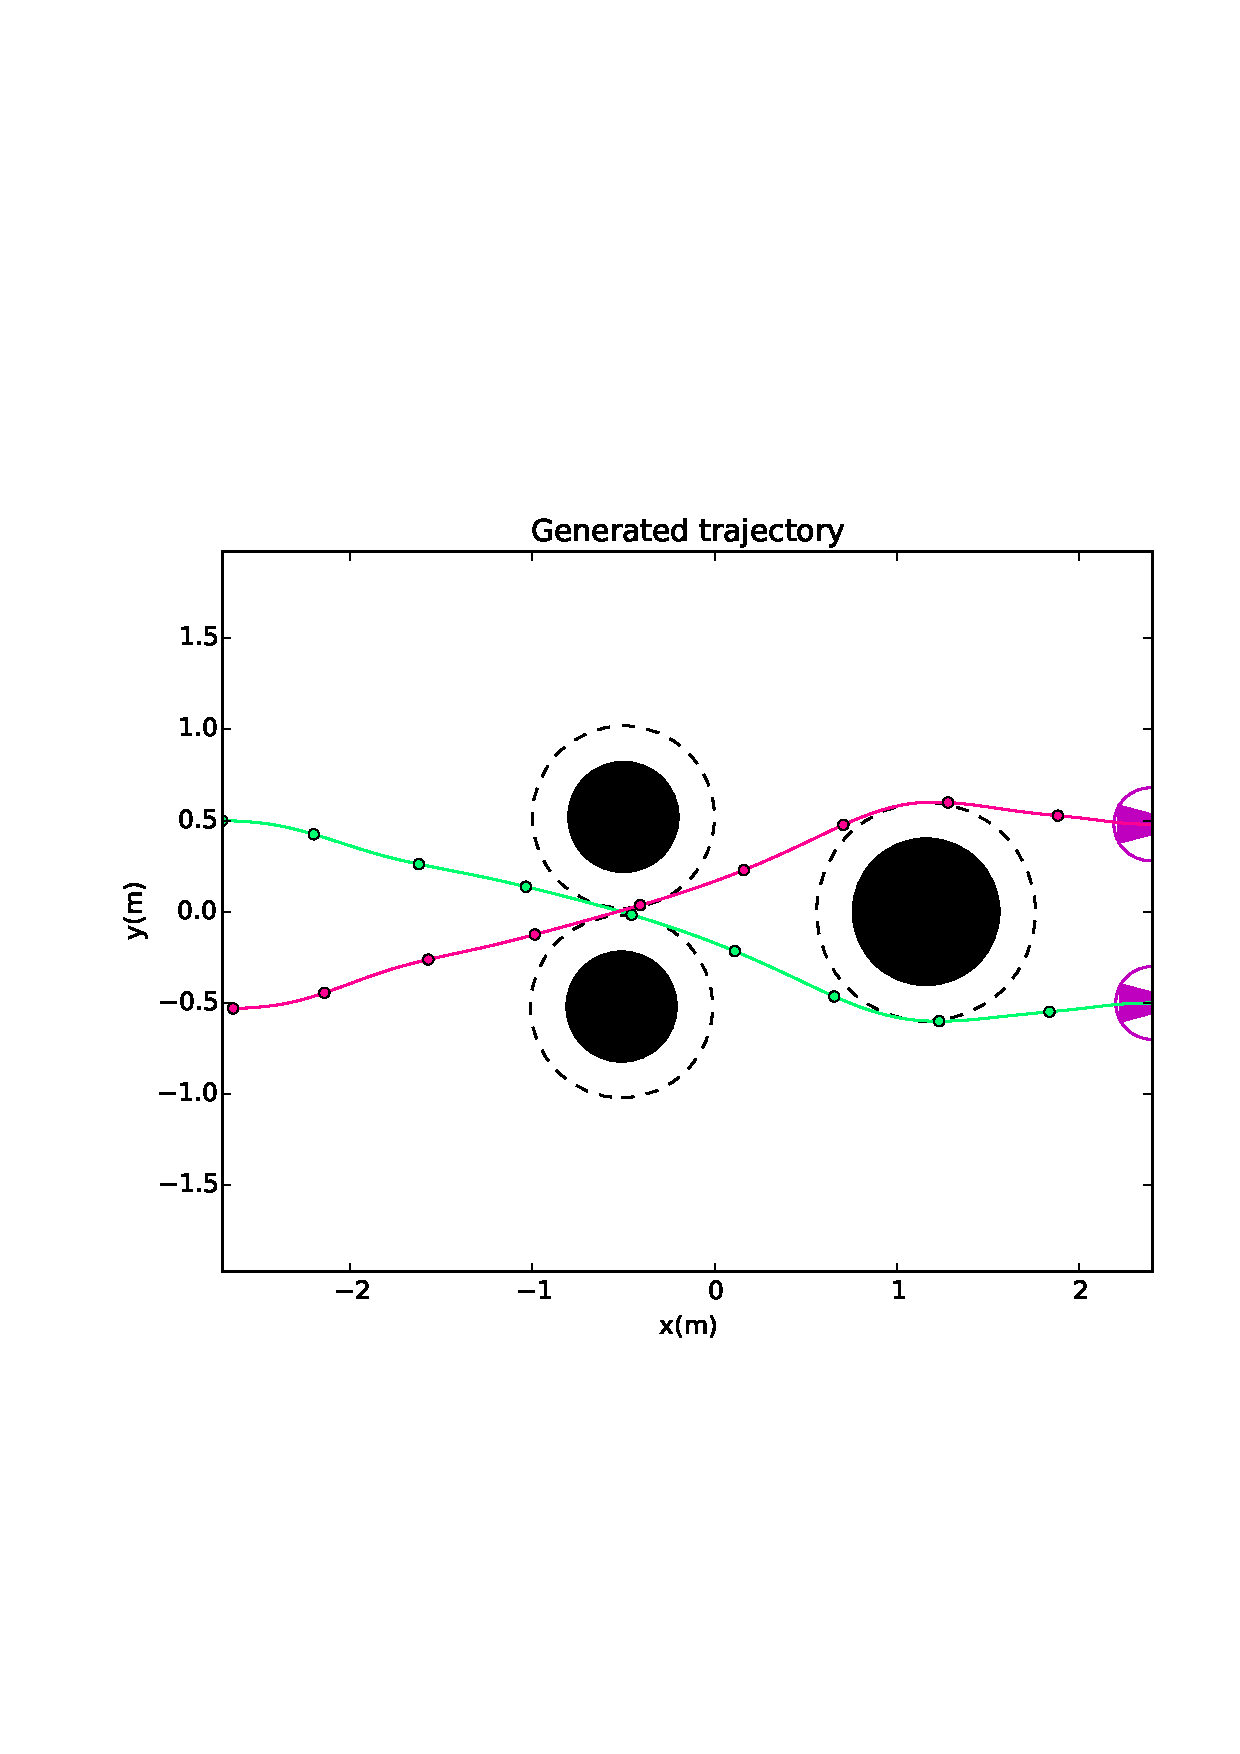
\includegraphics[width=\textwidth]{./images/pwc.png}
                \caption{Generated paths}\label{fig:pwc}
        \end{subfigure}
        ~ %add desired spacing between images, e. g. ~, \quad, \qquad, \hfill etc.
          %(or a blank line to force the subfigure onto a new line)
        \begin{subfigure}[b]{0.48\textwidth}
                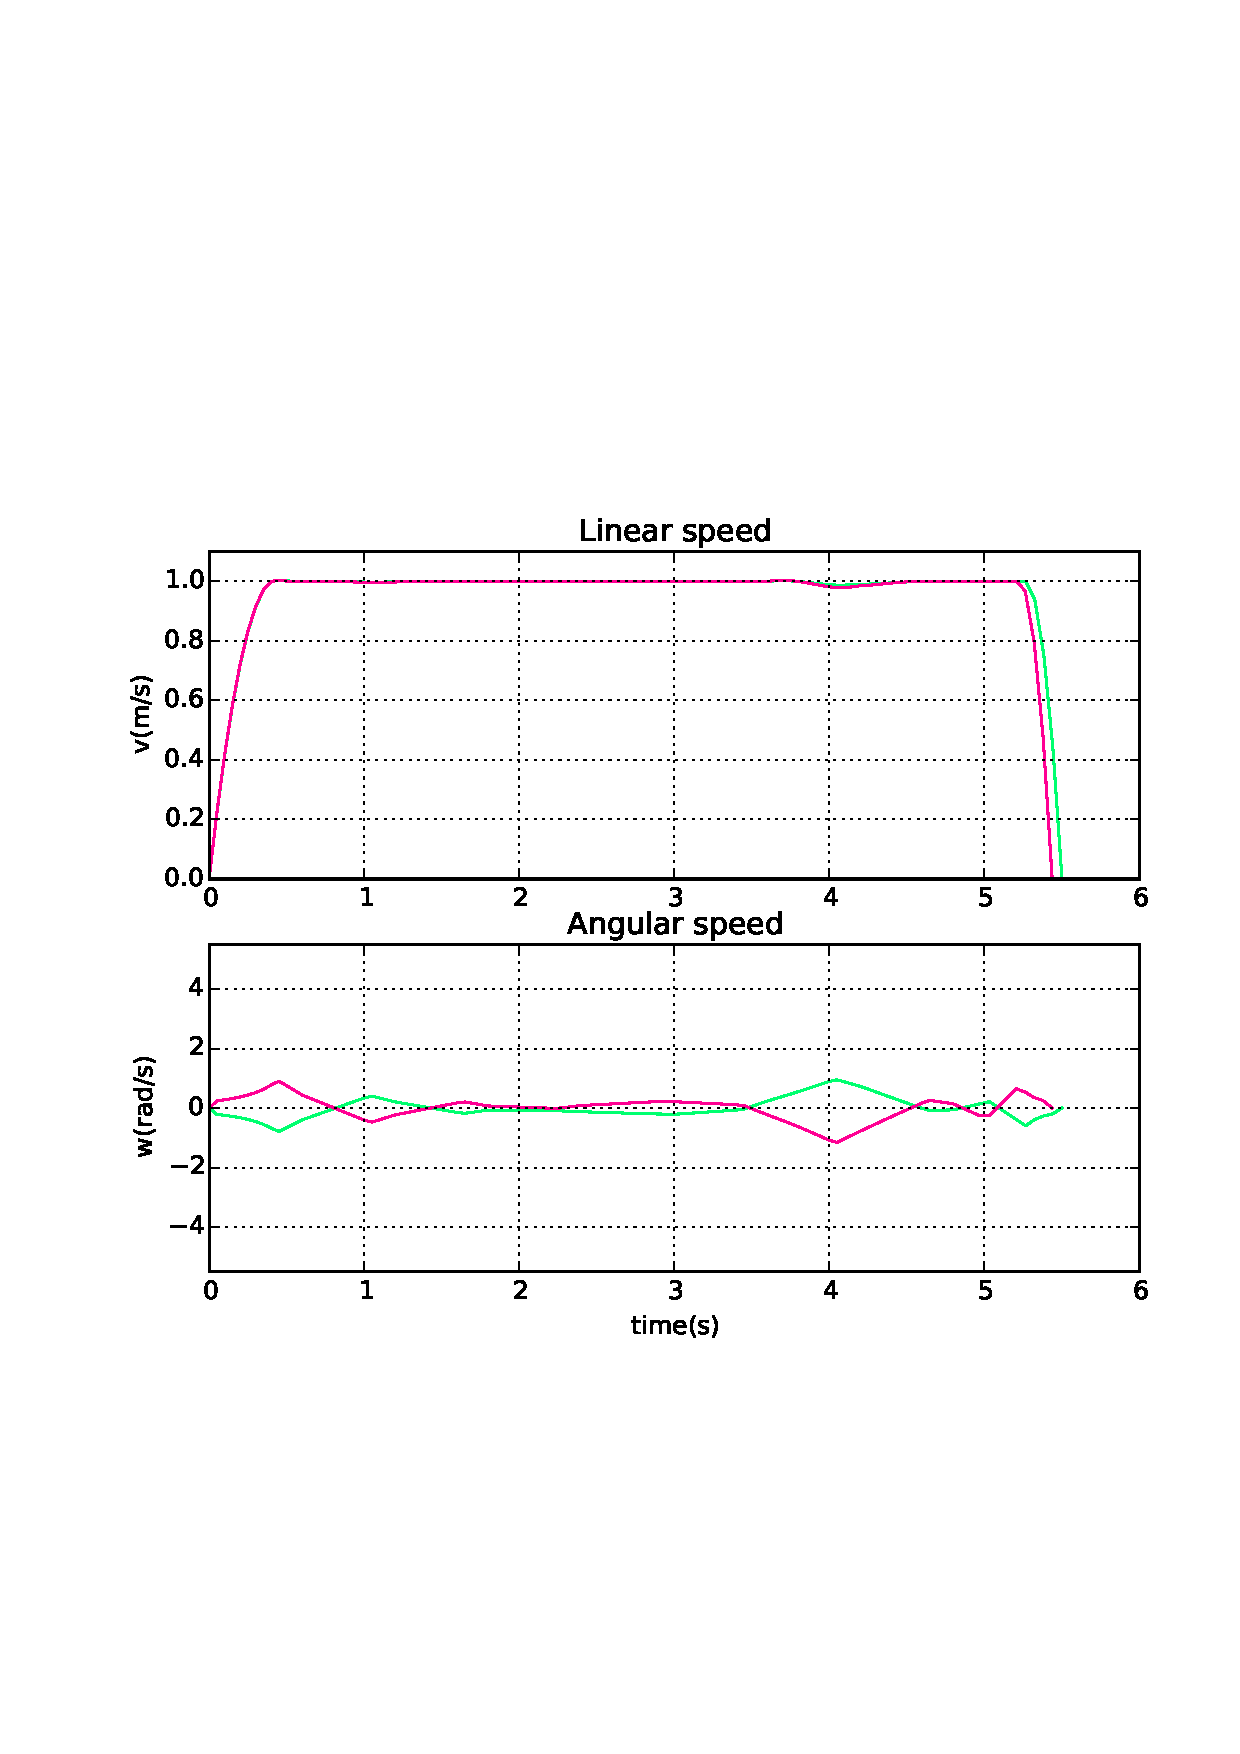
\includegraphics[width=\textwidth]{./images/vwc.png}
                \caption{Velocities}\label{fig:vwc}
        \end{subfigure}
        \caption{Multi-robot path generation without conflict handling.}\label{fig:wc}
\end{figure}

\begin{figure}[!h]
        \centering
        ~ %add desired spacing between images, e. g. ~, \quad, \qquad, \hfill etc.
          %(or a blank line to force the subfigure onto a new line)
        \begin{subfigure}[b]{0.48\textwidth}
                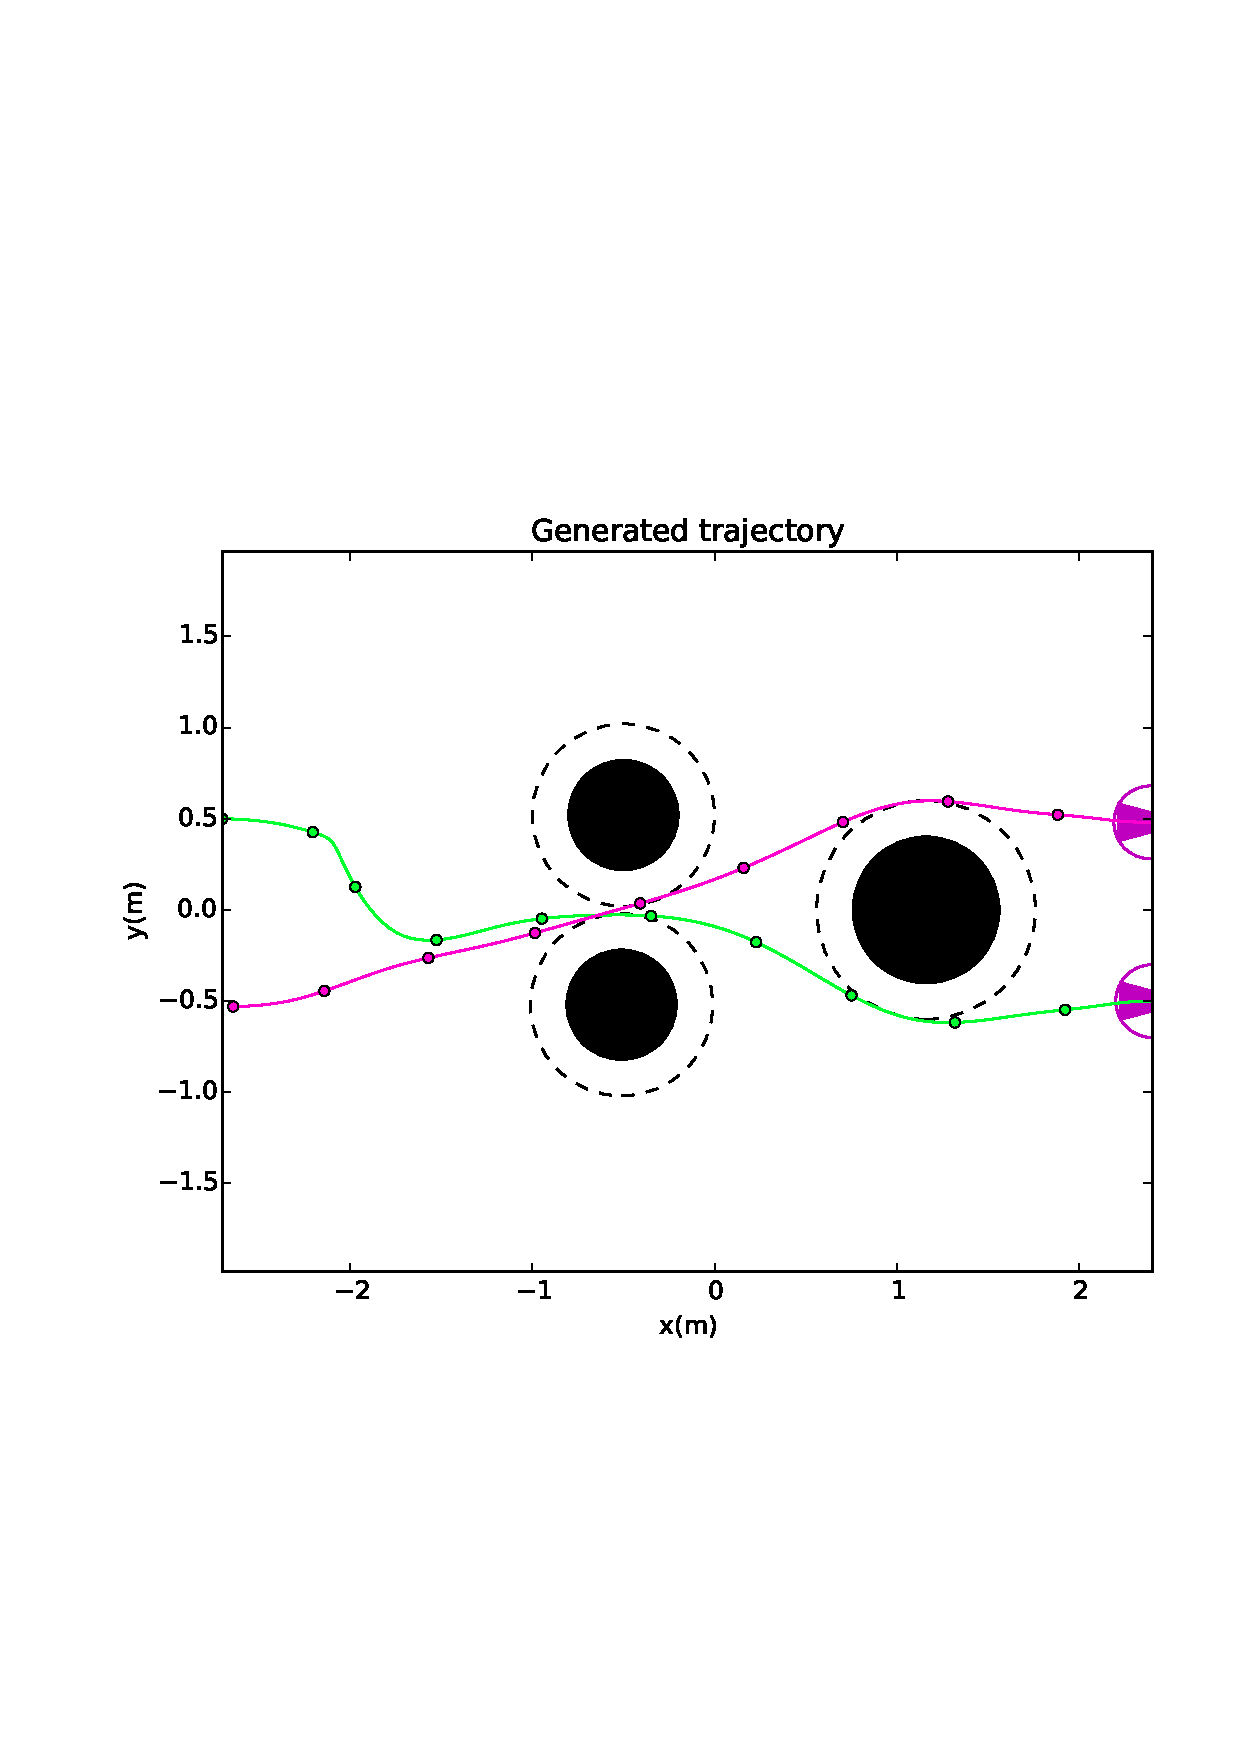
\includegraphics[width=\textwidth]{./images/pnc.png}
                \caption{Generated paths}\label{fig:pnc}
        \end{subfigure}
        ~ %add desired spacing between images, e. g. ~, \quad, \qquad, \hfill etc.
          %(or a blank line to force the subfigure onto a new line)
        \begin{subfigure}[b]{0.48\textwidth}
                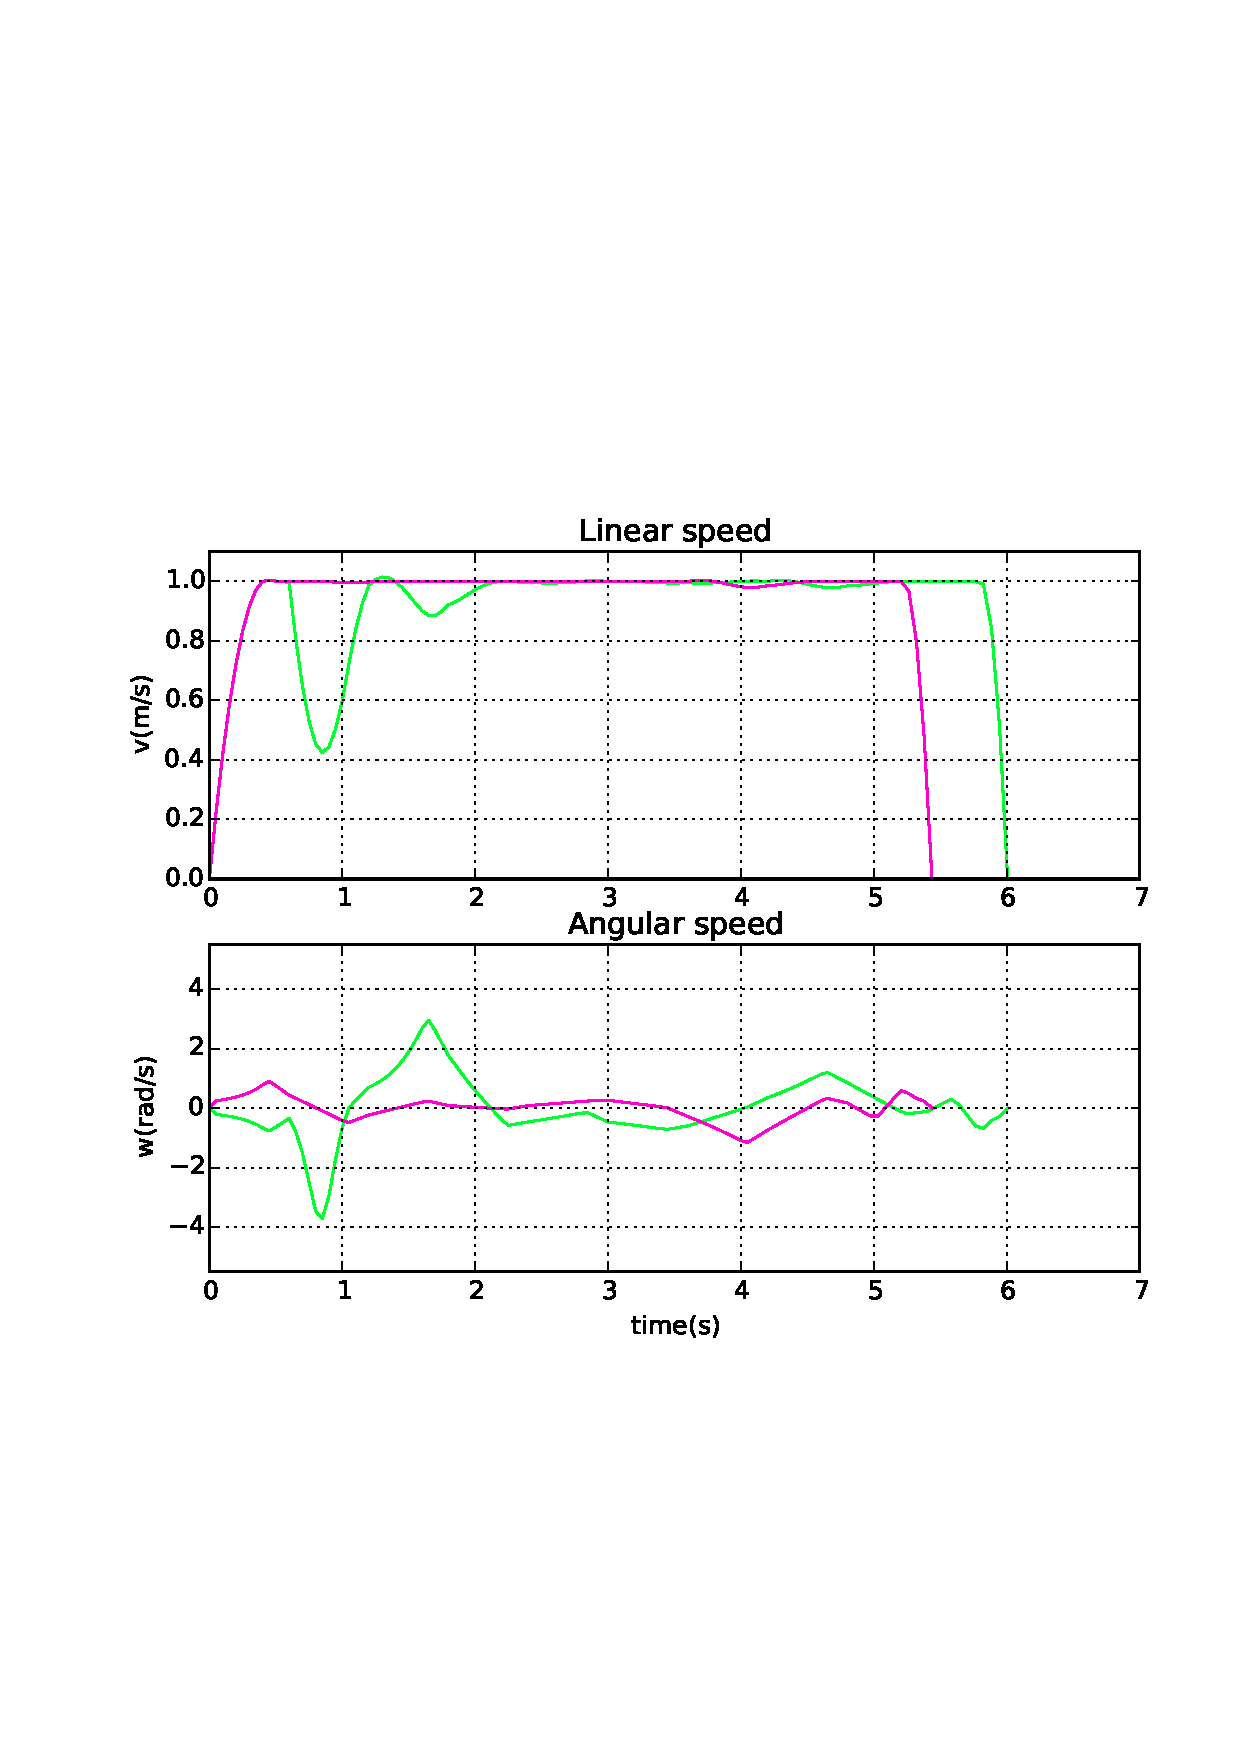
\includegraphics[width=\textwidth]{./images/vnc.png}
                \caption{Velocities}\label{fig:vnc}
        \end{subfigure}
        \caption{Multi-robot path generation with conflict handling.}\label{fig:nc}
\end{figure}

%\clearpage
\subsection{Analyzing the parameters impact on real-time feasibility and solution adequacy}

The performance of the motion planning algorithm previously presented depends on several parameters. For starters these parameters can be split into two groups. The \textbf{algorithm related} parameters and the \textbf{optimization solver related} ones. Among the former group the most important ones are:
\begin{itemize}
\item[$bullet$] The number of sample for time discretization ($N_s$);
\item[$\bullet$] The number of internal knots for the B-splines curves ($n_{knots}$);
\item[$\bullet$] The planning horizon for the sliding window ($T_p$);
\item[$\bullet$] The computation horizon ($T_c$).
\end{itemize}

The latter kind depends on the optimization solver adopted but since most of them are iterative methods it is common to have at least the two following parameters:
\begin{itemize}
\item[$\bullet$] Maximum number of iterations;
\item[$\bullet$] Stop condition.
\end{itemize}

The task of searching for a satisfactory set of parameters' values with regard to a performance metric (e.g. total time to complete the miss1ion) is quite laborious.

We attempted nevertheless to extract some quantitative knowledge about how these parameters impact the generated solution based on several simulations run with different parameters configurations. The main objective here is to be able to support the feasibility of a real-time motion planner based on this algorithm.

Omitting some details about the simulations conditions we present one of the many data used in our analyze in the figures~\ref{fig:uni3} and \ref{fig:r3}. Figure~\ref{fig:r3} shows the solution (path and velocities) for one of the scenarios that were simulated for a given set of parameters listed in the table~\ref{tab:s3param}. Keeping the scenario and varying the parameters we were able to plot the charts on figure \ref{fig:uni3}. We can notice an impact of the number of samples ($N_s$) and number of non-null internal knots ($n_{knots}$) on the \textit{maximum computation time}/$T_c$ ratio. The greater the $n_{knots}$ or the $N_s$ the greater is the \textit{maximum computation time}/$T_c$. This behavior is the one expected since the number of constraints and the number of arguments for the cost function to be minimized depend on these two parameters respectively. Keep in mind that the \textit{maximum computation time}/$T_c$ ratio has to be inferior to one so real-time planning is possible.

We were also able to characterize the influence of the number of obstacles seen at once on the computation time and path quality. As expected the computation time increases with the number of obstacles seen at once.

Finally we proposed some metric to characterize the adequacy of a found solution based on the total time spend going from the initial to the final pose and on the robot to the obstacles distance.

%INFO:R0: TOT: 7.57429378065
%INFO:R0: NSE: 15
%INFO:R0: FIR: 1.07032418251
%INFO:R0: LAS: 0.402824163437
%INFO:R0: LMA: 1
%INFO:R0: MAX: 0.243094921112
%INFO:R0: MIN: 0.0298509597778
%INFO:R0: AVG: 0.156346522845
%INFO:R0: RMP: 0.506447752317
%INFO:R0: RMG: 0.83921700716
%p_3_0.48_2.4_11_4_0.001_15_40_20_5.0_0.1_3.0_0.5_1.0_10.0


\begin{table}[!h]
\caption {Motion planner main parameters} \label{tab:s3param}
\begin{center}
\begin{tabular}{|c|c|}
\hline
$T_p$ & 2.40 s\\
\hline 
$T_c$ & 0.48 s\\
\hline 
$N_s$ & 11\\
\hline 
$n_{knots}$ & 4\\
\hline
$v_{max}$ & $1.00\ \mathrm{m/s}$\\
\hline
$\omega_{max}$ & $5.00\ \mathrm{rad/s}$\\
\hline
$q_{inital}$ & $[-0.05\ 0.00\ \pi/2]^T$\\
\hline
$q_{final}$ & $[0.10\ 7.00\ \pi/2]^T$\\
\hline
$u_{final}$ & $[0.00\ 0.00]^T$\\
\hline
$u_{final}$ & $[0.00\ 0.00]^T$\\
\hline
$O_0$ & $[0.55\ 1.91\ 0.31]$\\
\hline
$O_1$ & $[-0.08\ 3.65\ 0.32]$\\
\hline
$O_2$ & $[0.38\ 4.65\ 0.16]$\\
\hline
\end{tabular}
\end{center}
\end{table}

\begin{figure}[!h]
        \centering
        ~ %add desired spacing between images, e. g. ~, \quad, \qquad, \hfill etc.
          %(or a blank line to force the subfigure onto a new line)
        \begin{subfigure}[b]{0.48\textwidth}
                \includegraphics[width=\textwidth]{./images/realtime/sim_results/p_3_0.48_2.4_11_4_0.001_15_40_20_5.0_0.1_3.0_0.5_1.0_10.0/multirobot-path.png}
                \caption{Robot's path.}\label{fig:rpath}
        \end{subfigure}
        ~ %add desired spacing between images, e. g. ~, \quad, \qquad, \hfill etc.
          %(or a blank line to force the subfigure onto a new line)
        \begin{subfigure}[b]{0.48\textwidth}
		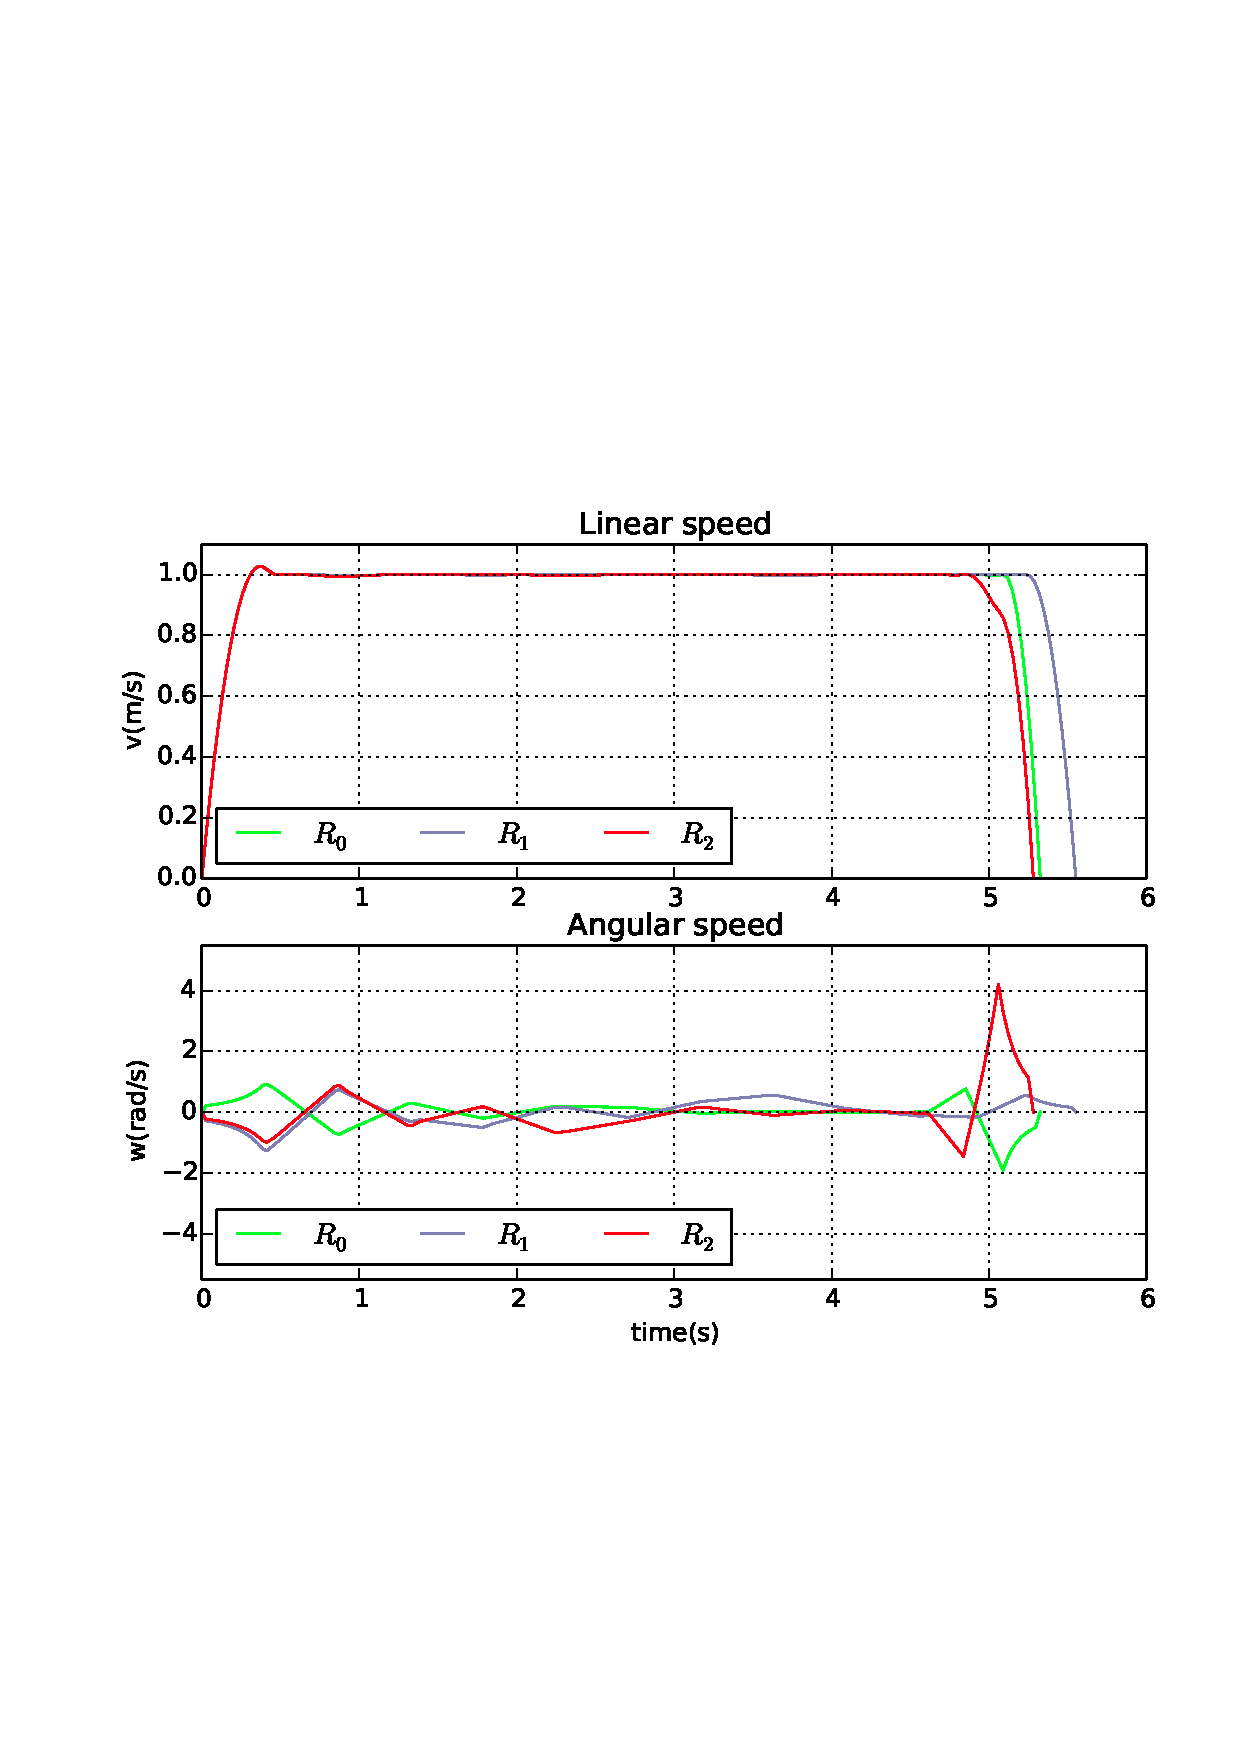
\includegraphics[width=\textwidth]{./images/realtime/sim_results/p_3_0.48_2.4_11_4_0.001_15_40_20_5.0_0.1_3.0_0.5_1.0_10.0/multirobot-vw.png}
                \caption{Robot's input.}\label{fig:rinput}
        \end{subfigure}
        \caption{Three obstacles scenario simulation example where the \textit{maximum computation time} was about 84\% of $T_c$ and the mission total time equals to $7.57\ s$.}\label{fig:r3}
\end{figure}

\begin{figure}[!h]
        \centering
        ~ %add desired spacing between images, e. g. ~, \quad, \qquad, \hfill etc.
          %(or a blank line to force the subfigure onto a new line)
        \begin{subfigure}[b]{0.48\textwidth}
                \includegraphics[width=\textwidth]{./images/realtime/Scenario_3__N_knots_4/mcttc-tctp.eps}
                \caption{Four internal knots. Average variance between lines is $1.047\times 10^{-2}$}\label{fig:uni34}
        \end{subfigure}
        
        ~ %add desired spacing between images, e. g. ~, \quad, \qquad, \hfill etc.
          %(or a blank line to force the subfigure onto a new line)
        \begin{subfigure}[b]{0.48\textwidth}
                \includegraphics[width=\textwidth]{./images/realtime/Scenario_3__N_knots_5/mcttc-tctp.eps}
                \caption{Five internal knots. Average variance between lines is $0.972\times 10^{-2}$}\label{fig:uni35}
        \end{subfigure}
        ~ %add desired spacing between images, e. g. ~, \quad, \qquad, \hfill etc.
          %(or a blank line to force the subfigure onto a new line)
        \begin{subfigure}[b]{0.48\textwidth}
                \includegraphics[width=\textwidth]{./images/realtime/Scenario_3__N_knots_6/mcttc-tctp.eps}
                \caption{Six internal knots. Average variance between lines is $0.587\times 10^{-2}$}\label{fig:uni36}
        \end{subfigure}
        \caption{Three obstacles scenario.}\label{fig:uni3}
\end{figure}


%\clearpage
\subsection{From Python to XDE simulator}

XDE is a physics simulation software environment fully developed by CEA-LIST that can handle a variety of physical aspects such as deformable bodies, multibody systems with kinematic constraints and contacts, and fluids.

Its utilization presents though some rough edges and a steep learning curve.

During the third month and beginning of the forth while producing the analysis referenced by the latest subsection we begin porting the implementation done in python to the XDE environment. 

The objective is to get much closer to a real physical system being able to implement dynamic behavior in the simulated environment which was previously neglected.
%For instance the obstacle detection can be based on real sensors models carrying uncertainties instead of assuming the absolute knowledge of an obstacle position as soon as it enters within the robot's detection radius.

% \todo[inline, color=green!40]{develop this article}
% \cite{Gao2006}
%\clearpage
\section{Discussions}
% \todo[inline, color=green!40]{Quels sont les avantages et inconvénients des techniques étudiées ? Quelles sont les limites de ces méthodes ? Quelles sont les hypothèses "cachées" que font ces méthodes ? ...}

We implemented and did some minors improvements on the solution proposed by \cite{Defoort2007a} and we gather a good understanding of the impact of the algorithm's parameters in the computation cost and in the quality of the solution.

% qualities
The implemented algorithm has the quality of dealing with multi-robot systems in a robust manner, handling collision as well as lost of communication conflicts without greatly increasing the computation time.

Besides, thanks to the reduction of the solution's search space by creating a parametric representation of the trajectory, this algorithm can respect real-time constraints for a multi-robot system evolving in a unknown environment where static obstacles are present.

The biggest drawback of this approach is how to choose a set of parameters (algorithm and numerical solver related) well adapted to a given scenario. We were able to identify the parameters that has a bigger influence on the solution adequacy and computation time. The number of samples ($N_s$) is the parameter that greatly impacts the computing time followed by the number of obstacles detected at once by the robot (defined by the detection radius and the obstacles positioning with respect to the robot). In the other hand, the solution adequacy depends highly on the $N_s/T_p$ ratio and on the number of internal knots of the B-spline representation $n_{knots}$.


%\clearpage
\section{Perspectives}
% \todo[inline, color=green!40]{Est-ce que le problème est résolu ? Quels axes d'amélioration peut-on envisager ?}

During the months to come we hope to finish the implementation of the C++ code in the XDE simulator and develop the current approach so it can address dynamic obstacles.

We plan to write a paper focusing on the impact of the algorithm's parameters on the computation cost and on the solution quality  for submitting to the International Workshop on On-line Decision-Making in Multi-Robot Coordination.


% Commands to include a figure:
% \begin{figure}
% \centering
% \includegraphics[width=0.5\textwidth]{frog.jpg}
% \caption{\label{fig:frog}This is a figure caption.}
% \end{figure}


% \bibliographystyle{unsrt}
%\clearpage
\selectlanguage{english}
%\nocite{*}
\bibliography{references}
\bibliographystyle{plain}


\end{document} to your LaTeX file where you want your
% title page.
%
%%%%%%%%%%%%%%%%%%%%%%%%%%%%%%%%%%%%%%%%%
%----------------------------------------------------------------------------------------
%	PACKAGES AND OTHER DOCUMENT CONFIGURATIONS
%----------------------------------------------------------------------------------------

\documentclass[12pt]{article}

\usepackage[T1]{fontenc}
\usepackage[utf8]{inputenc}
\usepackage[a4paper, left=2.8cm, right=2.0cm, top=3.0cm, bottom=3.0cm]{geometry}
\usepackage{graphicx}
\usepackage{amsmath, amssymb, amsfonts, amsthm}
\usepackage{float}
\usepackage{color}
\usepackage[english, french]{babel}
\usepackage{lipsum}
\usepackage{float}
%\usepackage{makeidx}
\usepackage{setspace}
\usepackage{url}
\usepackage[table]{xcolor}
\usepackage[nottoc]{tocbibind}
\usepackage{parcolumns}
\usepackage{fancyhdr}
\usepackage{tikz}
\usepackage{caption}
\usepackage{subcaption}
% \usepackage[enable]{easy-todo}
\usepackage{xargs}
\usepackage[colorinlistoftodos,prependcaption,textsize=tiny]{todonotes}
\usepackage{soul}
\usepackage{epstopdf}

\newcommandx{\change}[2][1=]{\todo[linecolor=red,backgroundcolor=red!25,bordercolor=red,#1]{#2}}

\newtheorem{problem}{Problem}
\newtheorem{theorem}{Theorem}
\newtheorem{lemma}{Lemma}
\newtheorem{example}{Example}
\newtheorem{remark}{Remark}
\newtheorem{definition}{Definition}
\newtheorem{proposition}{Proposition}
\newtheorem{corollary}{Corollorary}
\newtheorem{conjecture}{Conjecture}
\newtheorem{idea}{Idea}

\title{PFE-WrittenReport}
\author{MENDES FILHO, José Magno}

\newcommand{\N}{\mathbb{N}}
\newcommand{\R}{\mathbb{R}}
\newcommand{\Z}{\mathbb{Z}}

\numberwithin{equation}{section}

\newenvironment{abstractpage}
  {\cleardoublepage\vspace*{\fill}\thispagestyle{empty}}
  {\vfill\cleardoublepage}
\newenvironment{Abstract}[1]
  {\bigskip\selectlanguage{#1}%
   \begin{center}\bfseries\abstractname\end{center}}
  {\par\bigskip}

\begin{document}

%=======%
% TITLE %
%=======%

\begin{titlepage}

\newcommand{\HRule}{\rule{\linewidth}{0.5mm}}
\center

% Logos
\begin{minipage}{0.32\textwidth}
%\begin{center}
\begin{flushleft}
	\includegraphics[height=4.0cm]{./images/logo_ensta.jpg}
\end{flushleft}
\end{minipage}
\begin{minipage}{0.32\textwidth}
\begin{center}
	\includegraphics[height=1.6cm]{./images/upmc.png}
\end{center}
\end{minipage}
\begin{minipage}{0.32\textwidth}
\begin{flushright}
	\includegraphics[height=2.7cm]{./images/cea.png}
\end{flushright}
\end{minipage}
\mbox{}\\[1.5cm]

\selectlanguage{french}

\textsc{\LARGE PFE - rapport mi-parcours}\\[0.3cm]
\textsc{\Large Robotique et Systèmes Embarqués}\\[0.3cm]
\Large{2014/2015}\\[0.6cm]

\selectlanguage{english}

{Réf : DIASI / 15-351 \hfill}

\HRule \\[0.2cm]
\Huge \textbf{Local Dynamic Path Planning for an Autonomous Forklift in Human Environment}\\[-0.2cm] % Title
\HRule \\[0.5cm]

\begin{center}
\textbf{\textcolor{red}{\Large{
Unclassified Report}\\[-0.4cm]% Classified
\large{Can be made public on the internet}
}}
\end{center}

\begin{minipage}{0.55\textwidth}
\begin{flushleft} \Large
\emph{Author:}\\
José Magno \textsc{Mendes Filho} \\[0.7cm] % Author
\end{flushleft}
\end{minipage}
~
\begin{minipage}{0.35\textwidth}
\begin{flushright} \Large
\mbox{}\\[0.4cm]
Promotion 2014
\end{flushright}
\end{minipage}\\[1.0cm]

\begin{minipage}{0.45\textwidth}
\begin{flushleft} \large
\emph{Supervisor - ENSTA:}\\
David \textsc{Filliat} % Tuteur ENSTA
\end{flushleft}
\end{minipage}
~
\begin{minipage}{0.45\textwidth}
\begin{flushright} \large
\emph{Supervisor - CEA:} \\
Éric \textsc{Lucet} % Tuteur Ailleurs
\end{flushright}
\end{minipage}\\[1.0cm]

\large{Internship from 05 Mars 2015 to 28 August 2015}\\[0.6cm]
\large{CEA LIST Digiteo Moulon\\ Bât. 660 91191 GIF-SUR-YVETTE Cedex, France}
\end{titlepage}
%\thispagestyle{empty}

%\onehalfspace
%\frontmatter
%\cleardoublepage

\pagestyle{fancy}
\fancyhead{}
%\fancyhead[LE,RO]{\rightmark} %section
\fancyhead[RE,LO]{\leftmark} %chapter
\fancyfoot{}
\cfoot{\textsc{Mendes Filho} José Magno - CEA\\\textcolor{red}{Unclassified - Can be made public on the internet}}
\fancyfoot[OR,EL]{\thepage}

% Pour cette synthèse, vous devez choisir un sujet et faire une courte bibliographie en choisissant au moins 3 articles scientifiques. Vous devez m'envoyer un rapport de 3 pages max synthétisant ces articles selon le plan suivant:
% - Introduction : quel est le problème ? dans quel contexte le trouve t'on ? quel est  l'utilité de savoir le résoudre ? ...
% - Etat de l'art : présentation rapide des techniques des articles étudiés, de leur points communs et de leur différences....
% - Discussion : Quels sont les avantages et inconvénients des techniques étudiées ? Quelles sont les limites de ces méthodes ? Quelles sont les hypothèses "cachées" que font ces méthodes ? ...
% - Perspectives : Est-ce que le problème est résolu ? Quels axes d'amélioration peut-on envisager ?

% \begin{abstract}
% Your abstract.
% \end{abstract}
\selectlanguage{english}
\section{Introduction}

% \todo[inline, color=green!40]{quel est le problème ? dans quel contexte le trouve t'on ? quel est  l'utilité de savoir le résoudre ?}

This document is meant to describe the work done until now as well as the partial results and the perspectives for my final year internship as an engineering student at ENSTA ParisTech and UPMC - Paris VI.

The first two months of this internship toke place at the "Unité Informatique et Ingénierie des Systèmes" at ENSTA under the supervision of David Filliat. After that, from May to the present I have been working at CEA LIST Digiteo Moulon under the supervision of Eric Lucet.

\subsection{Internship context}

The work developed during this internship falls within the context of an applied research project on automation of a forklift truck for the effective supply of assembly lines.

Thus, the mobile robot has to be able to evolve in a partially known, shared with humans environment while being efficient with respect to time and energy spend on its tasks and preserving the workers' safety.

\subsection{Objectives}

The main objective of this internship is to implement, test, evaluate and improve an experimental path planning algorithm presented in details in~\cite{Defoort2007a} with respect to its applicability to a scenario where autonomous forklift trucks and humans share the same environment. This experimental planning algorithm consists in planning the mobile robot's path by solving a direct trajectory optimization problem~\cite{betts1998survey} using B-splines for representing the system flat output~\cite{milam2003real}. 

As stated~\cite{Defoort2007a} this approach presents good advantages for multi-robots systems evolving in an uncertain environment with static obstacles over other solutions. For instance, analytic methods are inapplicable for nonholonomic systems in presence of obstacles. Cell decomposition methods have the downside of requiring a \textit{a priori} space modeling. The dynamic window approach does not seem flexible enough to be extended to a multi-robot system.

The two main challenges that may be confronted during this work is how to guarantee real-time property for our specific application and how to generalize the algorithm in order to account for humans, i.e. dynamic obstacles.

\clearpage
\section{Initial achievements}
\label{sec:etatdelart}

% \todo[inline, color=green!40]{présentation rapide des techniques des articles étudiés, de leur points communs et de leur différences....}

During the first two months of this work we focused in understanding and reproducing the trajectory generation algorithm presented in~\cite{Defoort2007a} going from a single robot global planning method to a multi-robot local real-time planning. During the third month we focused in the analysis of the impact of different parameters in the method performance and feasibility.

\subsection{Nonlinear programming problem (NLP)}

Firstly we studied how the path planning problem could be translated into a nonlinear programming problem by intelligently using the mobile robot's model flatness property and representing the trajectory by B-splines.

\subsubsection{Problem Formulation}

Let us briefly and without mathematical rigor present how the problem of finding a collision-free, optimized path for a mobile robot represented by a unicycle model can be written.

The equation~\ref{eq:unic} represents the unicycle kinematic model. Thanks to the flatness property it is possible to be only interested in planning a trajectory for the flat output variable $z$ where $z = [x,\ y]^T$.

\begin{equation}\label{eq:unic}
\begin{array}{c}
\dot{q} = \mathrm{f}(q, u) \Rightarrow\\
\left[\begin{array}{c}
\dot{x}\\
\dot{y}\\
\dot{\theta}
\end{array}\right]=
\left[\begin{array}{c}
v\cos(\theta)\\
v\sin(\theta)\\
w
\end{array}\right]
\end{array}    
\end{equation}

The equations \ref{eq:phi1}, \ref{eq:phi2} show how the state variables and control variables can be calculated from the flat output and its first $l^{th}$ derivatives. This way, whenever we need to retrieve the fundamental variables we can by means of these equations.

\begin{equation}\label{eq:phi1}
            \begin{array}{l}
            \varphi_1(z(t_k),\dotsc,z^{(l)}(t_k))=\\
            \left[\begin{array}{c}
            x\\
            y\\
            \theta
            \end{array}\right]
            \left[\begin{array}{c}
            z_1\\
            z_2\\
            \arctan(\dot{z}_2/\dot{z}_1)\\
            \end{array}\right]
            \end{array}
\end{equation}

\begin{equation}\label{eq:phi2}
\begin{array}{l}
            \varphi_2(z(t_k),\dotsc,z^{(l)}(t_k))=\\
            \left[\begin{array}{c}
            v\\
            \omega
            \end{array}\right]
            = \left[\begin{array}{c}
            \sqrt{\dot{z}_{1}^{2} + \dot{z}_{2}^{2}}\\
            \dfrac{\dot{z}_{1}\ddot{z}_{2} -
            \dot{z}_{2}\ddot{z}_{1}}{\dot{z}_{1}^{2}+\dot{z}_{2}^{2}}
            \end{array}\right]
            \end{array}
\end{equation}

%\begin{equation}\label{eq:phi3}
%\begin{array}{l}
%            \varphi_3(z(t_k),\dotsc,z^{(l)}(t_k))=\\
%            \left[\begin{array}{c}
%            \dot{v}\\
%            \dot{\omega}
%            \end{array}\right]
%            = \left[\begin{array}{c}
%            \frac{\partial}{\partial t}v\\
%            \frac{\partial}{\partial t}\omega
%            \end{array}\right]
%            = \left[\begin{array}{c}
%            \frac{\dot{z}_1\ddot{z}_1 + \dot{z}_2\ddot{z}_2}{\|\dot{z}\|}\\
%            \frac{(\ddot{z}_1\ddot{z}_2+ z^{(3)}_2\dot{z}_1 - (\ddot{z}_2\ddot{z}_1+z^{(3)}_1\dot{z}_2))\|\dot{z}\|^2- 2(\dot{z}_1\ddot{z}_2-\dot{z}_2\ddot{z}_1)\|\dot{z}\|\dot{v}}{\|\dot{z}\|^4}
%            \end{array}\right]
%            \end{array}
%\end{equation}

Now let us write the NPL problem that minimizes the square of the time spend (\ref{eq:objective}) to go from a $q_{initial}$ pose at a $u_{initial}$ velocity to a $q_{final}$ pose at a $u_{final}$ velocity, avoiding $M$ static obstacles represented by circles with radius $r_m$\footnote{the own robot geometry is here represented by a circle of radius $\rho$}, having velocities in an admissible velocity set denoted by $\mathcal{U}$.

\begin{equation}\label{eq:objective}
	\underset{(t_{final},C_0,\dotsc,C_{d+n_{knot}-2})}{\mathrm{min}} J = (t_{final}-t_{initial})^{2}
\end{equation}

under the following constraints $\forall k \in \{0,\dotsc,N_s -1\}$ and $\forall m \in {0,\dotsc,M-1}$:
\begin{equation}%\label{eq:sysr4}
\left\lbrace\begin{array}{lcl}
    \varphi_1(z(t_{initial}),\dotsc,z^{(l-1)}(t_{initial})) & = & q_{initial}\\
    \varphi_1(z(t_{final}),\dotsc,z^{(l-1)}(t_{final})) & = & q_{final}\\
    \varphi_2(z(t_{initial}),\dotsc,z^{(l)}(t_{initial})) & = & u_{initial}\\
    \varphi_2(z(t_{final}),\dotsc,z^{(l)}(t_{final}))& = & u_{final}\\
    \varphi_2(z(t_k),\dotsc,z^{(l)}(t_k)) &\in& \mathcal{U}\\
    d_{O_m}(t_k) &\geq& \rho + r_m,\quad \forall O_m \in \mathcal{Q}_{occupied}
\end{array}\right.
\end{equation}

\subsubsection{Implementation of the solution}

Once we were able to write the problem as above the subsequent step was to implement this planning method using some programming language. We kept in mind that a high level language provided with some NLP solver package would be preferable.

We decided to use Python language and the Scipy package. Within the Scipy module many minimization methods can be found. For this specific optimization problem, only the method SLSPQ was appropriate. It was the only one to handle constrained minimization where the constraints could be equations as well as inequations.

Since the SLSPQ is a local optimization method the first guess used for initializing the solver had an impact on the time of convergence as well as on the found solution. A bad first guess can prevent the solver for converging at all, as shown in the figure~\ref{fig:planning-sim-trajc}.

Besides the bad first guess we notice another problem that could cause the Scipy implementation of the SLSQP solver to not converge. A too big cost value for the objective function (for instance, for values greater then $10^6$) could also prevent the convergence of the solver.

\begin{figure}[!h]
	\centering
	\includegraphics[width=0.6\textwidth]{./images/planning-sim-trajc.png}
	\caption{Path resulting from a bad initialisation.\label{fig:planning-sim-trajc}}
\end{figure}

An initialization algorithm was then proposed along some changes in the objective function evaluation so better solutions could be achieved quicker.

The initialization algorithm is a simple one that interactively changes the positions of the B-splines control points in order to prevent the initial trajectory guess to pass between two obstacles that are too close together (distance inter-obstacle smaller than the robot diameter).

\subsection{Evolving from the previous NLP to the sliding window multi-robot decentralized approach}

Solving the problem as stated in the previous subsection is only worth considering as a base initial solution to our problem.
%We are interested here in a real-time local planner that evolves in a %partially known environment suited for a multi-robot fleet.

Following the work done in~\cite{Defoort2007a} we built over the first implementation so to have a strongly decentralized planner for multi-robot fleet that is collision-free with respect to the robots in the fleet as well as to static obstacles as before. This new approach was suitable for real-time implementation as well. We chose a strongly decentralized approach over a centralized one so no central supervisor is needed and so we can keep the computation complexity of solving the trajectory optimization problem close to the one in a single robot system.

Using a sliding window in time the new planner produced a "per robot" intended trajectory meant to be valid within a planning horizon that was locally optimal with respect to a new objective function and collision-free only with respected to the static obstacles.

The presence of other robots is taken into account in a second moment: the intended trajectory is updated after the robots involved in a possible future conflict exchange their intended trajectories so no conflict (collision or lost of communication) occur for the corrected new trajectory.

Figures \ref{fig:wc} and \ref{fig:nc} show two multi-robot local planning without and with collision handling.

\begin{figure}[!h]
        \centering
        ~ %add desired spacing between images, e. g. ~, \quad, \qquad, \hfill etc.
          %(or a blank line to force the subfigure onto a new line)
        \begin{subfigure}[b]{0.48\textwidth}
                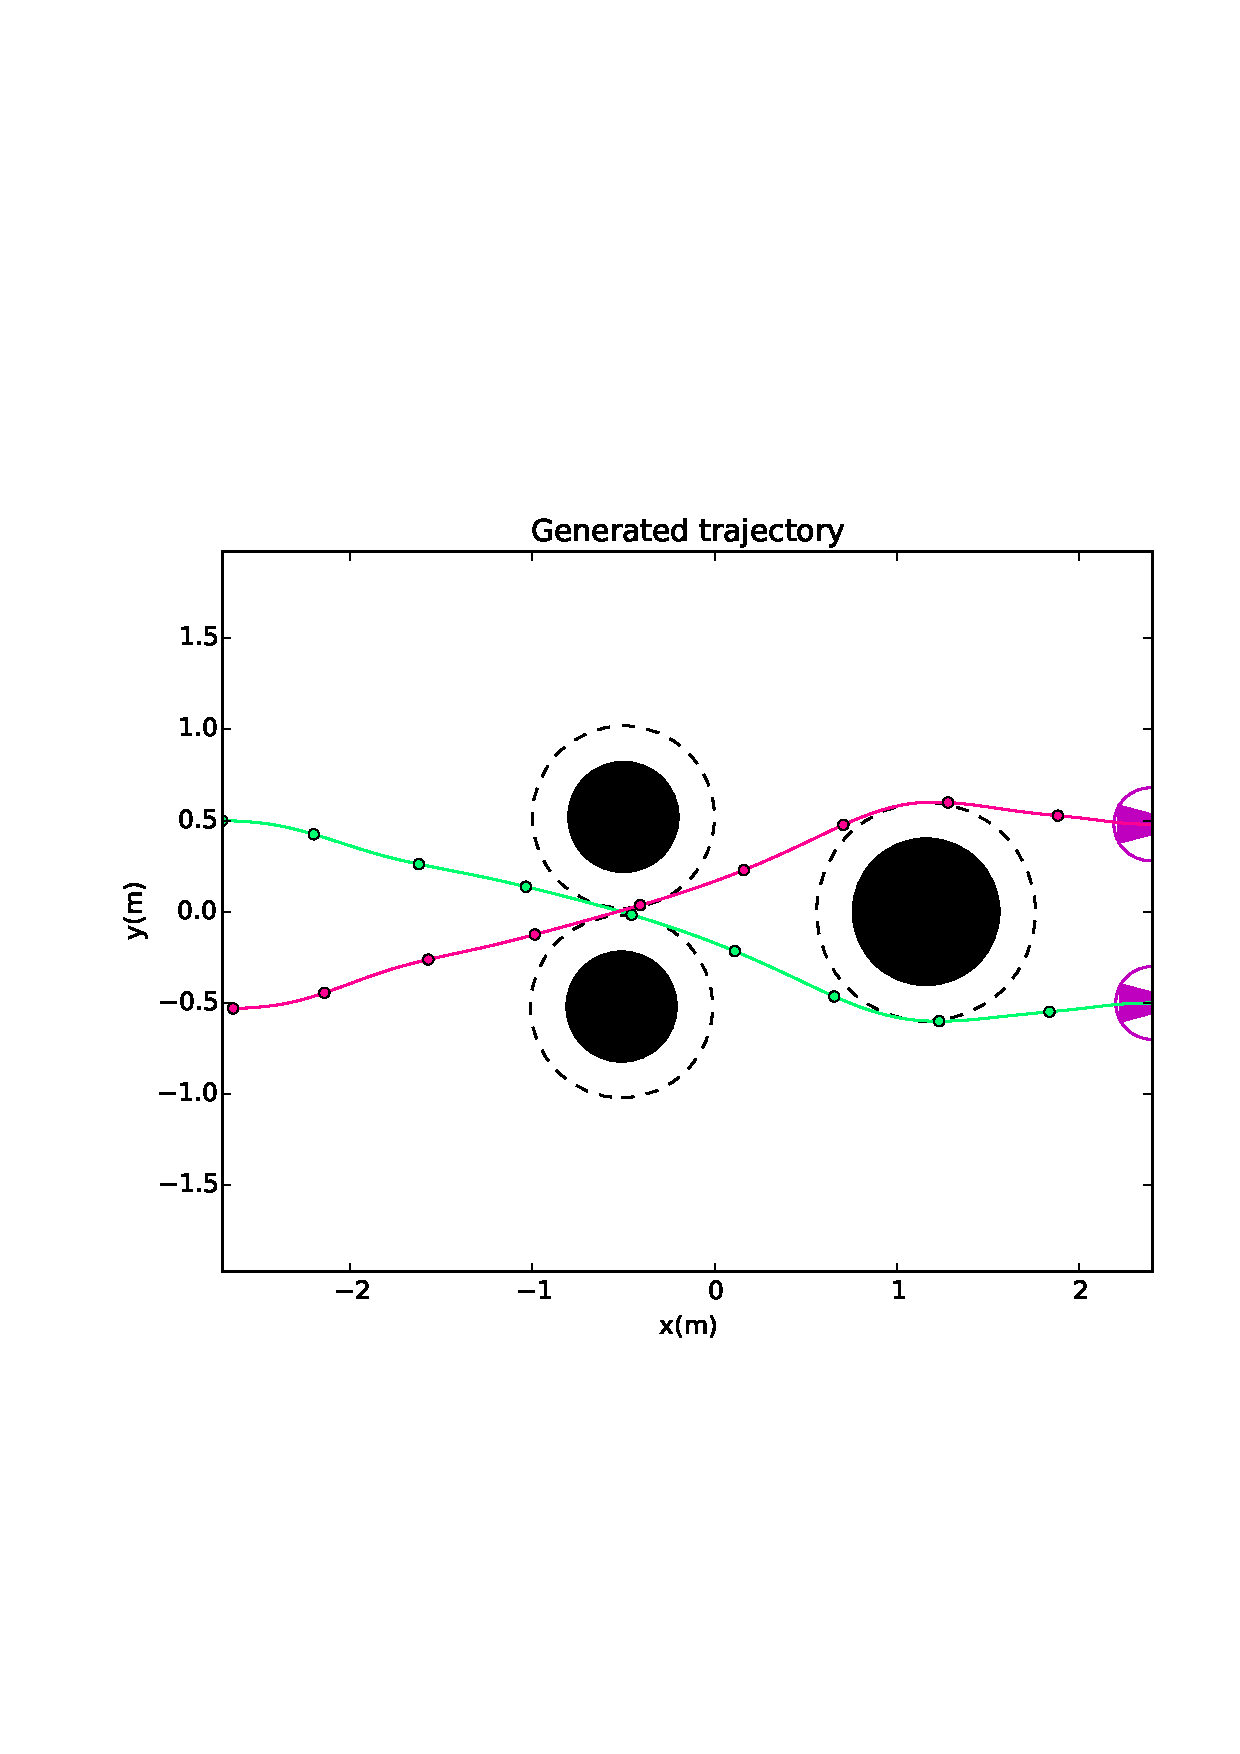
\includegraphics[width=\textwidth]{./images/pwc.png}
                \caption{Generated paths}\label{fig:pwc}
        \end{subfigure}
        ~ %add desired spacing between images, e. g. ~, \quad, \qquad, \hfill etc.
          %(or a blank line to force the subfigure onto a new line)
        \begin{subfigure}[b]{0.48\textwidth}
                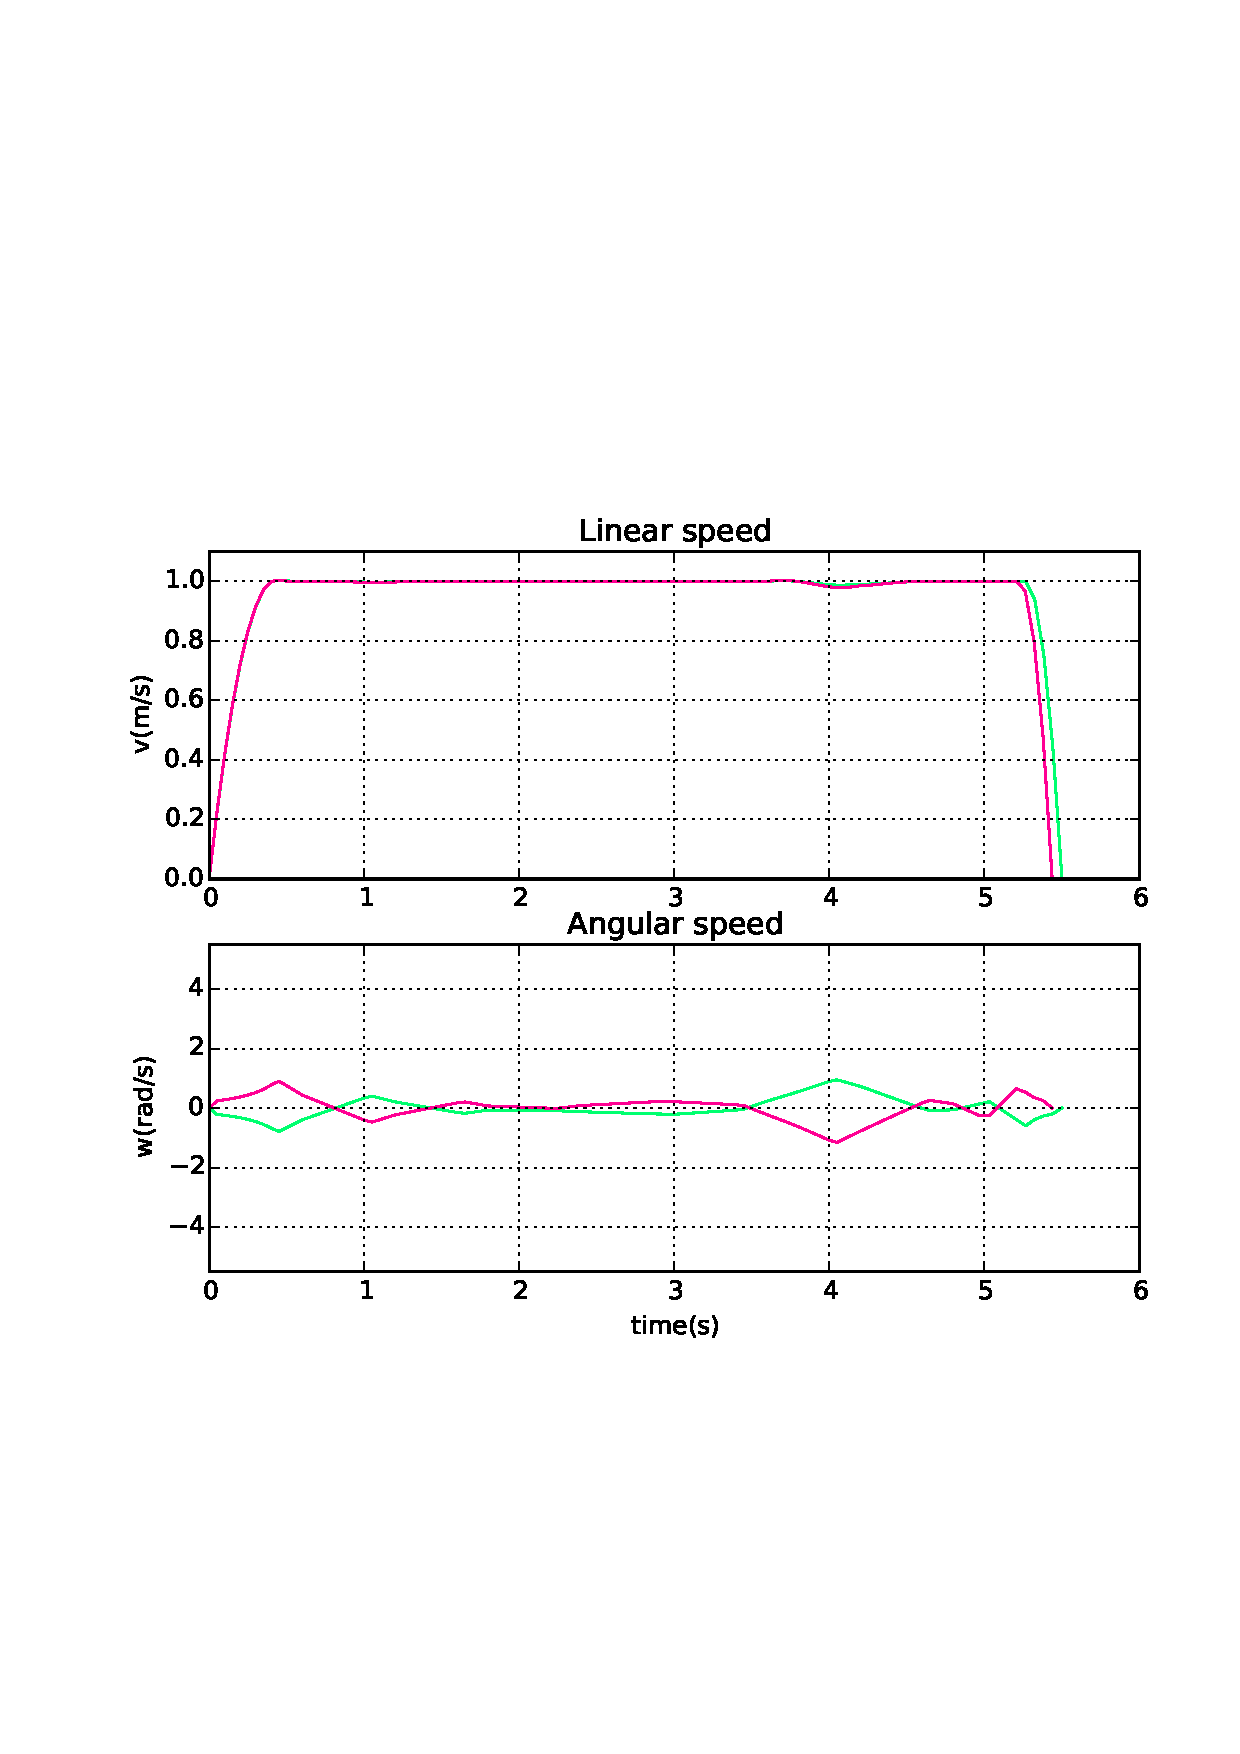
\includegraphics[width=\textwidth]{./images/vwc.png}
                \caption{Velocities}\label{fig:vwc}
        \end{subfigure}
        \caption{Multi-robot path generation without conflict handling.}\label{fig:wc}
\end{figure}

\begin{figure}[!h]
        \centering
        ~ %add desired spacing between images, e. g. ~, \quad, \qquad, \hfill etc.
          %(or a blank line to force the subfigure onto a new line)
        \begin{subfigure}[b]{0.48\textwidth}
                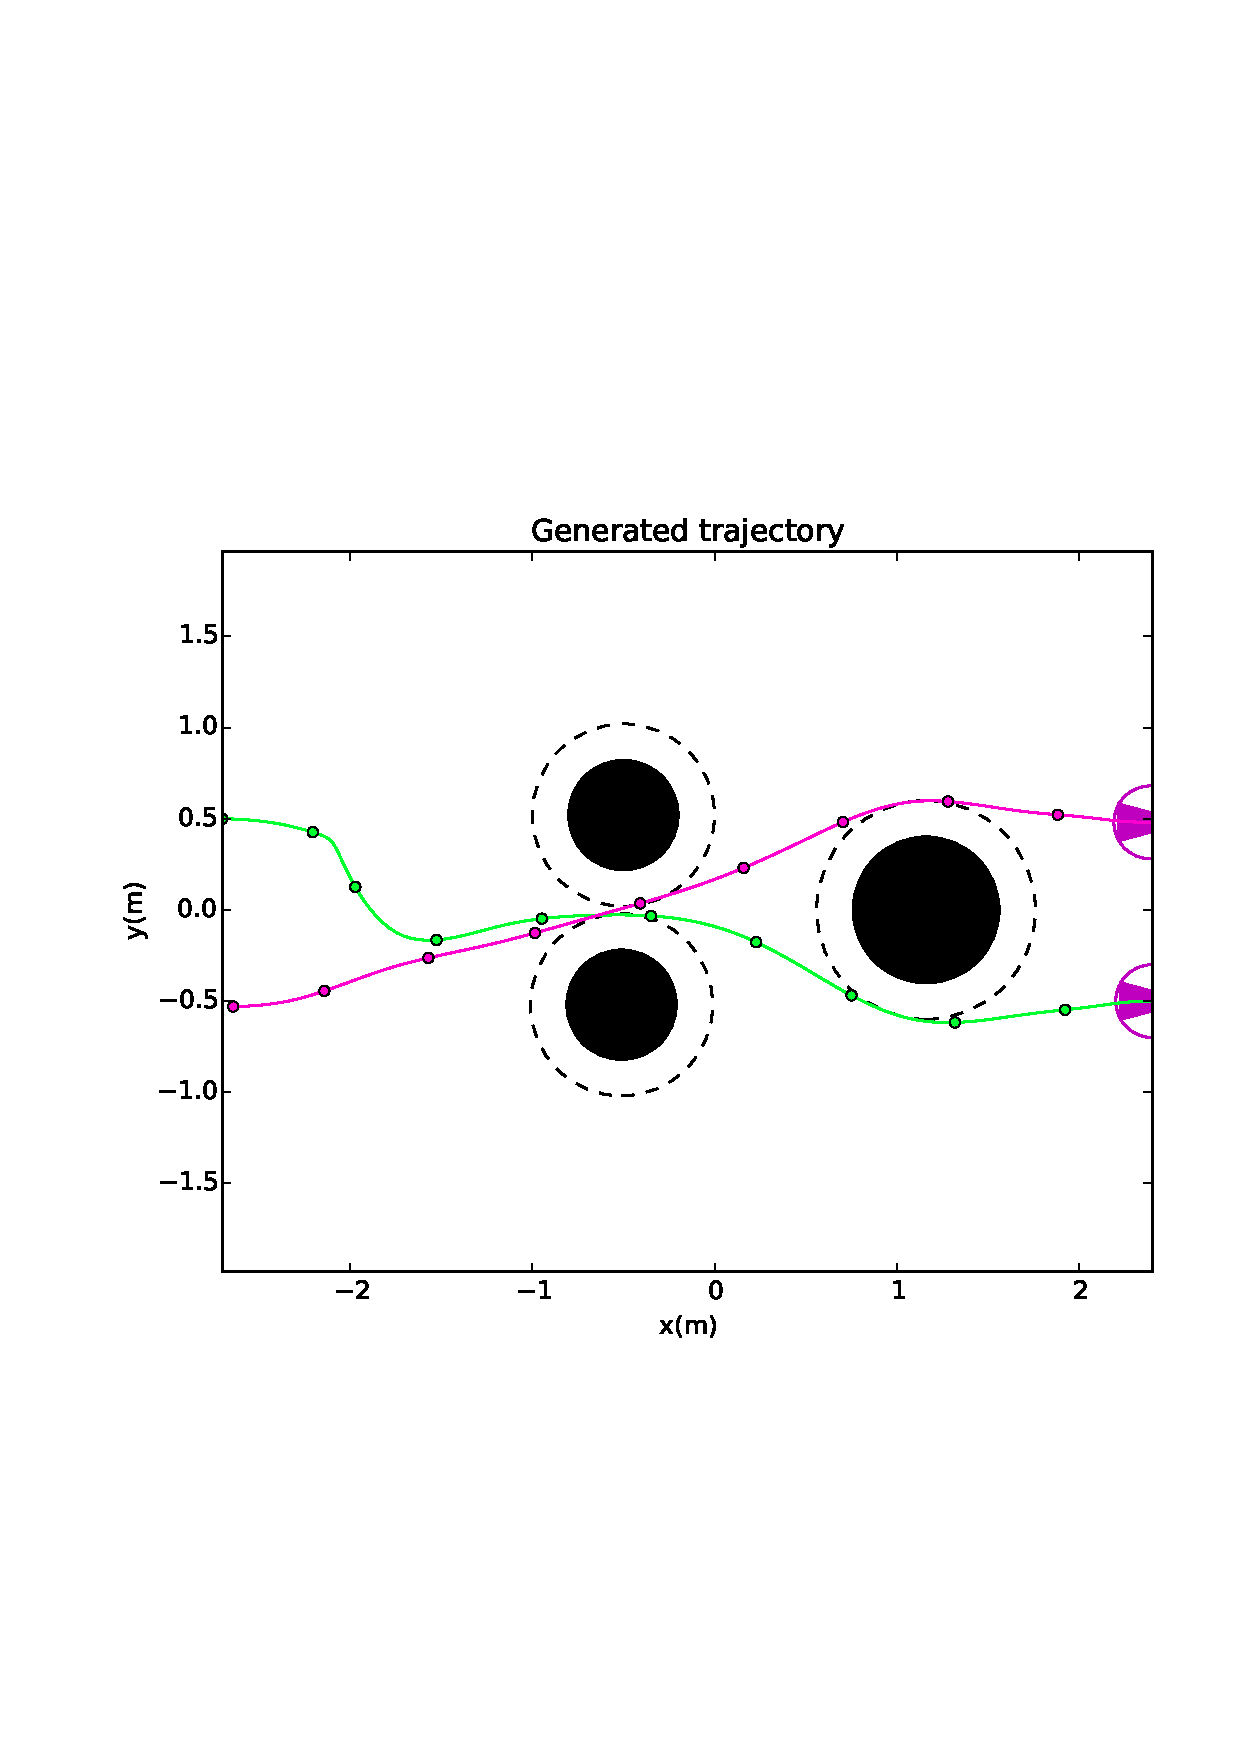
\includegraphics[width=\textwidth]{./images/pnc.png}
                \caption{Generated paths}\label{fig:pnc}
        \end{subfigure}
        ~ %add desired spacing between images, e. g. ~, \quad, \qquad, \hfill etc.
          %(or a blank line to force the subfigure onto a new line)
        \begin{subfigure}[b]{0.48\textwidth}
                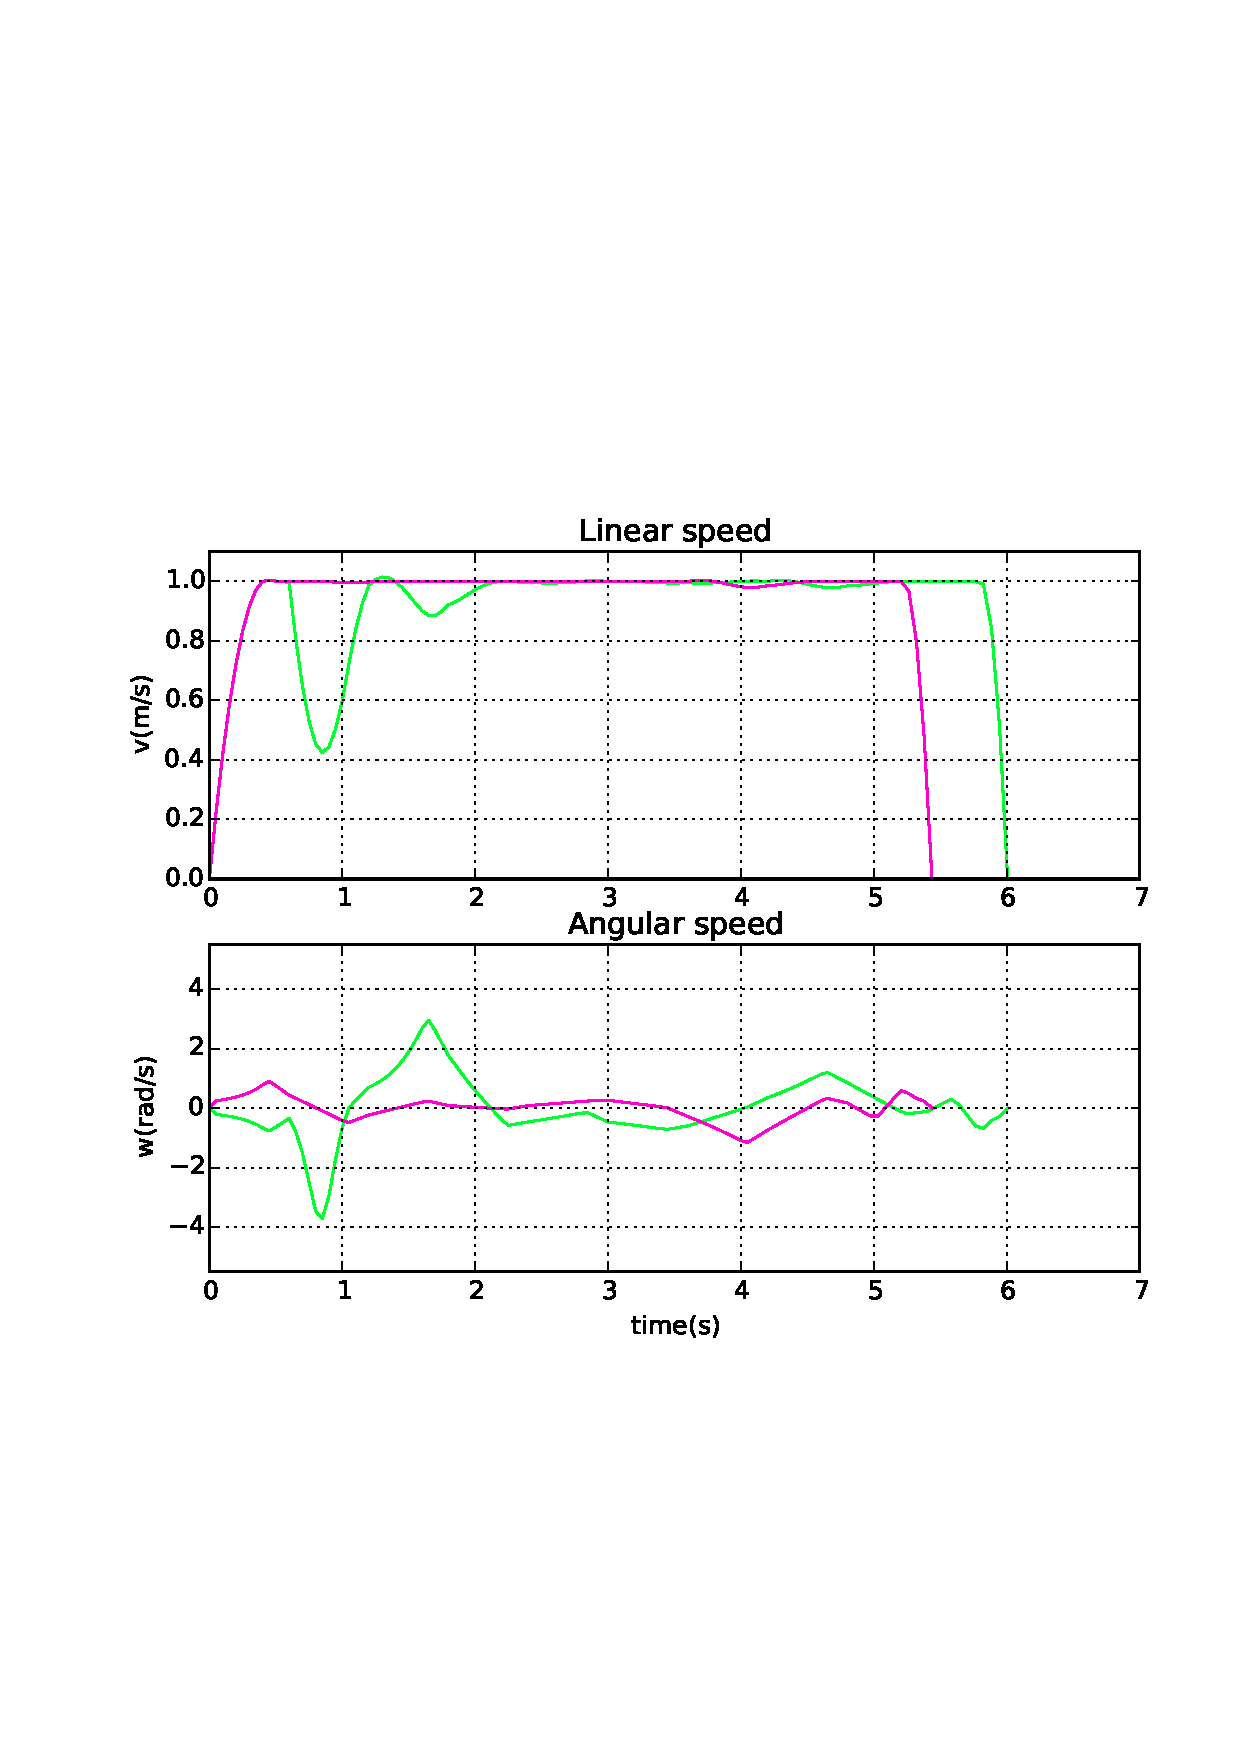
\includegraphics[width=\textwidth]{./images/vnc.png}
                \caption{Velocities}\label{fig:vnc}
        \end{subfigure}
        \caption{Multi-robot path generation with conflict handling.}\label{fig:nc}
\end{figure}

%\clearpage
\subsection{Analyzing the parameters impact on real-time feasibility and solution adequacy}

The performance of the motion planning algorithm previously presented depends on several parameters. For starters these parameters can be split into two groups. The \textbf{algorithm related} parameters and the \textbf{optimization solver related} ones. Among the former group the most important ones are:
\begin{itemize}
\item[$bullet$] The number of sample for time discretization ($N_s$);
\item[$\bullet$] The number of internal knots for the B-splines curves ($n_{knots}$);
\item[$\bullet$] The planning horizon for the sliding window ($T_p$);
\item[$\bullet$] The computation horizon ($T_c$).
\end{itemize}

The latter kind depends on the optimization solver adopted but since most of them are iterative methods it is common to have at least the two following parameters:
\begin{itemize}
\item[$\bullet$] Maximum number of iterations;
\item[$\bullet$] Stop condition.
\end{itemize}

The task of searching for a satisfactory set of parameters' values with regard to a performance metric (e.g. total time to complete the miss1ion) is quite laborious.

We attempted nevertheless to extract some quantitative knowledge about how these parameters impact the generated solution based on several simulations run with different parameters configurations. The main objective here is to be able to support the feasibility of a real-time motion planner based on this algorithm.

Omitting some details about the simulations conditions we present one of the many data used in our analyze in the figures~\ref{fig:uni3} and \ref{fig:r3}. Figure~\ref{fig:r3} shows the solution (path and velocities) for one of the scenarios that were simulated for a given set of parameters listed in the table~\ref{tab:s3param}. Keeping the scenario and varying the parameters we were able to plot the charts on figure \ref{fig:uni3}. We can notice an impact of the number of samples ($N_s$) and number of non-null internal knots ($n_{knots}$) on the \textit{maximum computation time}/$T_c$ ratio. The greater the $n_{knots}$ or the $N_s$ the greater is the \textit{maximum computation time}/$T_c$. This behavior is the one expected since the number of constraints and the number of arguments for the cost function to be minimized depend on these two parameters respectively. Keep in mind that the \textit{maximum computation time}/$T_c$ ratio has to be inferior to one so real-time planning is possible.

We were also able to characterize the influence of the number of obstacles seen at once on the computation time and path quality. As expected the computation time increases with the number of obstacles seen at once.

Finally we proposed some metric to characterize the adequacy of a found solution based on the total time spend going from the initial to the final pose and on the robot to the obstacles distance.

%INFO:R0: TOT: 7.57429378065
%INFO:R0: NSE: 15
%INFO:R0: FIR: 1.07032418251
%INFO:R0: LAS: 0.402824163437
%INFO:R0: LMA: 1
%INFO:R0: MAX: 0.243094921112
%INFO:R0: MIN: 0.0298509597778
%INFO:R0: AVG: 0.156346522845
%INFO:R0: RMP: 0.506447752317
%INFO:R0: RMG: 0.83921700716
%p_3_0.48_2.4_11_4_0.001_15_40_20_5.0_0.1_3.0_0.5_1.0_10.0


\begin{table}[!h]
\caption {Motion planner main parameters} \label{tab:s3param}
\begin{center}
\begin{tabular}{|c|c|}
\hline
$T_p$ & 2.40 s\\
\hline 
$T_c$ & 0.48 s\\
\hline 
$N_s$ & 11\\
\hline 
$n_{knots}$ & 4\\
\hline
$v_{max}$ & $1.00\ \mathrm{m/s}$\\
\hline
$\omega_{max}$ & $5.00\ \mathrm{rad/s}$\\
\hline
$q_{inital}$ & $[-0.05\ 0.00\ \pi/2]^T$\\
\hline
$q_{final}$ & $[0.10\ 7.00\ \pi/2]^T$\\
\hline
$u_{final}$ & $[0.00\ 0.00]^T$\\
\hline
$u_{final}$ & $[0.00\ 0.00]^T$\\
\hline
$O_0$ & $[0.55\ 1.91\ 0.31]$\\
\hline
$O_1$ & $[-0.08\ 3.65\ 0.32]$\\
\hline
$O_2$ & $[0.38\ 4.65\ 0.16]$\\
\hline
\end{tabular}
\end{center}
\end{table}

\begin{figure}[!h]
        \centering
        ~ %add desired spacing between images, e. g. ~, \quad, \qquad, \hfill etc.
          %(or a blank line to force the subfigure onto a new line)
        \begin{subfigure}[b]{0.48\textwidth}
                \includegraphics[width=\textwidth]{./images/realtime/sim_results/p_3_0.48_2.4_11_4_0.001_15_40_20_5.0_0.1_3.0_0.5_1.0_10.0/multirobot-path.png}
                \caption{Robot's path.}\label{fig:rpath}
        \end{subfigure}
        ~ %add desired spacing between images, e. g. ~, \quad, \qquad, \hfill etc.
          %(or a blank line to force the subfigure onto a new line)
        \begin{subfigure}[b]{0.48\textwidth}
		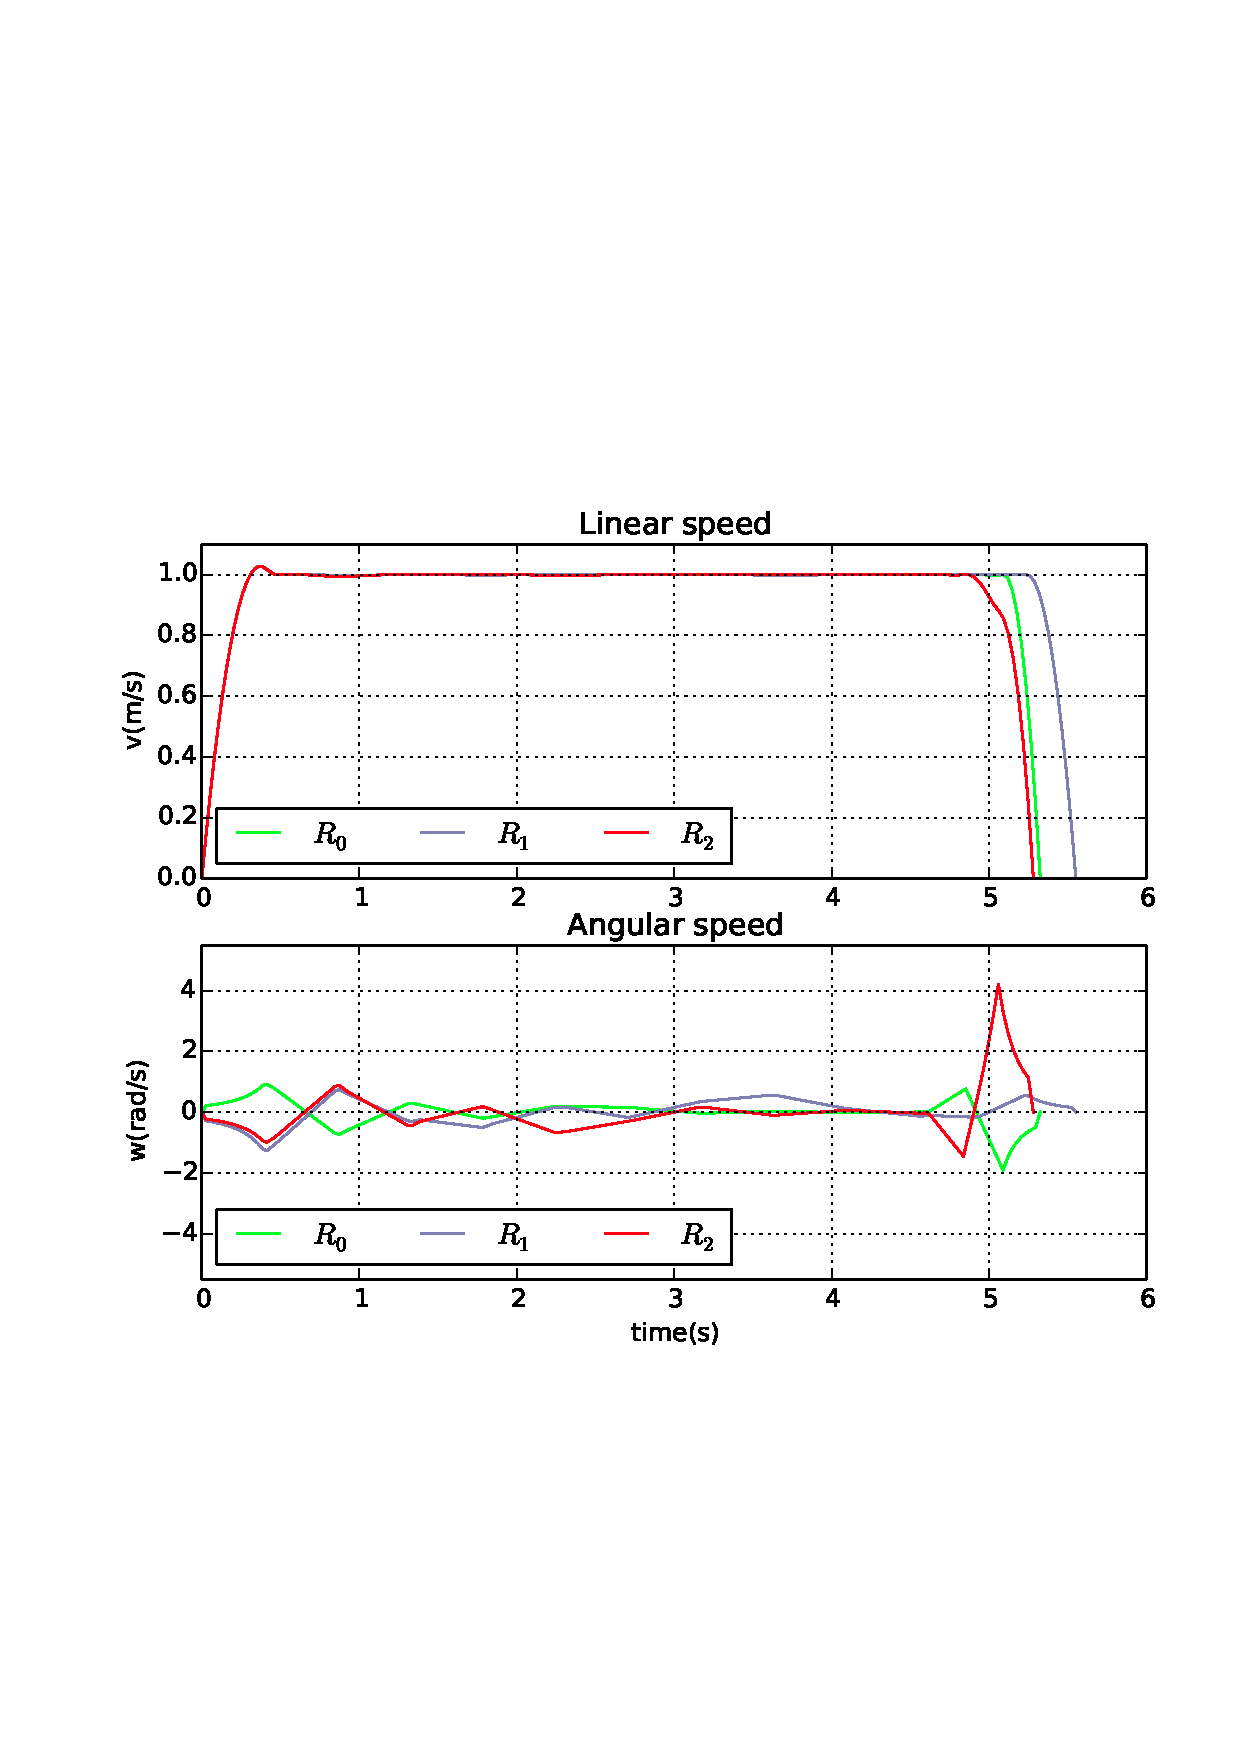
\includegraphics[width=\textwidth]{./images/realtime/sim_results/p_3_0.48_2.4_11_4_0.001_15_40_20_5.0_0.1_3.0_0.5_1.0_10.0/multirobot-vw.png}
                \caption{Robot's input.}\label{fig:rinput}
        \end{subfigure}
        \caption{Three obstacles scenario simulation example where the \textit{maximum computation time} was about 84\% of $T_c$ and the mission total time equals to $7.57\ s$.}\label{fig:r3}
\end{figure}

\begin{figure}[!h]
        \centering
        ~ %add desired spacing between images, e. g. ~, \quad, \qquad, \hfill etc.
          %(or a blank line to force the subfigure onto a new line)
        \begin{subfigure}[b]{0.48\textwidth}
                \includegraphics[width=\textwidth]{./images/realtime/Scenario_3__N_knots_4/mcttc-tctp.eps}
                \caption{Four internal knots. Average variance between lines is $1.047\times 10^{-2}$}\label{fig:uni34}
        \end{subfigure}
        
        ~ %add desired spacing between images, e. g. ~, \quad, \qquad, \hfill etc.
          %(or a blank line to force the subfigure onto a new line)
        \begin{subfigure}[b]{0.48\textwidth}
                \includegraphics[width=\textwidth]{./images/realtime/Scenario_3__N_knots_5/mcttc-tctp.eps}
                \caption{Five internal knots. Average variance between lines is $0.972\times 10^{-2}$}\label{fig:uni35}
        \end{subfigure}
        ~ %add desired spacing between images, e. g. ~, \quad, \qquad, \hfill etc.
          %(or a blank line to force the subfigure onto a new line)
        \begin{subfigure}[b]{0.48\textwidth}
                \includegraphics[width=\textwidth]{./images/realtime/Scenario_3__N_knots_6/mcttc-tctp.eps}
                \caption{Six internal knots. Average variance between lines is $0.587\times 10^{-2}$}\label{fig:uni36}
        \end{subfigure}
        \caption{Three obstacles scenario.}\label{fig:uni3}
\end{figure}


%\clearpage
\subsection{From Python to XDE simulator}

XDE is a physics simulation software environment fully developed by CEA-LIST that can handle a variety of physical aspects such as deformable bodies, multibody systems with kinematic constraints and contacts, and fluids.

Its utilization presents though some rough edges and a steep learning curve.

During the third month and beginning of the forth while producing the analysis referenced by the latest subsection we begin porting the implementation done in python to the XDE environment. 

The objective is to get much closer to a real physical system being able to implement dynamic behavior in the simulated environment which was previously neglected.
%For instance the obstacle detection can be based on real sensors models carrying uncertainties instead of assuming the absolute knowledge of an obstacle position as soon as it enters within the robot's detection radius.

% \todo[inline, color=green!40]{develop this article}
% \cite{Gao2006}
%\clearpage
\section{Discussions}
% \todo[inline, color=green!40]{Quels sont les avantages et inconvénients des techniques étudiées ? Quelles sont les limites de ces méthodes ? Quelles sont les hypothèses "cachées" que font ces méthodes ? ...}

We implemented and did some minors improvements on the solution proposed by \cite{Defoort2007a} and we gather a good understanding of the impact of the algorithm's parameters in the computation cost and in the quality of the solution.

% qualities
The implemented algorithm has the quality of dealing with multi-robot systems in a robust manner, handling collision as well as lost of communication conflicts without greatly increasing the computation time.

Besides, thanks to the reduction of the solution's search space by creating a parametric representation of the trajectory, this algorithm can respect real-time constraints for a multi-robot system evolving in a unknown environment where static obstacles are present.

The biggest drawback of this approach is how to choose a set of parameters (algorithm and numerical solver related) well adapted to a given scenario. We were able to identify the parameters that has a bigger influence on the solution adequacy and computation time. The number of samples ($N_s$) is the parameter that greatly impacts the computing time followed by the number of obstacles detected at once by the robot (defined by the detection radius and the obstacles positioning with respect to the robot). In the other hand, the solution adequacy depends highly on the $N_s/T_p$ ratio and on the number of internal knots of the B-spline representation $n_{knots}$.


%\clearpage
\section{Perspectives}
% \todo[inline, color=green!40]{Est-ce que le problème est résolu ? Quels axes d'amélioration peut-on envisager ?}

During the months to come we hope to finish the implementation of the C++ code in the XDE simulator and develop the current approach so it can address dynamic obstacles.

We plan to write a paper focusing on the impact of the algorithm's parameters on the computation cost and on the solution quality  for submitting to the International Workshop on On-line Decision-Making in Multi-Robot Coordination.


% Commands to include a figure:
% \begin{figure}
% \centering
% \includegraphics[width=0.5\textwidth]{frog.jpg}
% \caption{\label{fig:frog}This is a figure caption.}
% \end{figure}


% \bibliographystyle{unsrt}
%\clearpage
\selectlanguage{english}
%\nocite{*}
\bibliography{references}
\bibliographystyle{plain}


\end{document} to your LaTeX file where you want your
% title page.
%
%%%%%%%%%%%%%%%%%%%%%%%%%%%%%%%%%%%%%%%%%
%----------------------------------------------------------------------------------------
%	PACKAGES AND OTHER DOCUMENT CONFIGURATIONS
%----------------------------------------------------------------------------------------

\documentclass[12pt]{article}

\usepackage[T1]{fontenc}
\usepackage[utf8]{inputenc}
\usepackage[a4paper, left=2.8cm, right=2.0cm, top=3.0cm, bottom=3.0cm]{geometry}
\usepackage{graphicx}
\usepackage{amsmath, amssymb, amsfonts, amsthm}
\usepackage{float}
\usepackage{color}
\usepackage[english, french]{babel}
\usepackage{lipsum}
\usepackage{float}
%\usepackage{makeidx}
\usepackage{setspace}
\usepackage{url}
\usepackage[table]{xcolor}
\usepackage[nottoc]{tocbibind}
\usepackage{parcolumns}
\usepackage{fancyhdr}
\usepackage{tikz}
\usepackage{caption}
\usepackage{subcaption}
% \usepackage[enable]{easy-todo}
\usepackage{xargs}
\usepackage[colorinlistoftodos,prependcaption,textsize=tiny]{todonotes}
\usepackage{soul}
\usepackage{epstopdf}

\newcommandx{\change}[2][1=]{\todo[linecolor=red,backgroundcolor=red!25,bordercolor=red,#1]{#2}}

\newtheorem{problem}{Problem}
\newtheorem{theorem}{Theorem}
\newtheorem{lemma}{Lemma}
\newtheorem{example}{Example}
\newtheorem{remark}{Remark}
\newtheorem{definition}{Definition}
\newtheorem{proposition}{Proposition}
\newtheorem{corollary}{Corollorary}
\newtheorem{conjecture}{Conjecture}
\newtheorem{idea}{Idea}

\title{PFE-WrittenReport}
\author{MENDES FILHO, José Magno}

\newcommand{\N}{\mathbb{N}}
\newcommand{\R}{\mathbb{R}}
\newcommand{\Z}{\mathbb{Z}}

\numberwithin{equation}{section}

\newenvironment{abstractpage}
  {\cleardoublepage\vspace*{\fill}\thispagestyle{empty}}
  {\vfill\cleardoublepage}
\newenvironment{Abstract}[1]
  {\bigskip\selectlanguage{#1}%
   \begin{center}\bfseries\abstractname\end{center}}
  {\par\bigskip}

\begin{document}

%=======%
% TITLE %
%=======%

\begin{titlepage}

\newcommand{\HRule}{\rule{\linewidth}{0.5mm}}
\center

% Logos
\begin{minipage}{0.32\textwidth}
%\begin{center}
\begin{flushleft}
	\includegraphics[height=4.0cm]{./images/logo_ensta.jpg}
\end{flushleft}
\end{minipage}
\begin{minipage}{0.32\textwidth}
\begin{center}
	\includegraphics[height=1.6cm]{./images/upmc.png}
\end{center}
\end{minipage}
\begin{minipage}{0.32\textwidth}
\begin{flushright}
	\includegraphics[height=2.7cm]{./images/cea.png}
\end{flushright}
\end{minipage}
\mbox{}\\[1.5cm]

\selectlanguage{french}

\textsc{\LARGE PFE - rapport mi-parcours}\\[0.3cm]
\textsc{\Large Robotique et Systèmes Embarqués}\\[0.3cm]
\Large{2014/2015}\\[0.6cm]

\selectlanguage{english}

{Réf : DIASI / 15-351 \hfill}

\HRule \\[0.2cm]
\Huge \textbf{Local Dynamic Path Planning for an Autonomous Forklift in Human Environment}\\[-0.2cm] % Title
\HRule \\[0.5cm]

\begin{center}
\textbf{\textcolor{red}{\Large{
Unclassified Report}\\[-0.4cm]% Classified
\large{Can be made public on the internet}
}}
\end{center}

\begin{minipage}{0.55\textwidth}
\begin{flushleft} \Large
\emph{Author:}\\
José Magno \textsc{Mendes Filho} \\[0.7cm] % Author
\end{flushleft}
\end{minipage}
~
\begin{minipage}{0.35\textwidth}
\begin{flushright} \Large
\mbox{}\\[0.4cm]
Promotion 2014
\end{flushright}
\end{minipage}\\[1.0cm]

\begin{minipage}{0.45\textwidth}
\begin{flushleft} \large
\emph{Supervisor - ENSTA:}\\
David \textsc{Filliat} % Tuteur ENSTA
\end{flushleft}
\end{minipage}
~
\begin{minipage}{0.45\textwidth}
\begin{flushright} \large
\emph{Supervisor - CEA:} \\
Éric \textsc{Lucet} % Tuteur Ailleurs
\end{flushright}
\end{minipage}\\[1.0cm]

\large{Internship from 05 Mars 2015 to 28 August 2015}\\[0.6cm]
\large{CEA LIST Digiteo Moulon\\ Bât. 660 91191 GIF-SUR-YVETTE Cedex, France}
\end{titlepage}
%\thispagestyle{empty}

%\onehalfspace
%\frontmatter
%\cleardoublepage

\pagestyle{fancy}
\fancyhead{}
%\fancyhead[LE,RO]{\rightmark} %section
\fancyhead[RE,LO]{\leftmark} %chapter
\fancyfoot{}
\cfoot{\textsc{Mendes Filho} José Magno - CEA\\\textcolor{red}{Unclassified - Can be made public on the internet}}
\fancyfoot[OR,EL]{\thepage}

% Pour cette synthèse, vous devez choisir un sujet et faire une courte bibliographie en choisissant au moins 3 articles scientifiques. Vous devez m'envoyer un rapport de 3 pages max synthétisant ces articles selon le plan suivant:
% - Introduction : quel est le problème ? dans quel contexte le trouve t'on ? quel est  l'utilité de savoir le résoudre ? ...
% - Etat de l'art : présentation rapide des techniques des articles étudiés, de leur points communs et de leur différences....
% - Discussion : Quels sont les avantages et inconvénients des techniques étudiées ? Quelles sont les limites de ces méthodes ? Quelles sont les hypothèses "cachées" que font ces méthodes ? ...
% - Perspectives : Est-ce que le problème est résolu ? Quels axes d'amélioration peut-on envisager ?

% \begin{abstract}
% Your abstract.
% \end{abstract}
\selectlanguage{english}
\section{Introduction}

% \todo[inline, color=green!40]{quel est le problème ? dans quel contexte le trouve t'on ? quel est  l'utilité de savoir le résoudre ?}

This document is meant to describe the work done until now as well as the partial results and the perspectives for my final year internship as an engineering student at ENSTA ParisTech and UPMC - Paris VI.

The first two months of this internship toke place at the "Unité Informatique et Ingénierie des Systèmes" at ENSTA under the supervision of David Filliat. After that, from May to the present I have been working at CEA LIST Digiteo Moulon under the supervision of Eric Lucet.

\subsection{Internship context}

The work developed during this internship falls within the context of an applied research project on automation of a forklift truck for the effective supply of assembly lines.

Thus, the mobile robot has to be able to evolve in a partially known, shared with humans environment while being efficient with respect to time and energy spend on its tasks and preserving the workers' safety.

\subsection{Objectives}

The main objective of this internship is to implement, test, evaluate and improve an experimental path planning algorithm presented in details in~\cite{Defoort2007a} with respect to its applicability to a scenario where autonomous forklift trucks and humans share the same environment. This experimental planning algorithm consists in planning the mobile robot's path by solving a direct trajectory optimization problem~\cite{betts1998survey} using B-splines for representing the system flat output~\cite{milam2003real}. 

As stated~\cite{Defoort2007a} this approach presents good advantages for multi-robots systems evolving in an uncertain environment with static obstacles over other solutions. For instance, analytic methods are inapplicable for nonholonomic systems in presence of obstacles. Cell decomposition methods have the downside of requiring a \textit{a priori} space modeling. The dynamic window approach does not seem flexible enough to be extended to a multi-robot system.

The two main challenges that may be confronted during this work is how to guarantee real-time property for our specific application and how to generalize the algorithm in order to account for humans, i.e. dynamic obstacles.

\clearpage
\section{Initial achievements}
\label{sec:etatdelart}

% \todo[inline, color=green!40]{présentation rapide des techniques des articles étudiés, de leur points communs et de leur différences....}

During the first two months of this work we focused in understanding and reproducing the trajectory generation algorithm presented in~\cite{Defoort2007a} going from a single robot global planning method to a multi-robot local real-time planning. During the third month we focused in the analysis of the impact of different parameters in the method performance and feasibility.

\subsection{Nonlinear programming problem (NLP)}

Firstly we studied how the path planning problem could be translated into a nonlinear programming problem by intelligently using the mobile robot's model flatness property and representing the trajectory by B-splines.

\subsubsection{Problem Formulation}

Let us briefly and without mathematical rigor present how the problem of finding a collision-free, optimized path for a mobile robot represented by a unicycle model can be written.

The equation~\ref{eq:unic} represents the unicycle kinematic model. Thanks to the flatness property it is possible to be only interested in planning a trajectory for the flat output variable $z$ where $z = [x,\ y]^T$.

\begin{equation}\label{eq:unic}
\begin{array}{c}
\dot{q} = \mathrm{f}(q, u) \Rightarrow\\
\left[\begin{array}{c}
\dot{x}\\
\dot{y}\\
\dot{\theta}
\end{array}\right]=
\left[\begin{array}{c}
v\cos(\theta)\\
v\sin(\theta)\\
w
\end{array}\right]
\end{array}    
\end{equation}

The equations \ref{eq:phi1}, \ref{eq:phi2} show how the state variables and control variables can be calculated from the flat output and its first $l^{th}$ derivatives. This way, whenever we need to retrieve the fundamental variables we can by means of these equations.

\begin{equation}\label{eq:phi1}
            \begin{array}{l}
            \varphi_1(z(t_k),\dotsc,z^{(l)}(t_k))=\\
            \left[\begin{array}{c}
            x\\
            y\\
            \theta
            \end{array}\right]
            \left[\begin{array}{c}
            z_1\\
            z_2\\
            \arctan(\dot{z}_2/\dot{z}_1)\\
            \end{array}\right]
            \end{array}
\end{equation}

\begin{equation}\label{eq:phi2}
\begin{array}{l}
            \varphi_2(z(t_k),\dotsc,z^{(l)}(t_k))=\\
            \left[\begin{array}{c}
            v\\
            \omega
            \end{array}\right]
            = \left[\begin{array}{c}
            \sqrt{\dot{z}_{1}^{2} + \dot{z}_{2}^{2}}\\
            \dfrac{\dot{z}_{1}\ddot{z}_{2} -
            \dot{z}_{2}\ddot{z}_{1}}{\dot{z}_{1}^{2}+\dot{z}_{2}^{2}}
            \end{array}\right]
            \end{array}
\end{equation}

%\begin{equation}\label{eq:phi3}
%\begin{array}{l}
%            \varphi_3(z(t_k),\dotsc,z^{(l)}(t_k))=\\
%            \left[\begin{array}{c}
%            \dot{v}\\
%            \dot{\omega}
%            \end{array}\right]
%            = \left[\begin{array}{c}
%            \frac{\partial}{\partial t}v\\
%            \frac{\partial}{\partial t}\omega
%            \end{array}\right]
%            = \left[\begin{array}{c}
%            \frac{\dot{z}_1\ddot{z}_1 + \dot{z}_2\ddot{z}_2}{\|\dot{z}\|}\\
%            \frac{(\ddot{z}_1\ddot{z}_2+ z^{(3)}_2\dot{z}_1 - (\ddot{z}_2\ddot{z}_1+z^{(3)}_1\dot{z}_2))\|\dot{z}\|^2- 2(\dot{z}_1\ddot{z}_2-\dot{z}_2\ddot{z}_1)\|\dot{z}\|\dot{v}}{\|\dot{z}\|^4}
%            \end{array}\right]
%            \end{array}
%\end{equation}

Now let us write the NPL problem that minimizes the square of the time spend (\ref{eq:objective}) to go from a $q_{initial}$ pose at a $u_{initial}$ velocity to a $q_{final}$ pose at a $u_{final}$ velocity, avoiding $M$ static obstacles represented by circles with radius $r_m$\footnote{the own robot geometry is here represented by a circle of radius $\rho$}, having velocities in an admissible velocity set denoted by $\mathcal{U}$.

\begin{equation}\label{eq:objective}
	\underset{(t_{final},C_0,\dotsc,C_{d+n_{knot}-2})}{\mathrm{min}} J = (t_{final}-t_{initial})^{2}
\end{equation}

under the following constraints $\forall k \in \{0,\dotsc,N_s -1\}$ and $\forall m \in {0,\dotsc,M-1}$:
\begin{equation}%\label{eq:sysr4}
\left\lbrace\begin{array}{lcl}
    \varphi_1(z(t_{initial}),\dotsc,z^{(l-1)}(t_{initial})) & = & q_{initial}\\
    \varphi_1(z(t_{final}),\dotsc,z^{(l-1)}(t_{final})) & = & q_{final}\\
    \varphi_2(z(t_{initial}),\dotsc,z^{(l)}(t_{initial})) & = & u_{initial}\\
    \varphi_2(z(t_{final}),\dotsc,z^{(l)}(t_{final}))& = & u_{final}\\
    \varphi_2(z(t_k),\dotsc,z^{(l)}(t_k)) &\in& \mathcal{U}\\
    d_{O_m}(t_k) &\geq& \rho + r_m,\quad \forall O_m \in \mathcal{Q}_{occupied}
\end{array}\right.
\end{equation}

\subsubsection{Implementation of the solution}

Once we were able to write the problem as above the subsequent step was to implement this planning method using some programming language. We kept in mind that a high level language provided with some NLP solver package would be preferable.

We decided to use Python language and the Scipy package. Within the Scipy module many minimization methods can be found. For this specific optimization problem, only the method SLSPQ was appropriate. It was the only one to handle constrained minimization where the constraints could be equations as well as inequations.

Since the SLSPQ is a local optimization method the first guess used for initializing the solver had an impact on the time of convergence as well as on the found solution. A bad first guess can prevent the solver for converging at all, as shown in the figure~\ref{fig:planning-sim-trajc}.

Besides the bad first guess we notice another problem that could cause the Scipy implementation of the SLSQP solver to not converge. A too big cost value for the objective function (for instance, for values greater then $10^6$) could also prevent the convergence of the solver.

\begin{figure}[!h]
	\centering
	\includegraphics[width=0.6\textwidth]{./images/planning-sim-trajc.png}
	\caption{Path resulting from a bad initialisation.\label{fig:planning-sim-trajc}}
\end{figure}

An initialization algorithm was then proposed along some changes in the objective function evaluation so better solutions could be achieved quicker.

The initialization algorithm is a simple one that interactively changes the positions of the B-splines control points in order to prevent the initial trajectory guess to pass between two obstacles that are too close together (distance inter-obstacle smaller than the robot diameter).

\subsection{Evolving from the previous NLP to the sliding window multi-robot decentralized approach}

Solving the problem as stated in the previous subsection is only worth considering as a base initial solution to our problem.
%We are interested here in a real-time local planner that evolves in a %partially known environment suited for a multi-robot fleet.

Following the work done in~\cite{Defoort2007a} we built over the first implementation so to have a strongly decentralized planner for multi-robot fleet that is collision-free with respect to the robots in the fleet as well as to static obstacles as before. This new approach was suitable for real-time implementation as well. We chose a strongly decentralized approach over a centralized one so no central supervisor is needed and so we can keep the computation complexity of solving the trajectory optimization problem close to the one in a single robot system.

Using a sliding window in time the new planner produced a "per robot" intended trajectory meant to be valid within a planning horizon that was locally optimal with respect to a new objective function and collision-free only with respected to the static obstacles.

The presence of other robots is taken into account in a second moment: the intended trajectory is updated after the robots involved in a possible future conflict exchange their intended trajectories so no conflict (collision or lost of communication) occur for the corrected new trajectory.

Figures \ref{fig:wc} and \ref{fig:nc} show two multi-robot local planning without and with collision handling.

\begin{figure}[!h]
        \centering
        ~ %add desired spacing between images, e. g. ~, \quad, \qquad, \hfill etc.
          %(or a blank line to force the subfigure onto a new line)
        \begin{subfigure}[b]{0.48\textwidth}
                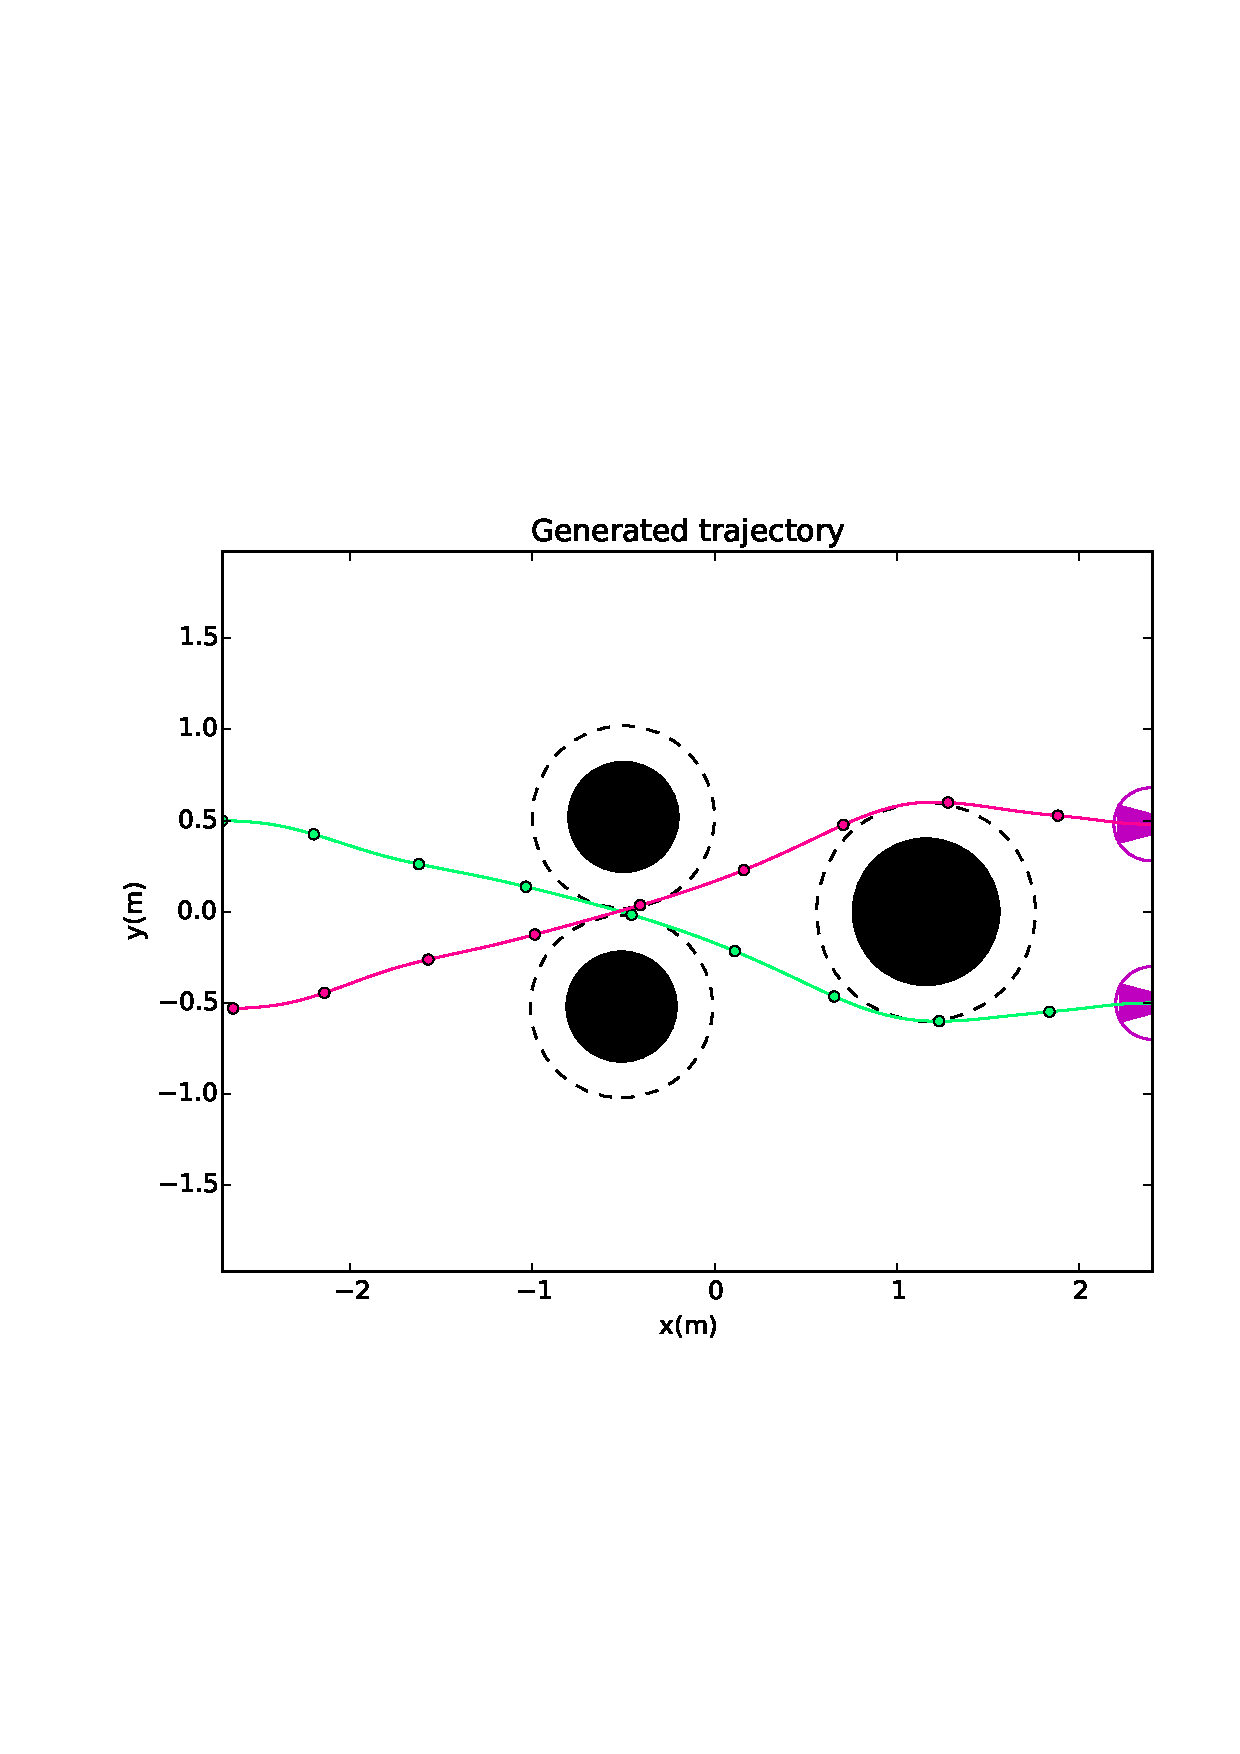
\includegraphics[width=\textwidth]{./images/pwc.png}
                \caption{Generated paths}\label{fig:pwc}
        \end{subfigure}
        ~ %add desired spacing between images, e. g. ~, \quad, \qquad, \hfill etc.
          %(or a blank line to force the subfigure onto a new line)
        \begin{subfigure}[b]{0.48\textwidth}
                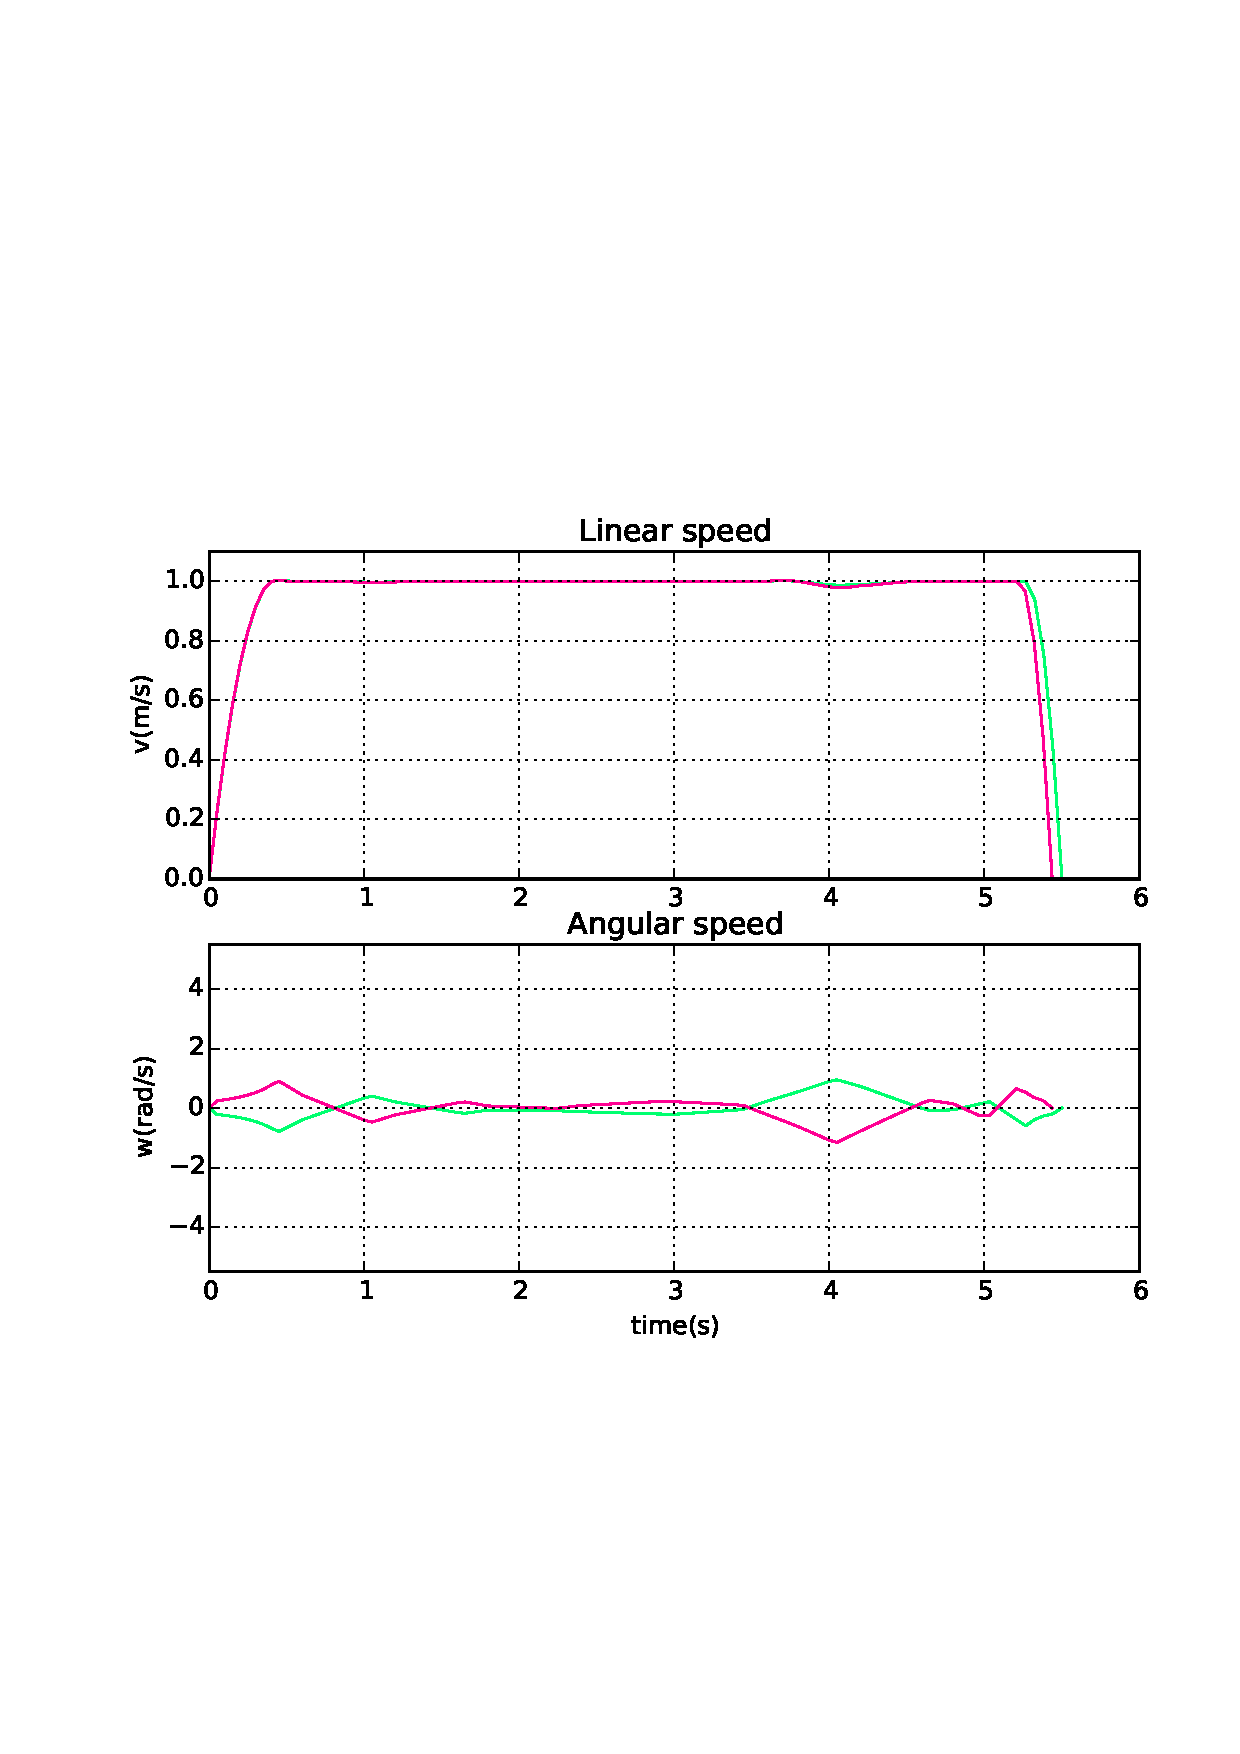
\includegraphics[width=\textwidth]{./images/vwc.png}
                \caption{Velocities}\label{fig:vwc}
        \end{subfigure}
        \caption{Multi-robot path generation without conflict handling.}\label{fig:wc}
\end{figure}

\begin{figure}[!h]
        \centering
        ~ %add desired spacing between images, e. g. ~, \quad, \qquad, \hfill etc.
          %(or a blank line to force the subfigure onto a new line)
        \begin{subfigure}[b]{0.48\textwidth}
                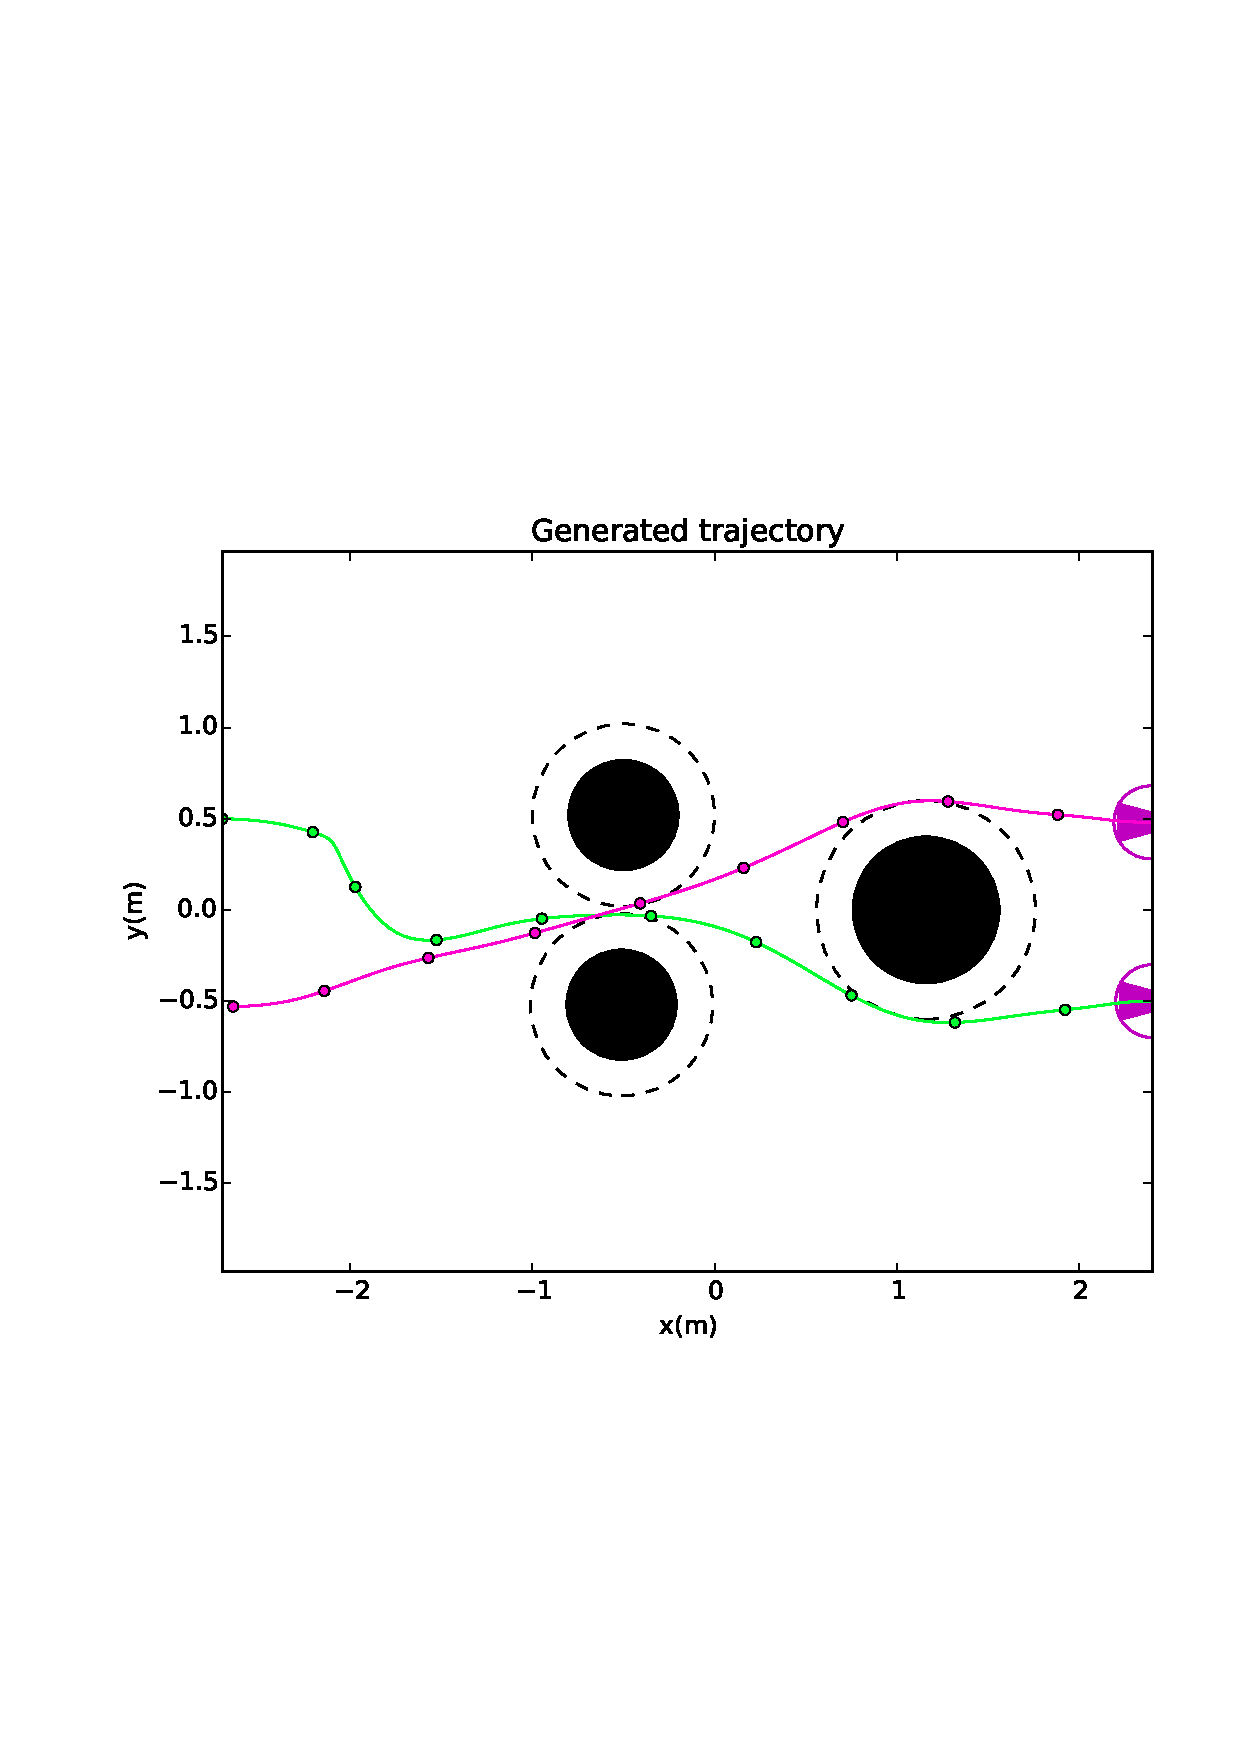
\includegraphics[width=\textwidth]{./images/pnc.png}
                \caption{Generated paths}\label{fig:pnc}
        \end{subfigure}
        ~ %add desired spacing between images, e. g. ~, \quad, \qquad, \hfill etc.
          %(or a blank line to force the subfigure onto a new line)
        \begin{subfigure}[b]{0.48\textwidth}
                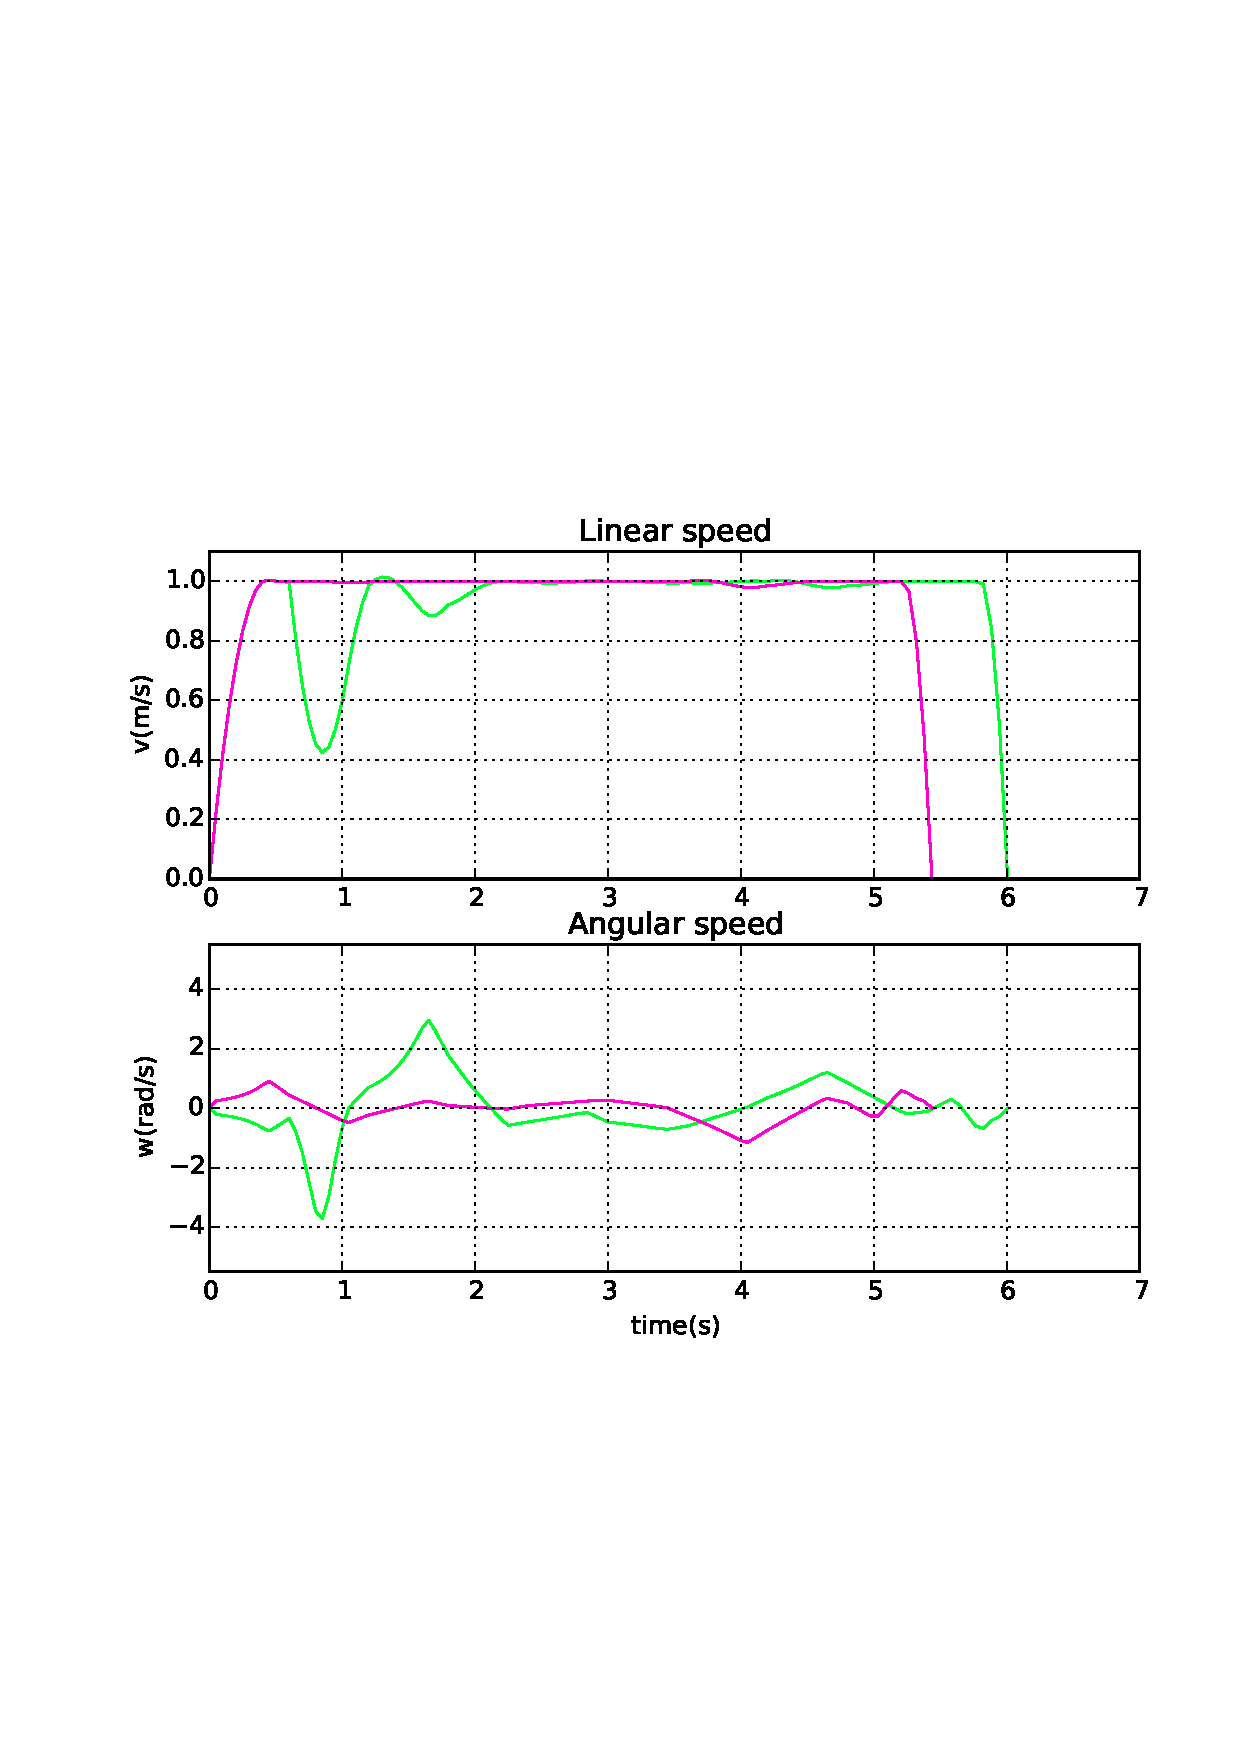
\includegraphics[width=\textwidth]{./images/vnc.png}
                \caption{Velocities}\label{fig:vnc}
        \end{subfigure}
        \caption{Multi-robot path generation with conflict handling.}\label{fig:nc}
\end{figure}

%\clearpage
\subsection{Analyzing the parameters impact on real-time feasibility and solution adequacy}

The performance of the motion planning algorithm previously presented depends on several parameters. For starters these parameters can be split into two groups. The \textbf{algorithm related} parameters and the \textbf{optimization solver related} ones. Among the former group the most important ones are:
\begin{itemize}
\item[$bullet$] The number of sample for time discretization ($N_s$);
\item[$\bullet$] The number of internal knots for the B-splines curves ($n_{knots}$);
\item[$\bullet$] The planning horizon for the sliding window ($T_p$);
\item[$\bullet$] The computation horizon ($T_c$).
\end{itemize}

The latter kind depends on the optimization solver adopted but since most of them are iterative methods it is common to have at least the two following parameters:
\begin{itemize}
\item[$\bullet$] Maximum number of iterations;
\item[$\bullet$] Stop condition.
\end{itemize}

The task of searching for a satisfactory set of parameters' values with regard to a performance metric (e.g. total time to complete the miss1ion) is quite laborious.

We attempted nevertheless to extract some quantitative knowledge about how these parameters impact the generated solution based on several simulations run with different parameters configurations. The main objective here is to be able to support the feasibility of a real-time motion planner based on this algorithm.

Omitting some details about the simulations conditions we present one of the many data used in our analyze in the figures~\ref{fig:uni3} and \ref{fig:r3}. Figure~\ref{fig:r3} shows the solution (path and velocities) for one of the scenarios that were simulated for a given set of parameters listed in the table~\ref{tab:s3param}. Keeping the scenario and varying the parameters we were able to plot the charts on figure \ref{fig:uni3}. We can notice an impact of the number of samples ($N_s$) and number of non-null internal knots ($n_{knots}$) on the \textit{maximum computation time}/$T_c$ ratio. The greater the $n_{knots}$ or the $N_s$ the greater is the \textit{maximum computation time}/$T_c$. This behavior is the one expected since the number of constraints and the number of arguments for the cost function to be minimized depend on these two parameters respectively. Keep in mind that the \textit{maximum computation time}/$T_c$ ratio has to be inferior to one so real-time planning is possible.

We were also able to characterize the influence of the number of obstacles seen at once on the computation time and path quality. As expected the computation time increases with the number of obstacles seen at once.

Finally we proposed some metric to characterize the adequacy of a found solution based on the total time spend going from the initial to the final pose and on the robot to the obstacles distance.

%INFO:R0: TOT: 7.57429378065
%INFO:R0: NSE: 15
%INFO:R0: FIR: 1.07032418251
%INFO:R0: LAS: 0.402824163437
%INFO:R0: LMA: 1
%INFO:R0: MAX: 0.243094921112
%INFO:R0: MIN: 0.0298509597778
%INFO:R0: AVG: 0.156346522845
%INFO:R0: RMP: 0.506447752317
%INFO:R0: RMG: 0.83921700716
%p_3_0.48_2.4_11_4_0.001_15_40_20_5.0_0.1_3.0_0.5_1.0_10.0


\begin{table}[!h]
\caption {Motion planner main parameters} \label{tab:s3param}
\begin{center}
\begin{tabular}{|c|c|}
\hline
$T_p$ & 2.40 s\\
\hline 
$T_c$ & 0.48 s\\
\hline 
$N_s$ & 11\\
\hline 
$n_{knots}$ & 4\\
\hline
$v_{max}$ & $1.00\ \mathrm{m/s}$\\
\hline
$\omega_{max}$ & $5.00\ \mathrm{rad/s}$\\
\hline
$q_{inital}$ & $[-0.05\ 0.00\ \pi/2]^T$\\
\hline
$q_{final}$ & $[0.10\ 7.00\ \pi/2]^T$\\
\hline
$u_{final}$ & $[0.00\ 0.00]^T$\\
\hline
$u_{final}$ & $[0.00\ 0.00]^T$\\
\hline
$O_0$ & $[0.55\ 1.91\ 0.31]$\\
\hline
$O_1$ & $[-0.08\ 3.65\ 0.32]$\\
\hline
$O_2$ & $[0.38\ 4.65\ 0.16]$\\
\hline
\end{tabular}
\end{center}
\end{table}

\begin{figure}[!h]
        \centering
        ~ %add desired spacing between images, e. g. ~, \quad, \qquad, \hfill etc.
          %(or a blank line to force the subfigure onto a new line)
        \begin{subfigure}[b]{0.48\textwidth}
                \includegraphics[width=\textwidth]{./images/realtime/sim_results/p_3_0.48_2.4_11_4_0.001_15_40_20_5.0_0.1_3.0_0.5_1.0_10.0/multirobot-path.png}
                \caption{Robot's path.}\label{fig:rpath}
        \end{subfigure}
        ~ %add desired spacing between images, e. g. ~, \quad, \qquad, \hfill etc.
          %(or a blank line to force the subfigure onto a new line)
        \begin{subfigure}[b]{0.48\textwidth}
		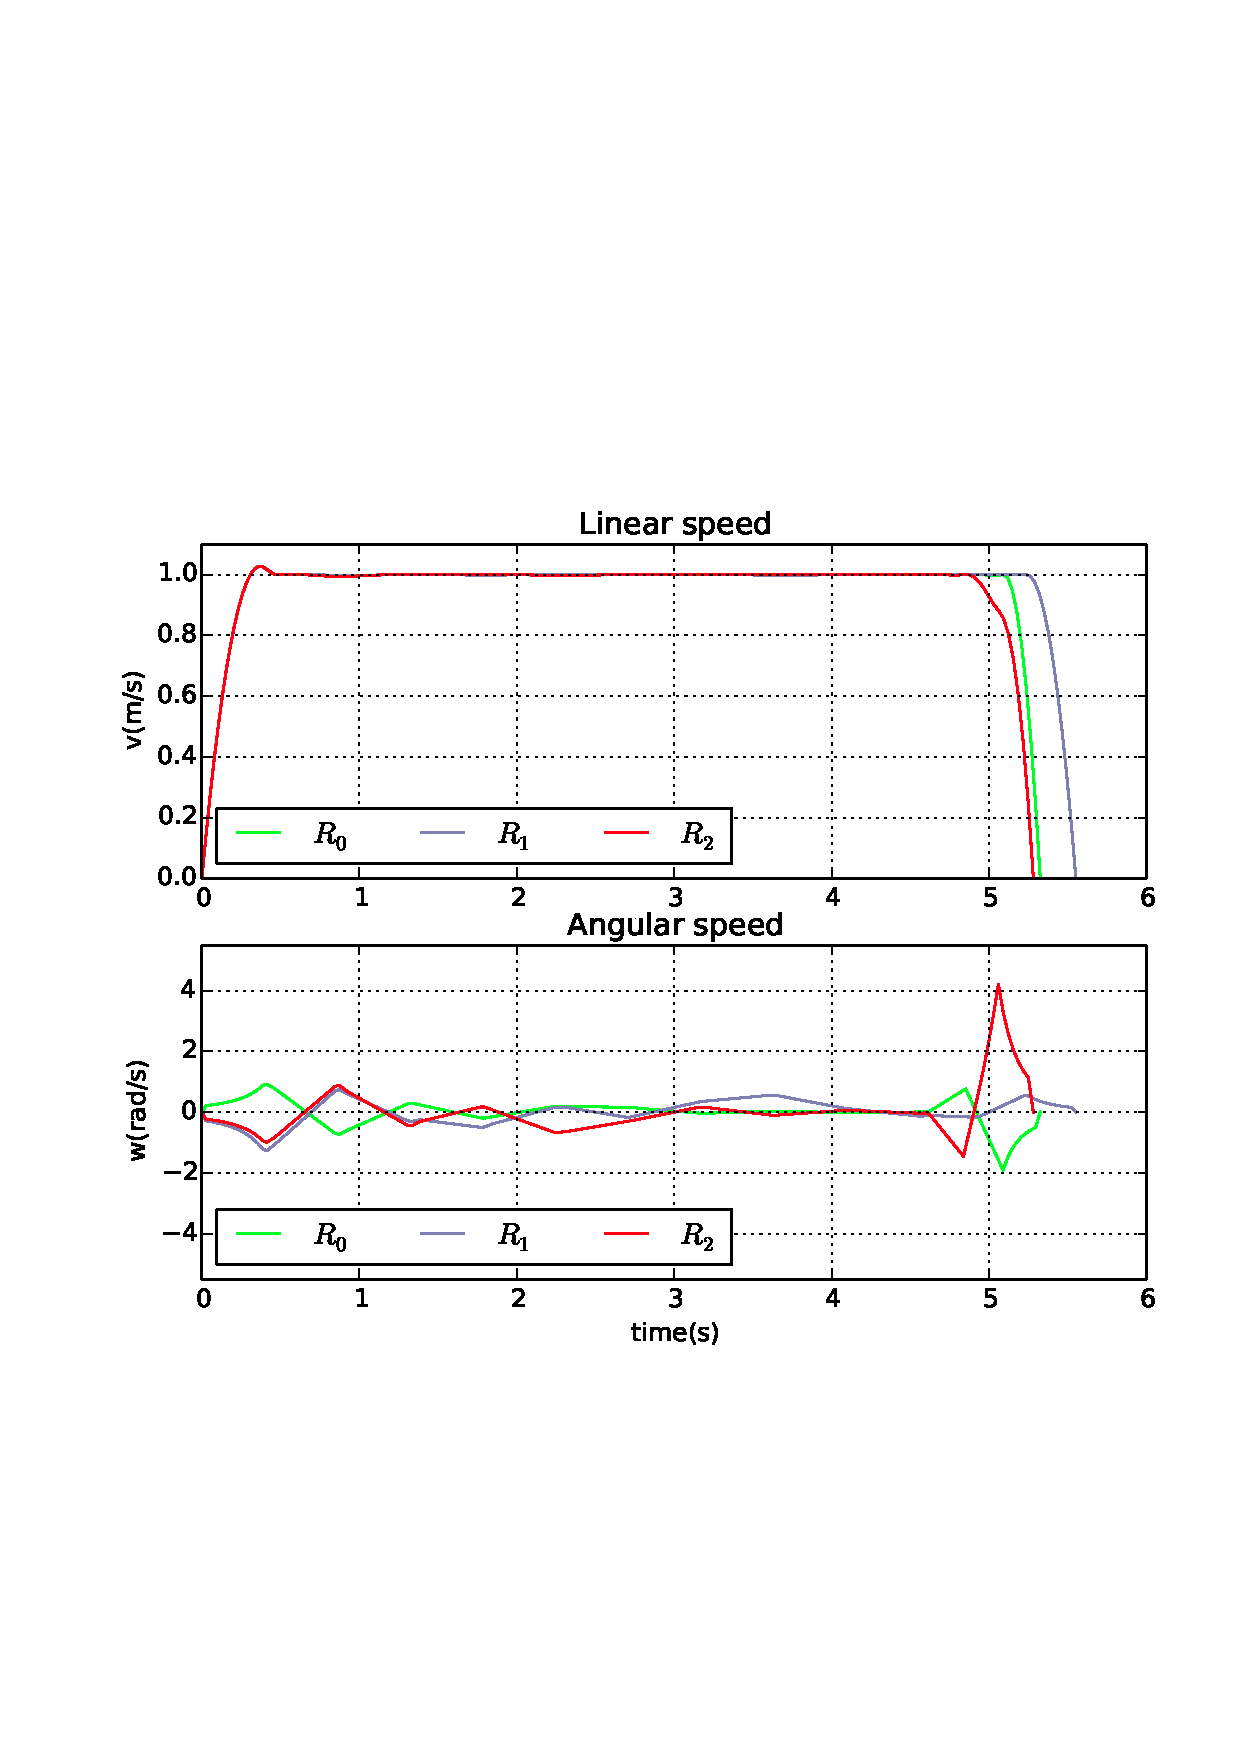
\includegraphics[width=\textwidth]{./images/realtime/sim_results/p_3_0.48_2.4_11_4_0.001_15_40_20_5.0_0.1_3.0_0.5_1.0_10.0/multirobot-vw.png}
                \caption{Robot's input.}\label{fig:rinput}
        \end{subfigure}
        \caption{Three obstacles scenario simulation example where the \textit{maximum computation time} was about 84\% of $T_c$ and the mission total time equals to $7.57\ s$.}\label{fig:r3}
\end{figure}

\begin{figure}[!h]
        \centering
        ~ %add desired spacing between images, e. g. ~, \quad, \qquad, \hfill etc.
          %(or a blank line to force the subfigure onto a new line)
        \begin{subfigure}[b]{0.48\textwidth}
                \includegraphics[width=\textwidth]{./images/realtime/Scenario_3__N_knots_4/mcttc-tctp.eps}
                \caption{Four internal knots. Average variance between lines is $1.047\times 10^{-2}$}\label{fig:uni34}
        \end{subfigure}
        
        ~ %add desired spacing between images, e. g. ~, \quad, \qquad, \hfill etc.
          %(or a blank line to force the subfigure onto a new line)
        \begin{subfigure}[b]{0.48\textwidth}
                \includegraphics[width=\textwidth]{./images/realtime/Scenario_3__N_knots_5/mcttc-tctp.eps}
                \caption{Five internal knots. Average variance between lines is $0.972\times 10^{-2}$}\label{fig:uni35}
        \end{subfigure}
        ~ %add desired spacing between images, e. g. ~, \quad, \qquad, \hfill etc.
          %(or a blank line to force the subfigure onto a new line)
        \begin{subfigure}[b]{0.48\textwidth}
                \includegraphics[width=\textwidth]{./images/realtime/Scenario_3__N_knots_6/mcttc-tctp.eps}
                \caption{Six internal knots. Average variance between lines is $0.587\times 10^{-2}$}\label{fig:uni36}
        \end{subfigure}
        \caption{Three obstacles scenario.}\label{fig:uni3}
\end{figure}


%\clearpage
\subsection{From Python to XDE simulator}

XDE is a physics simulation software environment fully developed by CEA-LIST that can handle a variety of physical aspects such as deformable bodies, multibody systems with kinematic constraints and contacts, and fluids.

Its utilization presents though some rough edges and a steep learning curve.

During the third month and beginning of the forth while producing the analysis referenced by the latest subsection we begin porting the implementation done in python to the XDE environment. 

The objective is to get much closer to a real physical system being able to implement dynamic behavior in the simulated environment which was previously neglected.
%For instance the obstacle detection can be based on real sensors models carrying uncertainties instead of assuming the absolute knowledge of an obstacle position as soon as it enters within the robot's detection radius.

% \todo[inline, color=green!40]{develop this article}
% \cite{Gao2006}
%\clearpage
\section{Discussions}
% \todo[inline, color=green!40]{Quels sont les avantages et inconvénients des techniques étudiées ? Quelles sont les limites de ces méthodes ? Quelles sont les hypothèses "cachées" que font ces méthodes ? ...}

We implemented and did some minors improvements on the solution proposed by \cite{Defoort2007a} and we gather a good understanding of the impact of the algorithm's parameters in the computation cost and in the quality of the solution.

% qualities
The implemented algorithm has the quality of dealing with multi-robot systems in a robust manner, handling collision as well as lost of communication conflicts without greatly increasing the computation time.

Besides, thanks to the reduction of the solution's search space by creating a parametric representation of the trajectory, this algorithm can respect real-time constraints for a multi-robot system evolving in a unknown environment where static obstacles are present.

The biggest drawback of this approach is how to choose a set of parameters (algorithm and numerical solver related) well adapted to a given scenario. We were able to identify the parameters that has a bigger influence on the solution adequacy and computation time. The number of samples ($N_s$) is the parameter that greatly impacts the computing time followed by the number of obstacles detected at once by the robot (defined by the detection radius and the obstacles positioning with respect to the robot). In the other hand, the solution adequacy depends highly on the $N_s/T_p$ ratio and on the number of internal knots of the B-spline representation $n_{knots}$.


%\clearpage
\section{Perspectives}
% \todo[inline, color=green!40]{Est-ce que le problème est résolu ? Quels axes d'amélioration peut-on envisager ?}

During the months to come we hope to finish the implementation of the C++ code in the XDE simulator and develop the current approach so it can address dynamic obstacles.

We plan to write a paper focusing on the impact of the algorithm's parameters on the computation cost and on the solution quality  for submitting to the International Workshop on On-line Decision-Making in Multi-Robot Coordination.


% Commands to include a figure:
% \begin{figure}
% \centering
% \includegraphics[width=0.5\textwidth]{frog.jpg}
% \caption{\label{fig:frog}This is a figure caption.}
% \end{figure}


% \bibliographystyle{unsrt}
%\clearpage
\selectlanguage{english}
%\nocite{*}
\bibliography{references}
\bibliographystyle{plain}


\end{document} to your LaTeX file where you want your
% title page.
%
%%%%%%%%%%%%%%%%%%%%%%%%%%%%%%%%%%%%%%%%%
%----------------------------------------------------------------------------------------
%	PACKAGES AND OTHER DOCUMENT CONFIGURATIONS
%----------------------------------------------------------------------------------------

\documentclass[12pt]{article}

\usepackage[T1]{fontenc}
\usepackage[utf8]{inputenc}
\usepackage[a4paper, left=2.8cm, right=2.0cm, top=3.0cm, bottom=3.0cm]{geometry}
\usepackage{graphicx}
\usepackage{amsmath, amssymb, amsfonts, amsthm}
\usepackage{float}
\usepackage{color}
\usepackage[english, french]{babel}
\usepackage{lipsum}
\usepackage{float}
%\usepackage{makeidx}
\usepackage{setspace}
\usepackage{url}
\usepackage[table]{xcolor}
\usepackage[nottoc]{tocbibind}
\usepackage{parcolumns}
\usepackage{fancyhdr}
\usepackage{tikz}
\usepackage{caption}
\usepackage{subcaption}
% \usepackage[enable]{easy-todo}
\usepackage{xargs}
\usepackage[colorinlistoftodos,prependcaption,textsize=tiny]{todonotes}
\usepackage{soul}
\usepackage{epstopdf}

\newcommandx{\change}[2][1=]{\todo[linecolor=red,backgroundcolor=red!25,bordercolor=red,#1]{#2}}

\newtheorem{problem}{Problem}
\newtheorem{theorem}{Theorem}
\newtheorem{lemma}{Lemma}
\newtheorem{example}{Example}
\newtheorem{remark}{Remark}
\newtheorem{definition}{Definition}
\newtheorem{proposition}{Proposition}
\newtheorem{corollary}{Corollorary}
\newtheorem{conjecture}{Conjecture}
\newtheorem{idea}{Idea}

\title{PFE-WrittenReport}
\author{MENDES FILHO, José Magno}

\newcommand{\N}{\mathbb{N}}
\newcommand{\R}{\mathbb{R}}
\newcommand{\Z}{\mathbb{Z}}

\numberwithin{equation}{section}

\newenvironment{abstractpage}
  {\cleardoublepage\vspace*{\fill}\thispagestyle{empty}}
  {\vfill\cleardoublepage}
\newenvironment{Abstract}[1]
  {\bigskip\selectlanguage{#1}%
   \begin{center}\bfseries\abstractname\end{center}}
  {\par\bigskip}

\begin{document}

%=======%
% TITLE %
%=======%

\begin{titlepage}

\newcommand{\HRule}{\rule{\linewidth}{0.5mm}}
\center

% Logos
\begin{minipage}{0.32\textwidth}
%\begin{center}
\begin{flushleft}
	\includegraphics[height=4.0cm]{./images/logo_ensta.jpg}
\end{flushleft}
\end{minipage}
\begin{minipage}{0.32\textwidth}
\begin{center}
	\includegraphics[height=1.6cm]{./images/upmc.png}
\end{center}
\end{minipage}
\begin{minipage}{0.32\textwidth}
\begin{flushright}
	\includegraphics[height=2.7cm]{./images/cea.png}
\end{flushright}
\end{minipage}
\mbox{}\\[1.5cm]

\selectlanguage{french}

\textsc{\LARGE PFE - rapport mi-parcours}\\[0.3cm]
\textsc{\Large Robotique et Systèmes Embarqués}\\[0.3cm]
\Large{2014/2015}\\[0.6cm]

\selectlanguage{english}

{Réf : DIASI / 15-351 \hfill}

\HRule \\[0.2cm]
\Huge \textbf{Local Dynamic Motion Planning for an Autonomous Forklift in Human Environment}\\[-0.2cm] % Title
\HRule \\[0.5cm]

\begin{center}
\textbf{\textcolor{red}{\Large{
Unclassified Report}\\[-0.4cm]% Classified
\large{Can be made public on the internet}
}}
\end{center}

\begin{minipage}{0.55\textwidth}
\begin{flushleft} \Large
\emph{Author:}\\
José Magno \textsc{Mendes Filho} \\[0.7cm] % Author
\end{flushleft}
\end{minipage}
~
\begin{minipage}{0.35\textwidth}
\begin{flushright} \Large
\mbox{}\\[0.4cm]
Promotion 2014
\end{flushright}
\end{minipage}\\[1.0cm]

\begin{minipage}{0.45\textwidth}
\begin{flushleft} \large
\emph{Supervisor - ENSTA:}\\
David \textsc{Filliat} % Tuteur ENSTA
\end{flushleft}
\end{minipage}
~
\begin{minipage}{0.45\textwidth}
\begin{flushright} \large
\emph{Supervisor - CEA:} \\
Éric \textsc{Lucet} % Tuteur Ailleurs
\end{flushright}
\end{minipage}\\[1.0cm]

\large{Internship from 05 Mars 2015 to 28 August 2015}\\[0.6cm]
\large{CEA LIST Digiteo Moulon\\ Bât. 660 91191 GIF-SUR-YVETTE Cedex, France}
\end{titlepage}
%\thispagestyle{empty}

%\onehalfspace
%\frontmatter
%\cleardoublepage

\pagestyle{fancy}
\fancyhead{}
%\fancyhead[LE,RO]{\rightmark} %section
\fancyhead[RE,LO]{\leftmark} %chapter
\fancyfoot{}
\cfoot{\textsc{Mendes Filho} José Magno - CEA\\\textcolor{red}{Unclassified - Can be made public on the internet}}
\fancyfoot[OR,EL]{\thepage}

% Pour cette synthèse, vous devez choisir un sujet et faire une courte bibliographie en choisissant au moins 3 articles scientifiques. Vous devez m'envoyer un rapport de 3 pages max synthétisant ces articles selon le plan suivant:
% - Introduction : quel est le problème ? dans quel contexte le trouve t'on ? quel est  l'utilité de savoir le résoudre ? ...
% - Etat de l'art : présentation rapide des techniques des articles étudiés, de leur points communs et de leur différences....
% - Discussion : Quels sont les avantages et inconvénients des techniques étudiées ? Quelles sont les limites de ces méthodes ? Quelles sont les hypothèses "cachées" que font ces méthodes ? ...
% - Perspectives : Est-ce que le problème est résolu ? Quels axes d'amélioration peut-on envisager ?

% \begin{abstract}
% Your abstract.
% \end{abstract}
\selectlanguage{english}
\section{Introduction}

% \todo[inline, color=green!40]{quel est le problème ? dans quel contexte le trouve t'on ? quel est  l'utilité de savoir le résoudre ?}

The main objective of this internship is to implement, test, evaluate and improve an experimental path planning algorithm for mobile robots with respect to its applicability to a scenario where autonomous forklift trucks and humans share the same environment.

The base planning algorithm is presented in details in~\cite{Defoort2007a}.
It consists in planning the mobile robot's path by solving a direct trajectory optimization problem~\cite{betts1998survey} using B-splines for representing the system flat output~\cite{milam2003real}.

This approach have presented good results for multirobots systems evolving in an uncertain environment with static obstacles.

The main challenge that may be confronted during this work is how to generalize the algorithm in order to account for humans, i.e. dynamic obstacles.
%\clearpage
\section{Initial achievements}
\label{sec:etatdelart}

% \todo[inline, color=green!40]{présentation rapide des techniques des articles étudiés, de leur points communs et de leur différences....}

During the first two months of this work we focused in understanding and reproducing the trajectory generation algorithm presented in~\cite{Defoort2007a} going from a single robot global planning method to a multirobot local real-time planning. During the third month we focused in the analysis of the impact of different parameters in the method performance and feasibility.

\subsection{Nonlinear programming problem (NLP)}

Firstly we studied how the path planning problem could be translated in a nonlinear programming problem by intelligently using the mobile robot's model flatness property and representing the trajectory by B-splines.

Let us briefly and without mathematical rigor present how the problem of finding a collision-free, optimized path for a mobile robot represented by a unicycle model can be written.

The equation~\ref{eq:unic} represents the unicycle kinematic model. Thanks to the flatness property it is possible to be only interested in planning a trajectory for the flat output variable $z$ where $z = [x,\ y]^T$.

\begin{equation}\label{eq:unic}
\begin{array}{c}
\dot{q} = \mathrm{f}(q, u) \Rightarrow\\
\left[\begin{array}{c}
\dot{x}\\
\dot{y}\\
\dot{\theta}
\end{array}\right]=
\left[\begin{array}{c}
v\cos(\theta)\\
v\sin(\theta)\\
w
\end{array}\right]
\end{array}    
\end{equation}

The equations \ref{eq:phi1}, \ref{eq:phi2} show how the state variables and control variables can be calculated from the flat output and its first $l^{th}$ derivatives. This way, whenever we need to retrieve the fundamental variables we can by means of these equations.

\begin{equation}\label{eq:phi1}
            \begin{array}{l}
            \varphi_1(z(t_k),\dotsc,z^{(l)}(t_k))=\\
            \left[\begin{array}{c}
            x\\
            y\\
            \theta
            \end{array}\right]
            \left[\begin{array}{c}
            z_1\\
            z_2\\
            \arctan(\dot{z}_2/\dot{z}_1)\\
            \end{array}\right]
            \end{array}
\end{equation}

\begin{equation}\label{eq:phi2}
\begin{array}{l}
            \varphi_2(z(t_k),\dotsc,z^{(l)}(t_k))=\\
            \left[\begin{array}{c}
            v\\
            \omega
            \end{array}\right]
            = \left[\begin{array}{c}
            \sqrt{\dot{z}_{1}^{2} + \dot{z}_{2}^{2}}\\
            \dfrac{\dot{z}_{1}\ddot{z}_{2} -
            \dot{z}_{2}\ddot{z}_{1}}{\dot{z}_{1}^{2}+\dot{z}_{2}^{2}}
            \end{array}\right]
            \end{array}
\end{equation}

%\begin{equation}\label{eq:phi3}
%\begin{array}{l}
%            \varphi_3(z(t_k),\dotsc,z^{(l)}(t_k))=\\
%            \left[\begin{array}{c}
%            \dot{v}\\
%            \dot{\omega}
%            \end{array}\right]
%            = \left[\begin{array}{c}
%            \frac{\partial}{\partial t}v\\
%            \frac{\partial}{\partial t}\omega
%            \end{array}\right]
%            = \left[\begin{array}{c}
%            \frac{\dot{z}_1\ddot{z}_1 + \dot{z}_2\ddot{z}_2}{\|\dot{z}\|}\\
%            \frac{(\ddot{z}_1\ddot{z}_2+ z^{(3)}_2\dot{z}_1 - (\ddot{z}_2\ddot{z}_1+z^{(3)}_1\dot{z}_2))\|\dot{z}\|^2- 2(\dot{z}_1\ddot{z}_2-\dot{z}_2\ddot{z}_1)\|\dot{z}\|\dot{v}}{\|\dot{z}\|^4}
%            \end{array}\right]
%            \end{array}
%\end{equation}

Now let us write the NPL problem that minimizes the square of the time spend (\ref{eq:objective}) to go from a $q_{initial}$ pose at a $u_{initial}$ velocity to a $q_{final}$ pose at a $u_{final}$ velocity, avoiding $M$ static obstacles represented by circles with radius $r_m$\footnote{the own robot geometry is here represented by a circle of radius $\rho$}, having velocities in an admissible velocity set denoted by $\mathcal{U}$.

\begin{equation}\label{eq:objective}
	\underset{(t_{final},C_0,\dotsc,C_{d+n_{knot}-2})}{\mathrm{min}} J = (t_{final}-t_{initial})^{2}
\end{equation}

under the following constraints $\forall k \in \{0,\dotsc,N_s -1\}$ and $\forall m \in {0,\dotsc,M-1}$:
\begin{equation}%\label{eq:sysr4}
\left\lbrace\begin{array}{lcl}
    \varphi_1(z(t_{initial}),\dotsc,z^{(l-1)}(t_{initial})) & = & q_{initial}\\
    \varphi_1(z(t_{final}),\dotsc,z^{(l-1)}(t_{final})) & = & q_{final}\\
    \varphi_2(z(t_{initial}),\dotsc,z^{(l)}(t_{initial})) & = & u_{initial}\\
    \varphi_2(z(t_{final}),\dotsc,z^{(l)}(t_{final}))& = & u_{final}\\
    \varphi_2(z(t_k),\dotsc,z^{(l)}(t_k)) &\in& \mathcal{U}\\
    d_{O_m}(t_k) &\geq& \rho + r_m,\quad \forall O_m \in \mathcal{Q}_{occupied}
\end{array}\right.
\end{equation}

Once we were able to write the problem as above the subsequent step was to implement this planning method using some programming language. We kept in mind that a high level language provided with some NLP solver package would be preferable.

We decided to use Python language and the Scipy package. Within the Scipy module many minimization methods can be found. For this specific optimization problem, only the method SLSPQ was appropriate. It was the only one to handle constrained minimization where the constraints could be equations as well as inequations.

Since the SLSPQ is a local optimization method the first guess used for initializing the solver had a impact on the time of convergence as well as on the found solution. A bad first guess can prevent the solver for converging at all as shown in the figure~\ref{fig:planning-sim-trajc}.

Besides the bad first guess we notice another problem that could cause the Scipy implementation of the SLSQP solver to not converge. A too big cost value for the objective function (for instance, for values greater then $10^6$) could also prevent the convergence of the solver.

\begin{figure}[!h]
	\centering
	\includegraphics[width=0.7\textwidth]{./images/planning-sim-trajc.png}
	\caption{Bad first guess.\label{fig:planning-sim-trajc}}
\end{figure}

A initialization algorithm was then proposed along some changes in the objective function evaluation so better solutions could be achieved quicker.

The initialization algorithm is a simple one that interactively changes the positions of the B-splines control points in order to prevent the initial trajectory guess to pass between two obstacles that are too close together (distance inter-obstacle smaller than the robot diameter).

\subsection{Evolving from the previous NLP to the sliding window multirobot decentralized approach}

Solving the problem as stated in the previous subsection is only worth considering as a base initial solution to our problem.
%We are interested here in a real-time local planner that evolves in a %partially known environment suited for a multirobot fleet.

Following the work done in~\cite{Defoort2007a} we built over the first implementation so to have a strongly decentralized planner for multirobot fleet that is collision-free with respect to the robots in the fleet as well as to static obstacles as before. This new approach was suitable for real-time implementation as well.

Using a sliding window in time the new planner produced a "per robot" intended trajectory meant to be valid within a planning horizon that was locally optimal with respect to a new objective function and collision-free only with respected to the static obstacles.

The presence of other robots is taken into account in a second moment: the intended trajectory is updated after the robots involved in a possible future conflict exchange their intended trajectories so no conflict (collision or lost of communication) occur for the corrected new trajectory.

Figures \ref{fig:wc} and \ref{fig:nc} show two multirobot local planning without and with collision handling.

\begin{figure}[!h]
        \centering
        ~ %add desired spacing between images, e. g. ~, \quad, \qquad, \hfill etc.
          %(or a blank line to force the subfigure onto a new line)
        \begin{subfigure}[b]{0.48\textwidth}
                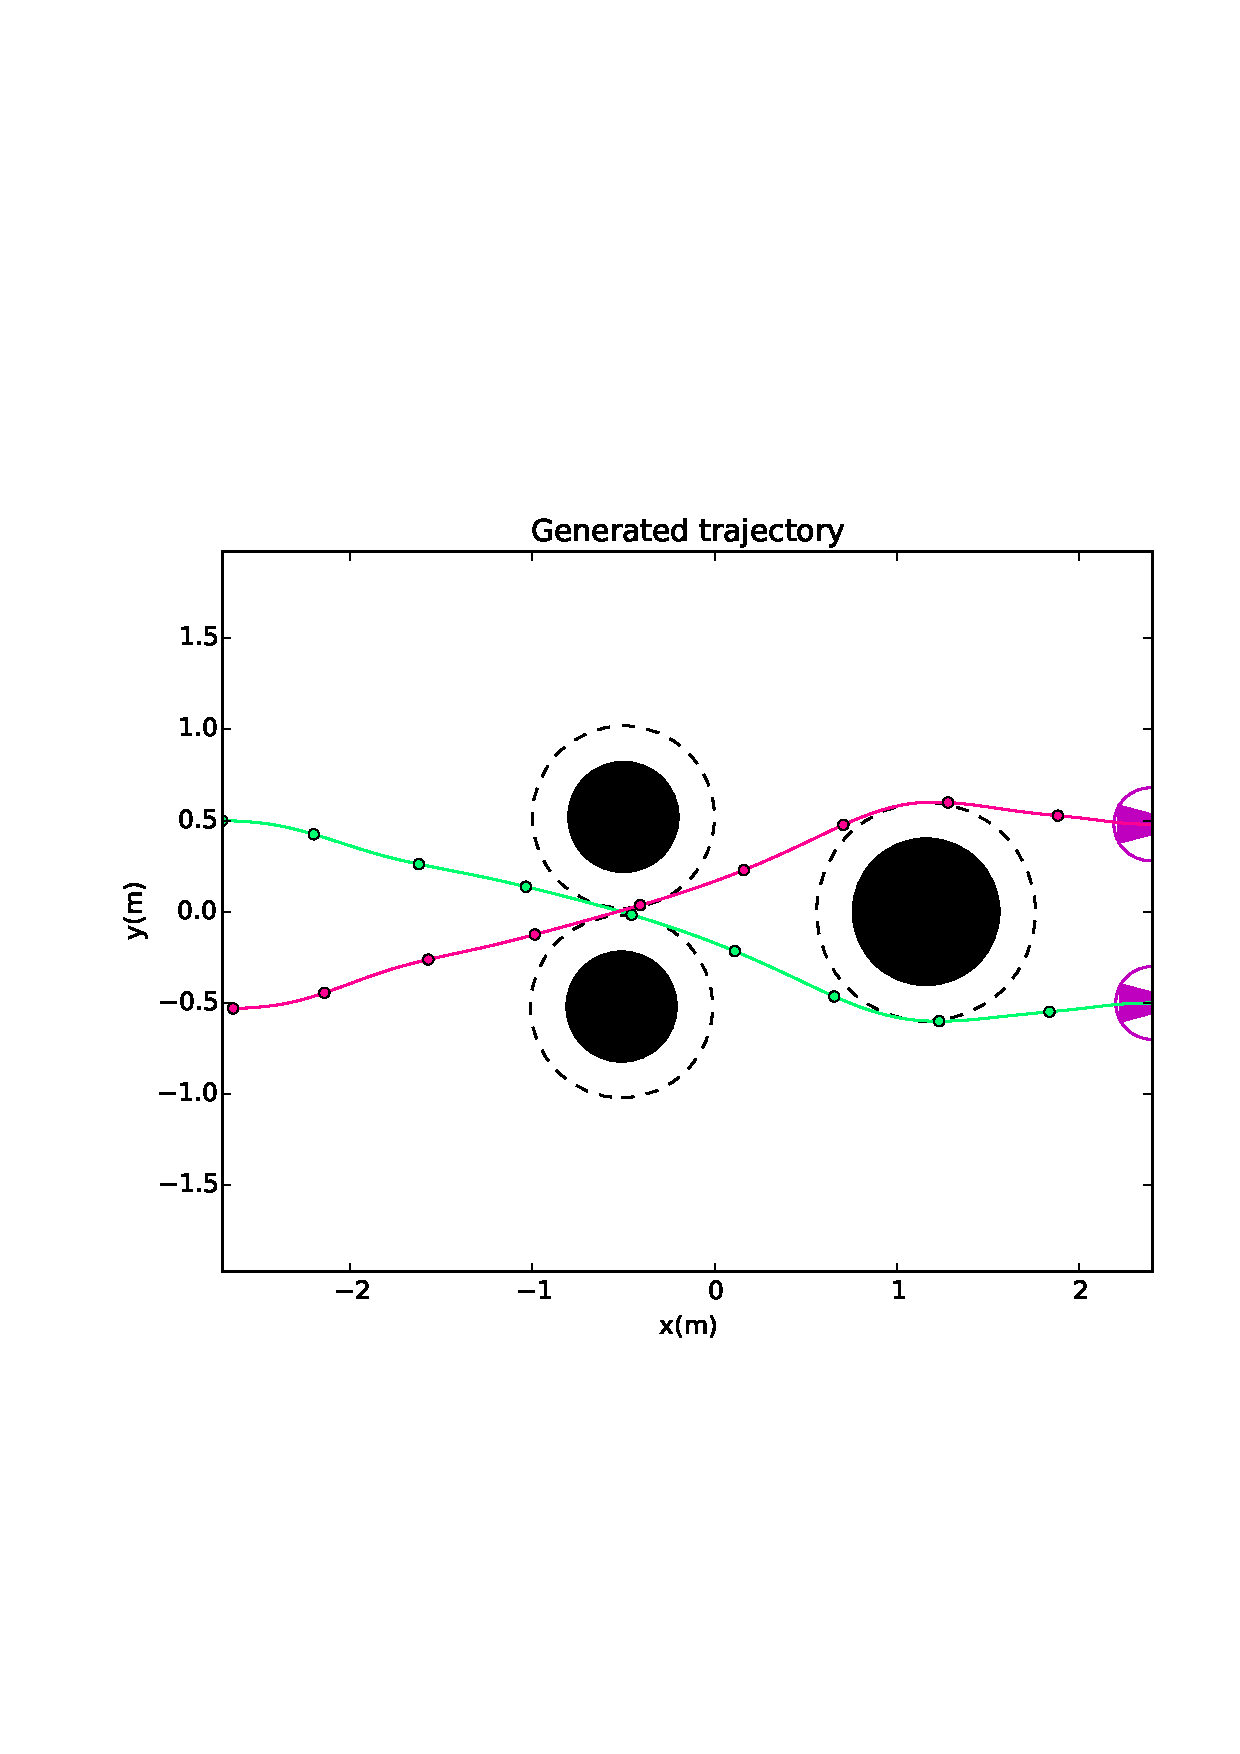
\includegraphics[width=\textwidth]{./images/pwc.png}
                \caption{Generated paths}\label{fig:pwc}
        \end{subfigure}
        ~ %add desired spacing between images, e. g. ~, \quad, \qquad, \hfill etc.
          %(or a blank line to force the subfigure onto a new line)
        \begin{subfigure}[b]{0.48\textwidth}
                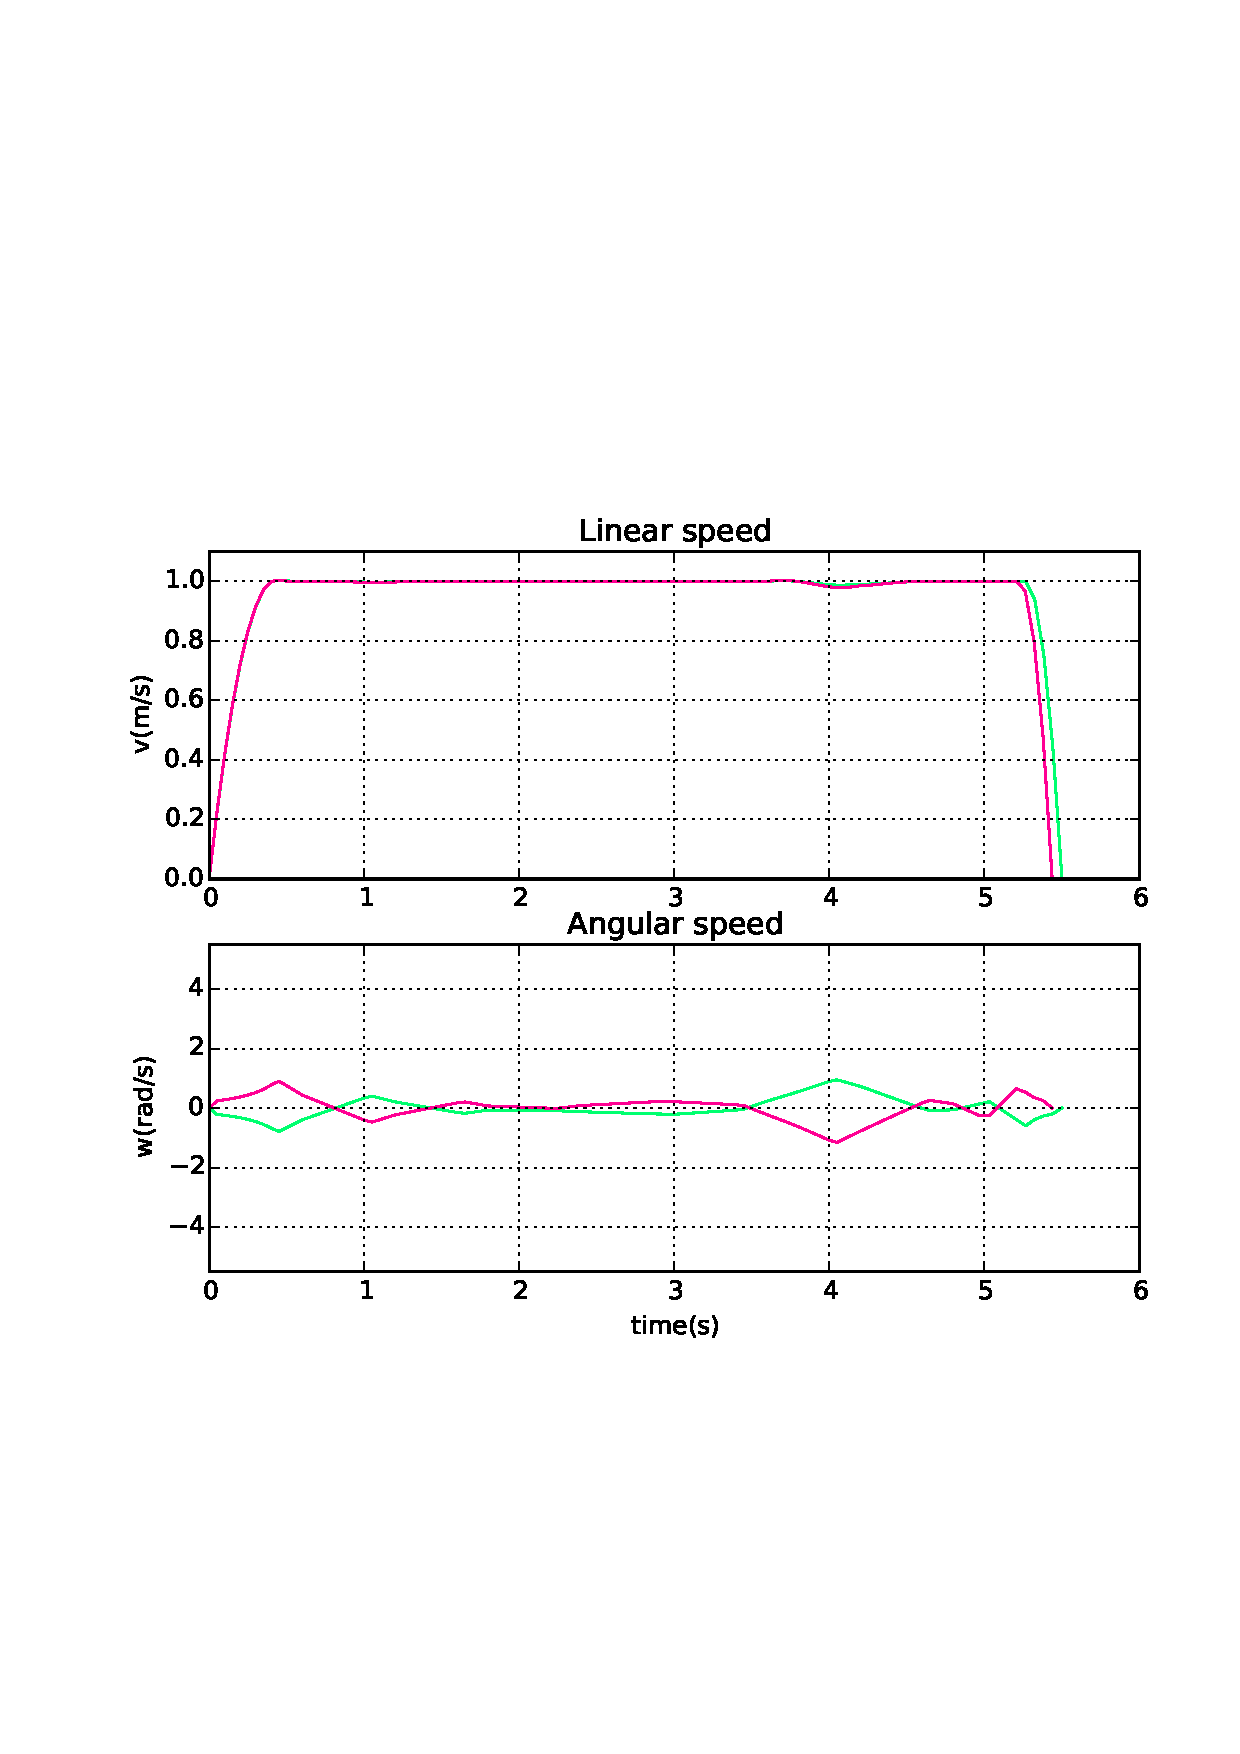
\includegraphics[width=\textwidth]{./images/vwc.png}
                \caption{Velocities}\label{fig:vwc}
        \end{subfigure}
        \caption{multirobot path generation without conflict handling.}\label{fig:wc}
\end{figure}

\begin{figure}[!h]
        \centering
        ~ %add desired spacing between images, e. g. ~, \quad, \qquad, \hfill etc.
          %(or a blank line to force the subfigure onto a new line)
        \begin{subfigure}[b]{0.48\textwidth}
                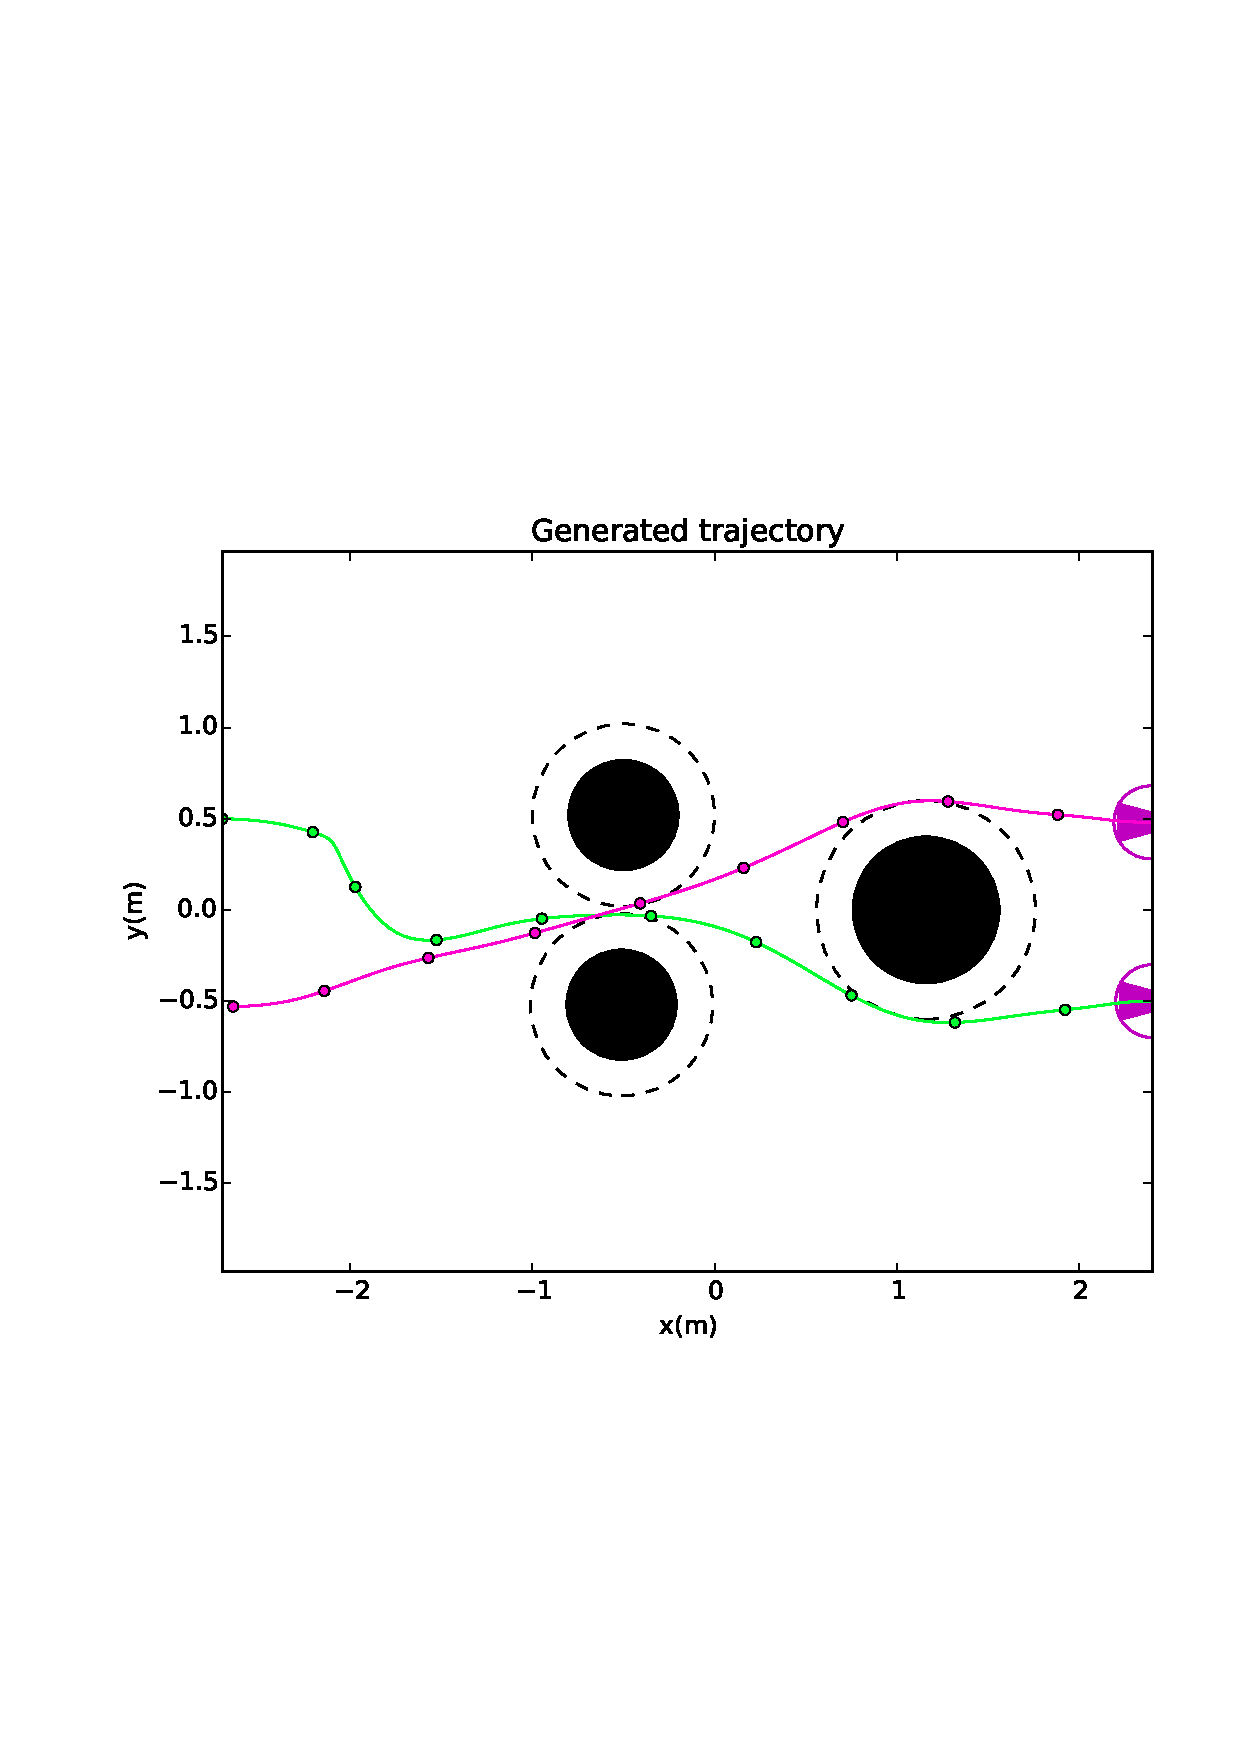
\includegraphics[width=\textwidth]{./images/pnc.png}
                \caption{Generate paths}\label{fig:pnc}
        \end{subfigure}
        ~ %add desired spacing between images, e. g. ~, \quad, \qquad, \hfill etc.
          %(or a blank line to force the subfigure onto a new line)
        \begin{subfigure}[b]{0.48\textwidth}
                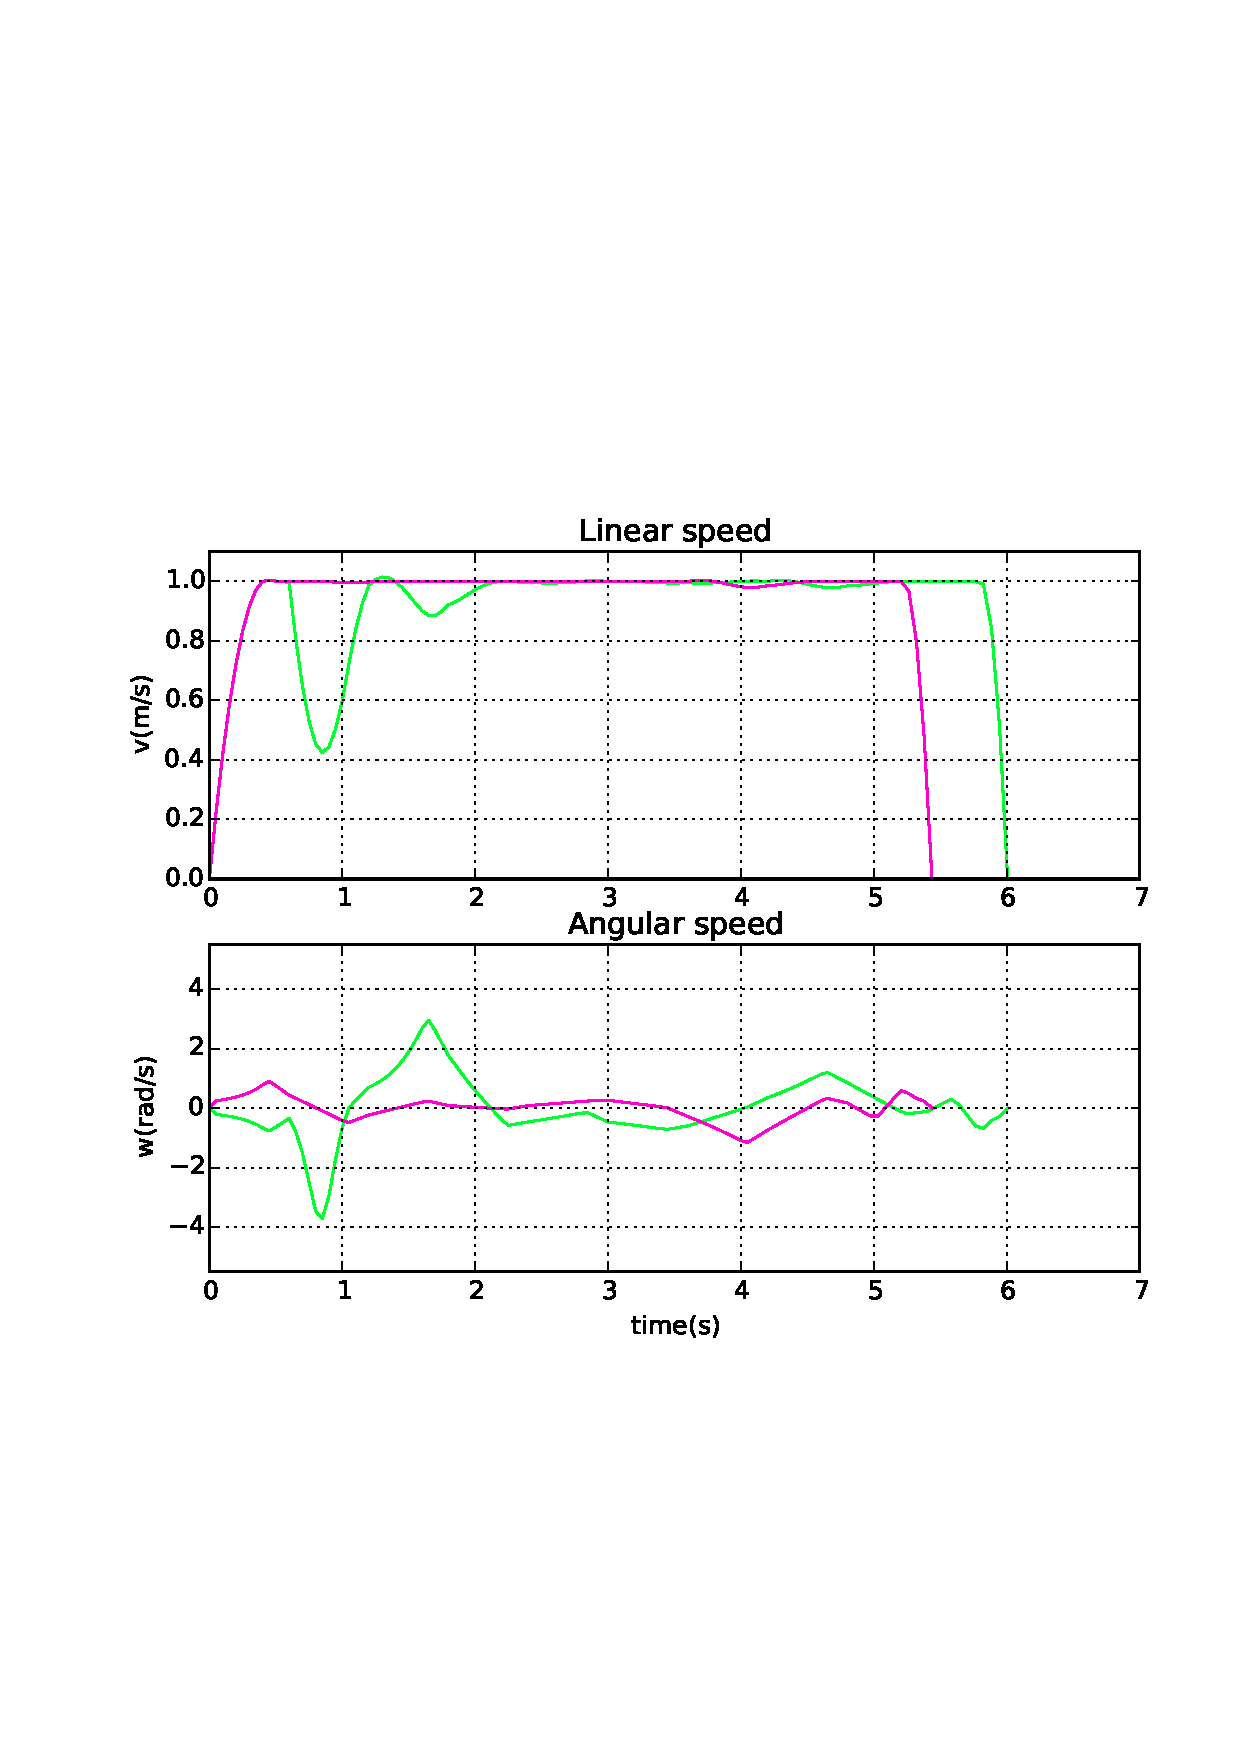
\includegraphics[width=\textwidth]{./images/vnc.png}
                \caption{Velocities}\label{fig:vnc}
        \end{subfigure}
        \caption{multirobot path generation with conflict handling.}\label{fig:nc}
\end{figure}

%\clearpage
\subsection{Analyzing the parameters impact on real-time feasibility and solution fitness}

The performance of the motion planning algorithm previously presented depends on several parameters. For starters these parameters can be split into two groups. The \textbf{algorithm related} parameters and the \textbf{optimization solver related} ones. Among the former group the most important ones are: the number of sample for time discretization ($N_s$), the number of internal knots for the B-splines curves ($n_{knots}$), and the planning and computation time horizons for the sliding windows ($T_p$ and $T_c$ respectively). The latter kind depends on the optimization solver adopted but since most of them are iterative methods is common to have at least a "maximum number of iterations" and a "stop condition" parameters.

The task of searching for a satisfactory set of parameters' values with regard to a performance metric (e.g. total time to complete the mission) is quite laborious.

We attempted nevertheless to extract some quantitative knowledge about how these parameters impact the generated solution based on several simulations run with different parameters configurations. The main objective here is to be able to support the feasibility of a real-time motion planner based on this algorithm.

Omitting some details about the simulations conditions we present one of the many data used in our analyze in the figures. 

We can notice a impact of the number of samples ($N_s$) and number of non-null internal knots ($N_{knots}$). The greater the $N_{knots}$ or the $N_s$ the greater is the \textit{maximum computational time}/$T_c$\footnote{in order to quarantine real-time this ratio has to be inferior to one}. This behavior is the one expected since the number of constraints and the number of arguments for the cost function to be minimized depend on these two parameters respectively.

We were also able to characterize the influence of the number of obstacles seen at once in the computation time and path quality.

Finally we proposed some metric to characterize the fitness of a found solution based on the total time spend going from the initial to the final pose and on the proximity to the obstacles.

%INFO:R0: TOT: 7.57429378065
%INFO:R0: NSE: 15
%INFO:R0: FIR: 1.07032418251
%INFO:R0: LAS: 0.402824163437
%INFO:R0: LMA: 1
%INFO:R0: MAX: 0.243094921112
%INFO:R0: MIN: 0.0298509597778
%INFO:R0: AVG: 0.156346522845
%INFO:R0: RMP: 0.506447752317
%INFO:R0: RMG: 0.83921700716
%p_3_0.48_2.4_11_4_0.001_15_40_20_5.0_0.1_3.0_0.5_1.0_10.0

\begin{figure}[!h]
        \centering
        ~ %add desired spacing between images, e. g. ~, \quad, \qquad, \hfill etc.
          %(or a blank line to force the subfigure onto a new line)
        \begin{subfigure}[b]{0.48\textwidth}
                \includegraphics[width=\textwidth]{./images/realtime/Scenario_3__N_knots_4/mcttc-tctp.eps}
                \caption{Four internal knots. Average variance between lines is $1.047\times 10^{-2}$}\label{fig:uni34}
        \end{subfigure}
        
        ~ %add desired spacing between images, e. g. ~, \quad, \qquad, \hfill etc.
          %(or a blank line to force the subfigure onto a new line)
        \begin{subfigure}[b]{0.48\textwidth}
                \includegraphics[width=\textwidth]{./images/realtime/Scenario_3__N_knots_5/mcttc-tctp.eps}
                \caption{Five internal knots. Average variance between lines is $0.972\times 10^{-2}$}\label{fig:uni35}
        \end{subfigure}
        ~ %add desired spacing between images, e. g. ~, \quad, \qquad, \hfill etc.
          %(or a blank line to force the subfigure onto a new line)
        \begin{subfigure}[b]{0.48\textwidth}
                \includegraphics[width=\textwidth]{./images/realtime/Scenario_3__N_knots_6/mcttc-tctp.eps}
                \caption{Six internal knots. Average variance between lines is $0.587\times 10^{-2}$}\label{fig:uni36}
        \end{subfigure}
        \caption{Three obstacles scenario.}\label{fig:uni3}
\end{figure}

%\begin{table}[!h]
%\caption {Motion planner main parameters} \label{tab:s3param}
%\begin{center}
%\begin{tabular}{|c|c|}
%\hline
%$T_p$ & 2.40 s\\
%\hline 
%$T_c$ & 0.48 s\\
%\hline 
%$N_s$ & 11\\
%\hline 
%$N_{knots}$ & 4\\
%\hline
%$v_{max}$ & $1.00\ \mathrm{m/s}$\\
%\hline
%$\omega_{max}$ & $5.00\ \mathrm{rad/s}$\\
%\hline
%$q_{inital}$ & $[-0.05\ 0.00\ \pi/2]^T$\\
%\hline
%$q_{final}$ & $[0.10\ 7.00\ \pi/2]^T$\\
%\hline
%$u_{final}$ & $[0.00\ 0.00]^T$\\
%\hline
%$u_{final}$ & $[0.00\ 0.00]^T$\\
%\hline
%$O_0$ & $[0.55\ 1.91\ 0.31]$\\
%\hline
%$O_1$ & $[-0.08\ 3.65\ 0.32]$\\
%\hline
%$O_2$ & $[0.38\ 4.65\ 0.16]$\\
%\hline
%\end{tabular}
%\end{center}
%\end{table}

\begin{figure}[!h]
        \centering
        ~ %add desired spacing between images, e. g. ~, \quad, \qquad, \hfill etc.
          %(or a blank line to force the subfigure onto a new line)
        \begin{subfigure}[b]{0.48\textwidth}
                \includegraphics[width=\textwidth]{./images/realtime/sim_results/p_3_0.48_2.4_11_4_0.001_15_40_20_5.0_0.1_3.0_0.5_1.0_10.0/multirobot-path.png}
                \caption{Robot's path.}\label{fig:rpath}
        \end{subfigure}
        ~ %add desired spacing between images, e. g. ~, \quad, \qquad, \hfill etc.
          %(or a blank line to force the subfigure onto a new line)
        \begin{subfigure}[b]{0.48\textwidth}
		\includegraphics[width=\textwidth]{./images/realtime/sim_results/p_3_0.48_2.4_11_4_0.001_15_40_20_5.0_0.1_3.0_0.5_1.0_10.0/multirobot-vw.png}
                \caption{Robot's input.}\label{fig:rinput}
        \end{subfigure}
        \caption{Three obstacle scenario simulation example where the \textit{maximum computational time} was about 84\% of $T_c$ and the mission total time equals to $7.57\ s$.}\label{fig:uni3}
\end{figure}

%\clearpage
\subsection{From Python to C++ using the XDE simulator}

XDE is a physics simulation software environment fully developed by CEA-LIST that can handle a variety of physical aspects such as deformable bodies, multibody systems with kinematic constraints and contacts, and fluids.

Its utilization presents though some rough edges and a steep learning curve.

During the third month and beginning of the forth while producing the analysis referenced by the latest subsection we begin porting the implementation done in python to the XDE environment. 

The objective is to get much closer to a real physical system being able to implement in the simulated environment notions neglected at the first months. For instance the obstacle detection can be based on real sensors models carrying uncertainties instead of assuming the absolute knowledge of an obstacle position as soon as it enters within the robot's detection radius.

% \todo[inline, color=green!40]{develop this article}
% \cite{Gao2006}
%\clearpage
\section{Conclusion}
% \todo[inline, color=green!40]{Quels sont les avantages et inconvénients des techniques étudiées ? Quelles sont les limites de ces méthodes ? Quelles sont les hypothèses "cachées" que font ces méthodes ? ...}

The work done until now is promising. We implemented and did some minors improvements on the solution proposed by \cite{Defoort2007a}, we gather a good understanding of the impact of the algorithm's parameters in the computation cost and in the quality of the solution and we started the porting of the algorithm to a more realistic simulation environment.
%\clearpage
\section{Perspectives}
% \todo[inline, color=green!40]{Est-ce que le problème est résolu ? Quels axes d'amélioration peut-on envisager ?}

We hope being able to write a paper focused on the impact of the algorithm's parameters on the computation cost and on the solution quality  for submitting to the International Workshop on On-line Decision-Making in Multi-Robot Coordination.

During the months to came we also hope to develop the current approach so it can address dynamic obstacles.

% Commands to include a figure:
% \begin{figure}
% \centering
% \includegraphics[width=0.5\textwidth]{frog.jpg}
% \caption{\label{fig:frog}This is a figure caption.}
% \end{figure}


% \bibliographystyle{unsrt}
%\clearpage
\selectlanguage{english}
%\nocite{*}
\bibliography{references}
\bibliographystyle{plain}


\end{document}